%%%%%% Run at command line, run
%%%%%% xelatex grad-sample.tex 
%%%%%% for a few times to generate the output pdf file
\documentclass[12pt,oneside,openright,a4paper]{cpe-thai-project}


\usepackage{polyglossia}
\usepackage{enumitem,lipsum}
\usepackage{graphicx}
\usepackage{placeins}
\usepackage{tabularx}
\usepackage{multirow}
\usepackage{colortbl}
\usepackage{graphicx}
\usepackage[table,xcdraw]{xcolor}

\graphicspath{ {./images/} }
\setdefaultlanguage{thai}
\setotherlanguage{english}
\newfontfamily\thaifont[Script=Thai,Scale=1.23]{TH Sarabun New}
\defaultfontfeatures{Mapping=tex-text,Scale=1.23,LetterSpace=0.0}
\setmainfont[Scale=1.23,LetterSpace=0,WordSpace=1.0,FakeStretch=1.0,Mapping=tex-text]{TH Sarabun New}
\XeTeXlinebreaklocale "th"	
\XeTeXlinebreakskip = 0pt plus 0pt
\emergencystretch=10pt

%%%%%%%%%%%%%%%%%%%%%%%%%%%%%%%%%%%%%%%%%%%%%%%%%%%%%%%%%%%%%%%%%%%
% Customize below to suit your needs 
% The ones that are optional can be left blank. 
%%%%%%%%%%%%%%%%%%%%%%%%%%%%%%%%%%%%%%%%%%%%%%%%%%%%%%%%%%%%%%%%%%%
% First line of title
\def\disstitleone{Will Chain }   
% Second line of title
\def\disstitletwo{Will On Blockchain}   
% Your first name and lastname
\def\dissauthor{MR. THITIPONG BOONTHANAKORN}   % 1st member
%%% Put other group member names here ..
\def\dissauthortwo{MR. NARONGYOT SOONTHARARAK}   % 2nd member (optional)
\def\dissauthorthree{MR. SUBTAWEE NGANRUNGRUANG}   % 3rd member (optional)


% The degree that you're persuing..
\def\dissdegree{Bachelor of Engineering} % Name of the degree
\def\dissdegreeabrev{B.Eng} % Abbreviation of the degree
\def\dissyear{2022}                   % Year of submission
\def\thaidissyear{2565}               % Year of submission (B.E.)

%%%%%%%%%%%%%%%%%%%%%%%%%%%%%%%%%%%%%%%%%%%%
% Your project and independent study committee..
%%%%%%%%%%%%%%%%%%%%%%%%%%%%%%%%%%%%%%%%%%%%
\def\dissadvisor{Asst.Prof. Marong Phadoongsidhi, Ph.D.}  % Advisor
%%% Leave it empty if you have no Co-advisor
\def\disscoadvisor{}  % Co-advisor
\def\disscommitteetwo{Dr. Piyanit Wepulanon , Ph.D.}  % 3rd committee member (optional)
\def\disscommitteethree{Assoc.Prof. Thumrongrat Amornraksa , Ph.D.}
\def\disscommitteefour{Asst.Prof. Surapont Toomnark}    % 5th committee member (optional) 

\def\worktype{Project} %%  Project or Independent study
\def\disscredit{3}   %% 3 credits or 6 credits


\def\fieldofstudy{Computer Engineering} 
\def\department{Computer Engineering} 
\def\faculty{Engineering}

\def\thaifieldofstudy{วิศวกรรมคอมพิวเตอร์} 
\def\thaidepartment{วิศวกรรมคอมพิวเตอร์} 
\def\thaifaculty{วิศวกรรมศาสตร์}
 
\def\appendixnames{Appendix} %%% Appendices or Appendix

\def\thaiworktype{ปริญญานิพนธ์} %  Project or research project % 
\def\thaidisstitleone{Will Chain}
\def\thaidisstitletwo{Will on Blockchain}
\def\thaidissauthor{นายฐิติพงศ์ บุณธนากร}
\def\thaidissauthortwo{นายณรงค์ยศ สุนทรารักษ์} %Optional
\def\thaidissauthorthree{นายทรัพย์ทวี งานรุ่งเรือง} %Optional

\def\thaidissadvisor{ผศ.ดร.มารอง ผดุงสิทธิ์}
%% Leave this empty if you have no co-advisor
\def\thaidisscoadvisor{รศ.ดร.ที่ปรึกษา วิทยานิพนธ์ร่วม} %Optional
\def\thaidissdegree{วิศวกรรมศาสตรบัณฑิต}

% Change the line spacing here...
\linespread{1.15}

%%%%%%%%%%%%%%%%%%%%%%%%%%%%%%%%%%%%%%%%%%%%%%%%%%%%%%%%%%%%%%%%
% End of personal customization.  Do not modify from this part 
% to \begin{document} unless you know what you are doing...
%%%%%%%%%%%%%%%%%%%%%%%%%%%%%%%%%%%%%%%%%%%%%%%%%%%%%%%%%%%%%%%%


%%%%%%%%%%%% Dissertation style %%%%%%%%%%%
%\linespread{1.6} % Double-spaced  
%%\oddsidemargin    0.5in
%%\evensidemargin   0.5in
%%%%%%%%%%%%%%%%%%%%%%%%%%%%%%%%%%%%%%%%%%%
%\renewcommand{\subfigtopskip}{10pt}
%\renewcommand{\subfigbottomskip}{-5pt} 
%\renewcommand{\subfigcapskip}{-6pt} %vertical space between caption
%                                    %and figure.
%\renewcommand{\subfigcapmargin}{0pt}

\renewcommand{\topfraction}{0.85}
\renewcommand{\textfraction}{0.1}

\newtheorem{theorem}{Theorem}
\newtheorem{lemma}{Lemma}
\newtheorem{corollary}{Corollary}

\def\QED{\mbox{\rule[0pt]{1.5ex}{1.5ex}}}
\def\proof{\noindent\hspace{2em}{\itshape Proof: }}
\def\endproof{\hspace*{\fill}~\QED\par\endtrivlist\unskip}
%\newenvironment{proof}{{\sc Proof:}}{~\hfill \blacksquare}
%% The hyperref package redefines the \appendix. This one 
%% is from the dissertation.cls
%\def\appendix#1{\iffirstappendix \appendixcover \firstappendixfalse \fi \chapter{#1}}
%\renewcommand{\arraystretch}{0.8}
%%%%%%%%%%%%%%%%%%%%%%%%%%%%%%%%%%%%%%%%%%%%%%%%%%%%%%%%%%%%%%%%
%%%%%%%%%%%%%%%%%%%%%%%%%%%%%%%%%%%%%%%%%%%%%%%%%%%%%%%%%%%%%%%%

\usepackage{ragged2e}
\begin{document}

\pdfstringdefDisableCommands{%
\let\MakeUppercase\relax
}

\begin{center}
  
\includegraphics[width=2.8cm]{logo02.jpg}
\end{center}
\vspace*{-1cm}

\maketitlepage
\makesignaturepage 

%%%%%%%%%%%%%%%%%%%%%%%%%%%%%%%%%%%%%%%%%%%%%%%%%%%%%%%%%%%%%%
%%%%%%%%%%%%%%%%%%%%%% English abstract %%%%%%%%%%%%%%%%%%%%%%%
%%%%%%%%%%%%%%%%%%%%%%%%%%%%%%%%%%%%%%%%%%%%%%%%%%%%%%%%%%%%%%
\abstract


Will Chain is a developed platform aimed at studying the workings of the Blockchain network and managing the inheritance of both real-world assets and digital assets. It incorporates features that facilitate the preservation of existing wills to meet the requirements of asset transactions in both the physical and digital realms, specifically in the form of Non-Fungible Tokens (NFTs). Additionally, it includes features for securely delivering assets to the intended recipients, provided that the conditions specified in the will are met. This enhances security, trustworthiness, and convenience in the process of asset succession through wills. Overall, Will Chain offers a more comprehensive and improved framework for executing asset transactions compared to traditional methods.

\begin{flushleft}
\begin{tabular*}{\textwidth}{@{}lp{0.8\textwidth}}
 & \\
\textbf{Keywords}: & Asset / Blockchain / Cryptocurrency / Digital Asset / Non-Fungible Token (NFT) / Real Asset /  Smart Contract / Will 
\end{tabular*}
\end{flushleft}
\endabstract

%%%%%%%%%%%%%%%%%%%%%%%%%%%%%%%%%%%%%%%%%%%%%%%%%%%%%%%%%%%%%%
%%%%%%%%%% Thai abstract here %%%%%%%%%%%%%%%%%%%%%%%%%%%%%%%%%
%%%%%%%%%%%%%%%%%%%%%%%%%%%%%%%%%%%%%%%%%%%%%%%%%%%%%%%%%%%%%%
% {\newfontfamily\thaifont{TH Sarabun New:script=thai}[Scale=1.3]
% \XeTeXlinebreaklocale "th_TH"	
% \thaifont
\newcommand\tab[1][1cm]{\hspace*{#1}}
\thaiabstract

Will Chain เป็นแพลตฟอร์มที่พัฒนาขึ้นเพื่อศึกษาการทำงานของเครือข่าย Blockchain และจัดการพินัยกรรมสินทรัพย์ทั้งในโลกความเป็นจริงและสินทรัพย์ดิจิทัล โดย Will Chain มีฟีเจอร์ในการเก็บรักษาพินัยกรรมที่มีอยู่ในปัจจุบัน เพื่อสอดคล้องต่อความต้องการในการทำพินัยกรรมทั้งในสินทรัพย์จริงและสินทรัพย์ดิจิทัลในรูปแบบของ Non-Fungible Token (NFT) นอกจากนี้ยังมีฟีเจอร์สำหรับการส่งมอบสินทรัพย์ให้กับผู้รับพินัยกรรม ในกรณีที่เงื่อนไขตรงกับในพินัยกรรม ซึ่งช่วยเพิ่มความปลอดภัย ความน่าเชื่อถือ และความสะดวกในกระบวนการสืบทอดสินทรัพย์ผ่านพินัยกรรม โดยรวม Will Chain มีความครอบคลุมและสนับสนุนการทำพินัยกรรมอย่างเป็นอย่างดีกว่าเดิม
\begin{flushleft}
\begin{tabular*}{\textwidth}{@{}lp{0.8\textwidth}}
 & \\

\textbf{คำสำคัญ}: & Asset / Blockchain / Cryptocurrency / Digital Asset / Non-Fungible Token (NFT) / Real Asset /  Smart Contract / Will 
\end{tabular*}
\end{flushleft}
\endabstract

%}

%%%%%%%%%%%%%%%%%%%%%%%%%%%%%%%%%%%%%%%%%%%%%%%%%%%%%%%%%%%%
%%%%%%%%%%%%%%%%%%%%%%% Acknowledgments %%%%%%%%%%%%%%%%%%%%
%%%%%%%%%%%%%%%%%%%%%%%%%%%%%%%%%%%%%%%%%%%%%%%%%%%%%%%%%%%%
\preface
\tab การพัฒนาโครงงาน Will Chain ในครั้งนี้สําเร็จลงได้ด้วยความช่วยเหลือของ ผู้ช่วยศาสตราจารย์ ดร. มารอง ผดุงสิทธิ์ ที่ปรึกษาโครงงาน ซึ่งได้ให้ความกรุณา สละเวลาให้คําปรึกษา คําแนะนํา ข้อเสนอแนะอันมีประโยชน์อย่างยิ่ง และความช่วยเหลือตลอดการทําโครงงานนี้จนสําเร็จลุล่วงได้ด้วยดี ผู้จัดทําโครงงานจึงขอกราบขอบพระคุณเป็นอย่างสูง

\tab ขอขอบพระคุณ คุณวราณัฐ สุทธิการณ์ ซึ่งได้ให้ความกรุณาสละเวลาให้คําแนะนําการออกแบบ Smart Contract และความช่วยเหลือตลอดการทำโครงงานนี้

\tab ขอขอบพระคุณ ผ.ศ.สุรพนธ์ ตุ้มนาค , ดร.ปิยนิตย์ เวปุลานนท์ และ รศ.ดร.ธํารงรัตน์ อมรรักษา ที่ได้สละเวลา
ร่วมเป็นคณะกรรมการตรวจสอบโครงงานในครั้งนี้ 

\tab ท้ายที่สุดนี้ โครงงานนี้อาจจะไม่สําเร็จเลยหากไม่มีเพื่อนในภาควิชาวิศวกรรมคอมพิวเตอร์ มหาวิทยาลัยเทคโนโลยีพระจอมเกล้าธนบุรีที่ให้ 
ความช่วยเหลือ การสนับสนุน รวมทั้งคอยเป็นกําลังใจสําคัญเสมอมา 

\tab ทีมผู้จัดทำหวังว่าโครงงาน Will Chain นี้จะก่อให้เกิดประโยชน์ต่อการทำพินัยกรรมในปัจจุบัน และสามารถครอบคลุมไปถึงพินัยกรรมของสินทรัพย์ดิจิทัลที่ยังไม่มีเทคโนโลยีรองรับในขณะนี้ และเกิดการเปลี่ยนแปลงที่ดีขึ้นในอนาคต

%%%%%%%%%%%%%%%%%%%%%%%%%%%%%%%%%%%%%%%%%%%%%%%%%%%%%%%%%%%%%
%%%%%%%%%%%%%%%% ToC, List of figures/tables %%%%%%%%%%%%%%%%
%%%%%%%%%%%%%%%%%%%%%%%%%%%%%%%%%%%%%%%%%%%%%%%%%%%%%%%%%%%%%
% The three commands below automatically generate the table 
% of content, list of tables and list of figures
\tableofcontents                    
\listoftables
\listoffigures                      

%%%%%%%%%%%%%%%%%%%%%%%%%%%%%%%%%%%%%%%%%%%%%%%%%%%%%%%%%%%%%%
%%%%%%%%%%%%%%%%%%%%% List of symbols page %%%%%%%%%%%%%%%%%%%
%%%%%%%%%%%%%%%%%%%%%%%%%%%%%%%%%%%%%%%%%%%%%%%%%%%%%%%%%%%%%%
% You have to add this manually..
%\listofsymbols
%
%%%%%%%%%%%%%%%%%%%%%%%%%%%%%%%%%%%%%%%%%%%%%%%%%%%%%%%%%%%%%%
%%%%%%%%%%%%%%%%%%%%% List of vocabs & terms %%%%%%%%%%%%%%%%%
%%%%%%%%%%%%%%%%%%%%%%%%%%%%%%%%%%%%%%%%%%%%%%%%%%%%%%%%%%%%%%
% You also have to add this manually..
\listofvocab
\begin{flushleft}
\begin{tabular}{@{}p{1in}@{=\extracolsep{0.5in}}l}
Asset & ทรัพย์สินที่เรามีอยู่ทั้งหมด  เงินที่อยู่ในบัญชีทั้หรืออยู่ในกระเป๋าทั้งหมด รวมทั้งหนี้สินที่เรามีอยู่ทั้งหมด \\
Blockchain & ระบบโครงข่ายในการเก็บบัญชีธุรกรรมออนไลน์ \\
Cryptocurrency & สกุลเงินเข้ารหัส เป็นสินทรัพย์ดิจิทัล \\
Crypto Wallet & เป็นเครื่องมือที่มีหน้าที่จัดเก็บคีย์ส่วนตัวเพื่อให้เกิดความปลอดภัย อีกทั้งช่วยในการรับ-โอนเงินดิจิทัล\\
Digital Asset & สิ่งที่มีมูลค่าและเราสามารถเป็นเจ้าของได้ แต่ไม่สามารถแตะต้องได้ทางกายภาพ\\
Mint NFT & กระบวนการเปลี่ยนไฟล์งานดิจิทัลให้กลายเป็นชุดการเข้ารหัส หรือสินทรัพย์ดิจิทัลที่จัดเก็บไว้บน Blockchain \\
Non-Fungible Token(NFT) & สิ่งของที่มีความแตกต่างเฉพาะตัวไม่สามารถทดแทนกันได้หรือซื้อเป็นหน่วยย่อยได้\\
Real Asset & สินทรัพย์จริง หรือสินทรัพย์ทีมีอยู่ในโลกความเป็นจริง เช่น ทะเบียนบ้าน \\
Smart Contract & กระบวนการทางดิจิทัล ที่กำหนดขั้นตอนการทำธุรกรรมโดยอัตโนมัติไว้ล่วงหน้า โดยไม่ต้องอาศัยตัวกลาง\\
Web3.0 & การพัฒนาเว็บและแพลตฟอร์มที่ใช้เทคโนโลยี Blockchain เพื่อควบคุมข้อมูลโดยไม่ต้องพึ่งพาบุคคลกลาง\\
Will  & พินัยกรรมที่เก็บคำสั่งเสียสุดท้ายในการทำกิจการต่าง ๆ \\

\end{tabular}
\end{flushleft}

%\setlength{\parskip}{1.2mm}

%%%%%%%%%%%%%%%%%%%%%%%%%%%%%%%%%%%%%%%%%%%%%%%%%%%%%%%%%%%%%%%
%%%%%%%%%%%%%%%%%%%%%%%% Main body %%%%%%%%%%%%%%%%%%%%%%%%%%%%
%%%%%%%%%%%%%%%%%%%%%%%%%%%%%%%%%%%%%%%%%%%%%%%%%%%%%%%%%%%%%%%


\chapter{บทนำ}

\section{ที่มาและความสำคัญ}

\tab ในปัจจุบันเทคโนโลยีมีบทบาทสำคัญในชีวิตของผู้คนในหลายด้าน เช่นการเงินและสินทรัพย์ อย่างไรก็ตาม พินัยกรรมเป็นเอกสารที่ยังไม่ได้รับประโยชน์จากเทคโนโลยีในปัจจุบัน ซึ่งมักจะต้องเก็บรักษาเอกสารดังกล่าวเองหรือใช้ทนายควบคุม นั่นอาจทำให้เกิดความเสียหายหรือสูญหายได้ และอาจมีโอกาสที่ข้อมูลจะถูกเปลี่ยนแปลงจากบุคคลที่สาม ทำให้กระบวนการทำพินัยกรรมมีความไม่ปลอดภัย นอกจากนี้ พินัยกรรมในปัจจุบันยังไม่รองรับเกี่ยวกับการสืบทอดสินทรัพย์ดิจิทัล เช่น Cryptocurrency เนื่องจากยังไม่มีเทคโนโลยี และกฏหมายที่รองรับในปัจจุบัน

\tab จึงเกิดแนวคิดในการสร้างแพลตฟอร์มสำหรับจัดการพินัยกรรมทั้งในโลกความเป็นจริงและสินทรัพย์ดิจิทัลผ่านระบบ Blockchain โดยสามารถนำพินัยกรรมที่มีอยู่ในปัจจุบันมาบันทึกใน Blockchain เพื่อเก็บรักษา เพิ่มความน่าเชื่อถือ และทำการสืบทอดสินทรัพย์ไปยังผู้รับพินัยกรรม รวมทั้งรองรับสินทรัพย์ดิจิทัลอีกด้วย การคำนึงถึงความปลอดภัยและความสะดวกสบายของผู้ใช้งานเป็นสิ่งสำคัญในแพลตฟอร์มนี้


\section{วัตถุประสงค์}

\begin{itemize}
\item เพื่อศึกษาเทคโนโลยี Blockchain
\item เพื่อสร้างแพลตฟอร์มสำหรับจัดการพินัยกรรมทั้งสินทรัพย์ในโลกความเป็นจริง และสินทรัพย์ดิจิทัล
\item เพื่อให้พินัยกรรมในปัจจุบันสามารถครอบคลุมถึงสินทรัพย์ดิจิทัล
\item เพื่อเก็บรักษาพินัยกรรมให้มีความปลอดภัยมากขึ้น และมีความน่าเชื่อถือ
\item เพื่ออำนวยความสะดวกในการจัดเก็บพินัยกรรม
\end{itemize}

\section{ขอบเขตของโครงงาน}

\begin{itemize}
\item พัฒนาแพลตฟอร์มพินัยกรรมที่สามารถใช้งานได้บน Ethereum chain (Test-network) เท่านั้น
\item ใช้ภาษา Solidity ในการพัฒนา Smart Contract
\item รองรับ Crypto Wallet ได้แก่ MetaMask Wallet เพียงเท่านั้น
\item พัฒนาแพลตฟอร์มสำหรับจัดการพินัยกรรมทั้งสินทรัพย์ในโลกความเป็นจริง และสินทรัพย์ดิจิทัล
\end{itemize}

\section{ประโยชน์ที่คาดว่าจะได้่รับ}
\tab Will Chain เป็นการใช้เทคโนโลยี Blockchain เพื่อประยุกต์ต่อการจัดเก็บพินัยกรรม และสืบทอดสินทรัพย์ทั้งสินทรัพย์จริงและสินทรัพย์ดิจิทัลจากผู้ทำพินัยกรรมไปหาผู้รับสินทรัพย์ได้ด้วยรูปแบบของ Non-Fungible Token(NFT)
\section{เนื้อหาทางวิศวกรรมที่เป็นต้นฉบับ}
\tab โครงการนี้ได้ถูกพัฒนาขึ้นโดยใช้ความรู้ในการทำงานของเทคโนโลยีบล็อกเชน (Blockchain Technology) โดยใช้เครื่องมือในการพัฒนาสมาร์ทคอนแทรกต์ (Smart Contract) ด้วยภาษา Solidity เป็นส่วนหนึ่งของโครงการ นอกจากนี้ยังใช้ความรู้ในเรื่องของ Non-Fungible Token (NFT) เพื่อใช้ในการเก็บข้อมูลพินัยกรรมที่เกี่ยวข้องกับโครงการนี้ รวมถึงการทำ Decentralized Web Application โดยใช้ Next.js (Typescript Framework) เป็นเครื่องมือในการพัฒนาส่วนติดต่อกับผู้ใช้ และได้ใช้ความรู้ด้านวิศวกรรมซอฟต์แวร์และพินัยกรรมเพื่อให้สามารถทำการถ่ายทอดพินัยกรรมได้ภายใน Decentralized Web Application นี้
\clearpage

\section{การแยกย่อยงาน และร่างแผนคำแนะนำจากอาจารย์ที่ปรึกษา}
\begin{enumerate}
\item ศึกษาค้นคว้าที่มาและความสำคัญของปัญหา
\item เสนอหัวข้อโครงการให้กับอาจารย์ที่ปรึกษา
\item ทำการสำรวจหรือศึกษาค้นคว้าข้อมูลที่เกี่ยวข้องกับโครงงาน
	\begin{itemize}
		\item ศึกษาเรื่องพินัยกรรม
		\item ศึกษาเรื่องกฎหมาย
		\item ศึกษาเรื่องสินทรัพย์
	\end{itemize}
\item นำเสนอโครงการและข้อมูลทึ่ศึกษาค้นคว้าให้กับอาจารย์ที่ปรึกษา
\item จัดทำข้อเสนอโครงการ
\item นำเสนอข้อเสนอโครงการ
\item จัดทำรายงาน
	\begin{itemize}
		\item รายงานบทที่ 1 จากข้อมูลข้อเสนอโครงงาน
		\item รายงานบทที่ 2 จากข้อมูลการศึกษาค้นคว้าเกี่ยวกับทฤษฎีที่เกี่ยวข้อง
		\item รายงานบทที่ 3 รายงานการออกแบบการทำงานของระบบเบื้องต้น
	\end{itemize}
\item วิเคราะห์และออกแบบระบบ
	\begin{itemize}
		\item ออกแบบการทำงาน Algorithms ของ Smart Contract ที่ใช้งานในระบบ
		\item ออกแบบรูปแบบพินัยกรรมที่จะใช้ในระบบ
		\item ออกแบบส่วนของผู้ใช้งาน (UX/UI)
	\end{itemize}
\item ศึกษาและพัฒนา Blockchain และ Smart Contract
	\begin{itemize}
		\item ศึกษาการทำงานของ Blockchain โดยเลือกใช้ Ethereum chain
		\item ศึกษาและพัฒนาส่วนของ Smart Contract ที่ใช้ในการควบคุมระบบด้วยภาษา Solidity
		\item ศึกษาและพัฒนา Non-Fungible Token (NFT) ในระบบ
	\end{itemize}
\item ศึกษาและพัฒนา Web application
	\begin{itemize}
		\item ศึกษาและพัฒนาส่วนของผู้ใช้งานด้วย Next.js Typescript และ User Interface Framework อื่น ๆ 
		\item ศึกษาเกี่ยวกับ API ของหน่วยงานรัฐ
		\item ศึกษาเกี่ยวกับการเชื่อมต่อกับ Smart Contract
	\end{itemize}
\item นำเสนอโครงงาน 3 บท
\item ศึกษาและพัฒนา Blockchain และ Smart Contract (ต่อจากภาคการศึกษาที่ 1)
\item ทดสอบการทำงานของ Ethereum chain
\item ปรับปรุงและแก้ไข Ethereum chain
\item ศึกษาและพัฒนา Web application (ต่อจากภาคการศึกษาที่ 1)
\item ทดสอบการทำงานของ Web application
\item ปรับปรุงและแก้ไข Web application
\item จัดทำรายงงานโครงงานฉบับสมบูรณ์
\item นำเสนอโครงงาน
\end{enumerate}
\clearpage
\section{ตารางการดำเนินงาน}

\begin{table}[h]
	\centering
	\caption{ตารางการดำเนินงาน ประจำภาคการศึกษาที่ 1/2565}
	\resizebox{\linewidth}{!}{%
		\begin{tabular}{|l|l|l|l|l|l|l|l|l|l|l|l|l|l|l|l|l|l|l|l|l|l|} 
		\hline
		\multicolumn{22}{|c|}{ตารางการดำเนินงาน ประจำภาคการศึกษาที่ 1/2565}                                                                                                                                                                                                                                                                                                                                                                                                                                                                                                                                                                                                                                                                                                                                                                                                                                                   \\ 
		\hline
		\multicolumn{1}{|c|}{\multirow{3}{*}{ที่}} & \multicolumn{1}{c|}{\multirow{3}{*}{หัวข้อการดำเนินงาน}}    & \multicolumn{20}{c|}{ระยะเวลา}                                                                                                                                                                                                                                                                                                                                                                                                                                                                                                                                                                                                                                                                                                                                                                             \\ 
		\cline{3-22}
		\multicolumn{1}{|c|}{}                     & \multicolumn{1}{c|}{}                                       & \multicolumn{4}{c|}{สิงหาคม}                                                                                                                              & \multicolumn{4}{c|}{กันยายน}                                                                                                                              & \multicolumn{4}{c|}{ตุลาคม}                                                                                                                               & \multicolumn{4}{c|}{พฤศจิกายน}                                                                                                                            & \multicolumn{4}{c|}{ธันวาคม}                                                                                                                               \\ 
		\cline{3-22}
		\multicolumn{1}{|c|}{}                     & \multicolumn{1}{c|}{}                                       & \multicolumn{1}{c|}{1}               & \multicolumn{1}{c|}{2}               & \multicolumn{1}{c|}{3}               & \multicolumn{1}{c|}{4}               & \multicolumn{1}{c|}{1}               & \multicolumn{1}{c|}{2}               & \multicolumn{1}{c|}{3}               & \multicolumn{1}{c|}{4}               & \multicolumn{1}{c|}{1}               & \multicolumn{1}{c|}{2}               & \multicolumn{1}{c|}{3}               & \multicolumn{1}{c|}{4}               & \multicolumn{1}{c|}{1}               & \multicolumn{1}{c|}{2}               & \multicolumn{1}{c|}{3}               & \multicolumn{1}{c|}{4}               & \multicolumn{1}{c|}{1}               & \multicolumn{1}{c|}{2}               & \multicolumn{1}{c|}{3}               & \multicolumn{1}{c|}{4}                \\ 
		\hline
		1                                          & ศึกษาค้นคว้าที่มาของและ ความสำคัญของปัญหา                   & {\cellcolor[rgb]{0.176,0.549,0.624}} &                                      &                                      &                                      &                                      &                                      &                                      &                                      &                                      &                                      &                                      &                                      &                                      &                                      &                                      &                                      &                                      &                                      &                                      &                                       \\ 
		\hline
		2                                          & เสนอหัวข้อโครงการให้กับอาจารย์
		ที่ปรึกษา~ ~                 &                                      & {\cellcolor[rgb]{0.176,0.549,0.624}} &                                      &                                      &                                      &                                      &                                      &                                      &                                      &                                      &                                      &                                      &                                      &                                      &                                      &                                      &                                      &                                      &                                      &                                       \\ 
		\hline
		3                                          & ทำการสำรวจหรือศึกษาค้นขว้า
		ข้อมูลที่เกี่ยวข้องกับโครงงาน    & {\cellcolor[rgb]{0.176,0.549,0.624}} & {\cellcolor[rgb]{0.176,0.549,0.624}} & {\cellcolor[rgb]{0.176,0.549,0.624}} & {\cellcolor[rgb]{0.176,0.549,0.624}} &                                      &                                      &                                      &                                      &                                      &                                      &                                      &                                      &                                      &                                      &                                      &                                      &                                      &                                      &                                      &                                       \\ 
		\hline
		4                                          & นำเสนอโครงการและข้อมูลทึ่ศึกษาค้นคว้าให้กับอาจารย์ที่ปรึกษา & {\cellcolor[rgb]{0.176,0.549,0.624}} & {\cellcolor[rgb]{0.176,0.549,0.624}} & {\cellcolor[rgb]{0.176,0.549,0.624}} & {\cellcolor[rgb]{0.176,0.549,0.624}} & {\cellcolor[rgb]{0.176,0.549,0.624}} & {\cellcolor[rgb]{0.176,0.549,0.624}} & {\cellcolor[rgb]{0.176,0.549,0.624}} & {\cellcolor[rgb]{0.176,0.549,0.624}} & {\cellcolor[rgb]{0.176,0.549,0.624}} & {\cellcolor[rgb]{0.176,0.549,0.624}} & {\cellcolor[rgb]{0.176,0.549,0.624}} & {\cellcolor[rgb]{0.176,0.549,0.624}} & {\cellcolor[rgb]{0.176,0.549,0.624}} & {\cellcolor[rgb]{0.176,0.549,0.624}} & {\cellcolor[rgb]{0.176,0.549,0.624}} & {\cellcolor[rgb]{0.176,0.549,0.624}} & {\cellcolor[rgb]{0.176,0.549,0.624}} & {\cellcolor[rgb]{0.176,0.549,0.624}} & {\cellcolor[rgb]{0.176,0.549,0.624}} & {\cellcolor[rgb]{0.176,0.549,0.624}}  \\ 
		\hline
		5                                          & จัดทำข้อเสนอโครงการ~ ~                                      &                                      &                                      &                                      &                                      & {\cellcolor[rgb]{0.176,0.549,0.624}} & {\cellcolor[rgb]{0.176,0.549,0.624}} &                                      &                                      &                                      &                                      &                                      &                                      &                                      &                                      &                                      &                                      &                                      &                                      &                                      &                                       \\ 
		\hline
		6                                          & นำเสนอข้อเสนอโครงการ                                        &                                      &                                      &                                      &                                      &                                      & {\cellcolor[rgb]{0.176,0.549,0.624}} &                                      &                                      &                                      &                                      &                                      &                                      &                                      &                                      &                                      &                                      &                                      &                                      &                                      &                                       \\ 
		\hline
		7                                          & จัดทำรายงาน~ ~                                              &                                      &                                      &                                      &                                      &                                      & {\cellcolor[rgb]{0.176,0.549,0.624}} & {\cellcolor[rgb]{0.176,0.549,0.624}} & {\cellcolor[rgb]{0.176,0.549,0.624}} & {\cellcolor[rgb]{0.176,0.549,0.624}} & {\cellcolor[rgb]{0.176,0.549,0.624}} & {\cellcolor[rgb]{0.176,0.549,0.624}} & {\cellcolor[rgb]{0.176,0.549,0.624}} & {\cellcolor[rgb]{0.176,0.549,0.624}} & {\cellcolor[rgb]{0.176,0.549,0.624}} & {\cellcolor[rgb]{0.176,0.549,0.624}} & {\cellcolor[rgb]{0.176,0.549,0.624}} &                                      &                                      &                                      &                                       \\ 
		\hline
		8                                          & วิเคราะห์และออกแบบระบบ                                      &                                      &                                      &                                      &                                      &                                      & {\cellcolor[rgb]{0.176,0.549,0.624}} & {\cellcolor[rgb]{0.176,0.549,0.624}} & {\cellcolor[rgb]{0.176,0.549,0.624}} & {\cellcolor[rgb]{0.176,0.549,0.624}} & {\cellcolor[rgb]{0.176,0.549,0.624}} & {\cellcolor[rgb]{0.176,0.549,0.624}} & {\cellcolor[rgb]{0.176,0.549,0.624}} & {\cellcolor[rgb]{0.176,0.549,0.624}} & {\cellcolor[rgb]{0.176,0.549,0.624}} & {\cellcolor[rgb]{0.176,0.549,0.624}} & {\cellcolor[rgb]{0.176,0.549,0.624}} & {\cellcolor[rgb]{0.176,0.549,0.624}} & {\cellcolor[rgb]{0.176,0.549,0.624}} & {\cellcolor[rgb]{0.176,0.549,0.624}} & {\cellcolor[rgb]{0.176,0.549,0.624}}  \\ 
		\hline
		9                                          & ศึกษาและพัฒนา Blockchain และ Smart Contract                 &                                      &                                      &                                      &                                      &                                      & {\cellcolor[rgb]{0.176,0.549,0.624}} & {\cellcolor[rgb]{0.176,0.549,0.624}} & {\cellcolor[rgb]{0.176,0.549,0.624}} & {\cellcolor[rgb]{0.176,0.549,0.624}} & {\cellcolor[rgb]{0.176,0.549,0.624}} & {\cellcolor[rgb]{0.176,0.549,0.624}} & {\cellcolor[rgb]{0.176,0.549,0.624}} & {\cellcolor[rgb]{0.176,0.549,0.624}} & {\cellcolor[rgb]{0.176,0.549,0.624}} & {\cellcolor[rgb]{0.176,0.549,0.624}} & {\cellcolor[rgb]{0.176,0.549,0.624}} & {\cellcolor[rgb]{0.176,0.549,0.624}} & {\cellcolor[rgb]{0.176,0.549,0.624}} & {\cellcolor[rgb]{0.176,0.549,0.624}} & {\cellcolor[rgb]{0.176,0.549,0.624}}  \\ 
		\hline
		10                                         & ศึกษาและพัฒนา Web application~ ~                            &                                      &                                      &                                      &                                      &                                      & {\cellcolor[rgb]{0.176,0.549,0.624}} & {\cellcolor[rgb]{0.176,0.549,0.624}} & {\cellcolor[rgb]{0.176,0.549,0.624}} & {\cellcolor[rgb]{0.176,0.549,0.624}} & {\cellcolor[rgb]{0.176,0.549,0.624}} & {\cellcolor[rgb]{0.176,0.549,0.624}} & {\cellcolor[rgb]{0.176,0.549,0.624}} & {\cellcolor[rgb]{0.176,0.549,0.624}} & {\cellcolor[rgb]{0.176,0.549,0.624}} & {\cellcolor[rgb]{0.176,0.549,0.624}} & {\cellcolor[rgb]{0.176,0.549,0.624}} & {\cellcolor[rgb]{0.176,0.549,0.624}} & {\cellcolor[rgb]{0.176,0.549,0.624}} & {\cellcolor[rgb]{0.176,0.549,0.624}} & {\cellcolor[rgb]{0.176,0.549,0.624}}  \\ 
		\hline
		11                                         & นำเสนอโครงงาน 3 บท                                          &                                      &                                      &                                      &                                      &                                      &                                      &                                      &                                      &                                      &                                      &                                      &                                      &                                      &                                      &                                      &                                      & {\cellcolor[rgb]{0.176,0.549,0.624}} &                                      &                                      &                                       \\
		\hline
		\end{tabular}
		}
\end{table}

% Please add the following required packages to your document preamble:
% \usepackage{multirow}
% \usepackage{graphicx}
% \usepackage[table,xcdraw]{xcolor}
% If you use beamer only pass "xcolor=table" option, i.e. \documentclass[xcolor=table]{beamer}
\begin{table}[h]
\centering
\caption{ตารางการดําเนินงาน ประจําภาคการศึกษาที่ 2/2565}
\label{tab:my-table}
\resizebox{\textwidth}{!}{%
\begin{tabular}{|llllllllllllllllllllll|}
\hline
\multicolumn{22}{|c|}{ตารางการดำเนินงาน ประจำภาคการศึกษาที่ 2/2565}                                                                                                                                                                                                                                                                                                                                                                                                                                                                                                                                                                                                                                                                                                                                                                                                                                                                                                                                                                                                                                                                                                                                            \\ \hline
\multicolumn{1}{|c|}{}                      & \multicolumn{1}{c|}{}                                                                     & \multicolumn{20}{c|}{ระยะเวลา}                                                                                                                                                                                                                                                                                                                                                                                                                                                                                                                                                                                                                                                                                                                                                                                                                                                                                                                                                                                                                                       \\ \cline{3-22} 
\multicolumn{1}{|c|}{}                      & \multicolumn{1}{c|}{}                                                                     & \multicolumn{4}{c|}{มกราคม}                                                                                                                                                                   & \multicolumn{4}{c|}{กุมภาพันธ์}                                                                                                                                                               & \multicolumn{4}{c|}{มีนาคม}                                                                                                                                                                   & \multicolumn{4}{c|}{เมษายน}                                                                                                                                                                   & \multicolumn{4}{c|}{พฤษภาคม}                                                                                                                                                                                                                                         \\ \cline{3-22} 
\multicolumn{1}{|c|}{\multirow{-3}{*}{ที่}} & \multicolumn{1}{c|}{\multirow{-3}{*}{หัวข้อการดำเนินงาน}}                                 & \multicolumn{1}{c|}{1}                        & \multicolumn{1}{c|}{2}                        & \multicolumn{1}{c|}{3}                        & \multicolumn{1}{c|}{4}                        & \multicolumn{1}{c|}{1}                        & \multicolumn{1}{c|}{2}                        & \multicolumn{1}{c|}{3}                        & \multicolumn{1}{c|}{4}                        & \multicolumn{1}{c|}{1}                        & \multicolumn{1}{c|}{2}                        & \multicolumn{1}{c|}{3}                        & \multicolumn{1}{c|}{4}                        & \multicolumn{1}{c|}{1}                        & \multicolumn{1}{c|}{2}                        & \multicolumn{1}{c|}{3}                        & \multicolumn{1}{c|}{4}                        & \multicolumn{1}{l|}{1}                                               & \multicolumn{1}{l|}{2}                                               & \multicolumn{1}{l|}{3}                                               & 4                                               \\ \hline
\multicolumn{1}{|l|}{12}                    & \multicolumn{1}{l|}{ศึกษาและพัฒนา Blockchain และ Smart Contract (ต่อจากภาคการศึกษาที่ 1)} & \multicolumn{1}{l|}{\cellcolor[HTML]{2D8C9F}} & \multicolumn{1}{l|}{\cellcolor[HTML]{2D8C9F}} & \multicolumn{1}{l|}{\cellcolor[HTML]{2D8C9F}} & \multicolumn{1}{l|}{\cellcolor[HTML]{2D8C9F}} & \multicolumn{1}{l|}{\cellcolor[HTML]{2D8C9F}} & \multicolumn{1}{l|}{\cellcolor[HTML]{2D8C9F}} & \multicolumn{1}{l|}{\cellcolor[HTML]{2D8C9F}} & \multicolumn{1}{l|}{\cellcolor[HTML]{2D8C9F}} & \multicolumn{1}{l|}{\cellcolor[HTML]{2D8C9F}} & \multicolumn{1}{l|}{\cellcolor[HTML]{2D8C9F}} & \multicolumn{1}{l|}{\cellcolor[HTML]{2D8C9F}} & \multicolumn{1}{l|}{\cellcolor[HTML]{2D8C9F}} & \multicolumn{1}{l|}{\cellcolor[HTML]{2D8C9F}} & \multicolumn{1}{l|}{\cellcolor[HTML]{2D8C9F}} & \multicolumn{1}{l|}{\cellcolor[HTML]{2D8C9F}} & \multicolumn{1}{l|}{\cellcolor[HTML]{2D8C9F}} & \multicolumn{1}{l|}{\cellcolor[HTML]{2D8C9F}{\color[HTML]{2D8C9F} }} & \multicolumn{1}{l|}{\cellcolor[HTML]{2D8C9F}{\color[HTML]{2D8C9F} }} & \multicolumn{1}{l|}{\cellcolor[HTML]{2D8C9F}{\color[HTML]{2D8C9F} }} & \cellcolor[HTML]{2D8C9F}{\color[HTML]{2D8C9F} } \\ \hline
\multicolumn{1}{|l|}{13}                    & \multicolumn{1}{l|}{ทดสอบการทำงานของ Ethereum chain}                                      & \multicolumn{1}{l|}{\cellcolor[HTML]{2D8C9F}} & \multicolumn{1}{l|}{\cellcolor[HTML]{2D8C9F}} & \multicolumn{1}{l|}{\cellcolor[HTML]{2D8C9F}} & \multicolumn{1}{l|}{\cellcolor[HTML]{2D8C9F}} & \multicolumn{1}{l|}{\cellcolor[HTML]{2D8C9F}} & \multicolumn{1}{l|}{\cellcolor[HTML]{2D8C9F}} & \multicolumn{1}{l|}{\cellcolor[HTML]{2D8C9F}} & \multicolumn{1}{l|}{\cellcolor[HTML]{2D8C9F}} & \multicolumn{1}{l|}{\cellcolor[HTML]{2D8C9F}} & \multicolumn{1}{l|}{\cellcolor[HTML]{2D8C9F}} & \multicolumn{1}{l|}{\cellcolor[HTML]{2D8C9F}} & \multicolumn{1}{l|}{\cellcolor[HTML]{2D8C9F}} & \multicolumn{1}{l|}{\cellcolor[HTML]{2D8C9F}} & \multicolumn{1}{l|}{\cellcolor[HTML]{2D8C9F}} & \multicolumn{1}{l|}{\cellcolor[HTML]{2D8C9F}} & \multicolumn{1}{l|}{\cellcolor[HTML]{2D8C9F}} & \multicolumn{1}{l|}{\cellcolor[HTML]{2D8C9F}{\color[HTML]{2D8C9F} }} & \multicolumn{1}{l|}{\cellcolor[HTML]{2D8C9F}{\color[HTML]{2D8C9F} }} & \multicolumn{1}{l|}{\cellcolor[HTML]{2D8C9F}{\color[HTML]{2D8C9F} }} & \cellcolor[HTML]{2D8C9F}{\color[HTML]{2D8C9F} } \\ \hline
\multicolumn{1}{|l|}{14}                    & \multicolumn{1}{l|}{ปรับปรุงและแก้ไข Ethereum chain}                                      & \multicolumn{1}{l|}{\cellcolor[HTML]{2D8C9F}} & \multicolumn{1}{l|}{\cellcolor[HTML]{2D8C9F}} & \multicolumn{1}{l|}{\cellcolor[HTML]{2D8C9F}} & \multicolumn{1}{l|}{\cellcolor[HTML]{2D8C9F}} & \multicolumn{1}{l|}{\cellcolor[HTML]{2D8C9F}} & \multicolumn{1}{l|}{\cellcolor[HTML]{2D8C9F}} & \multicolumn{1}{l|}{\cellcolor[HTML]{2D8C9F}} & \multicolumn{1}{l|}{\cellcolor[HTML]{2D8C9F}} & \multicolumn{1}{l|}{\cellcolor[HTML]{2D8C9F}} & \multicolumn{1}{l|}{\cellcolor[HTML]{2D8C9F}} & \multicolumn{1}{l|}{\cellcolor[HTML]{2D8C9F}} & \multicolumn{1}{l|}{\cellcolor[HTML]{2D8C9F}} & \multicolumn{1}{l|}{\cellcolor[HTML]{2D8C9F}} & \multicolumn{1}{l|}{\cellcolor[HTML]{2D8C9F}} & \multicolumn{1}{l|}{\cellcolor[HTML]{2D8C9F}} & \multicolumn{1}{l|}{\cellcolor[HTML]{2D8C9F}} & \multicolumn{1}{l|}{\cellcolor[HTML]{2D8C9F}{\color[HTML]{2D8C9F} }} & \multicolumn{1}{l|}{\cellcolor[HTML]{2D8C9F}{\color[HTML]{2D8C9F} }} & \multicolumn{1}{l|}{\cellcolor[HTML]{2D8C9F}{\color[HTML]{2D8C9F} }} & \cellcolor[HTML]{2D8C9F}{\color[HTML]{2D8C9F} } \\ \hline
\multicolumn{1}{|l|}{15}                    & \multicolumn{1}{l|}{ศึกษาและพัฒนา Web application (ต่อจากภาคการศึกษาที่ 1)}               & \multicolumn{1}{l|}{\cellcolor[HTML]{2D8C9F}} & \multicolumn{1}{l|}{\cellcolor[HTML]{2D8C9F}} & \multicolumn{1}{l|}{\cellcolor[HTML]{2D8C9F}} & \multicolumn{1}{l|}{\cellcolor[HTML]{2D8C9F}} & \multicolumn{1}{l|}{\cellcolor[HTML]{2D8C9F}} & \multicolumn{1}{l|}{\cellcolor[HTML]{2D8C9F}} & \multicolumn{1}{l|}{\cellcolor[HTML]{2D8C9F}} & \multicolumn{1}{l|}{\cellcolor[HTML]{2D8C9F}} & \multicolumn{1}{l|}{\cellcolor[HTML]{2D8C9F}} & \multicolumn{1}{l|}{\cellcolor[HTML]{2D8C9F}} & \multicolumn{1}{l|}{\cellcolor[HTML]{2D8C9F}} & \multicolumn{1}{l|}{\cellcolor[HTML]{2D8C9F}} & \multicolumn{1}{l|}{\cellcolor[HTML]{2D8C9F}} & \multicolumn{1}{l|}{\cellcolor[HTML]{2D8C9F}} & \multicolumn{1}{l|}{\cellcolor[HTML]{2D8C9F}} & \multicolumn{1}{l|}{\cellcolor[HTML]{2D8C9F}} & \multicolumn{1}{l|}{\cellcolor[HTML]{2D8C9F}{\color[HTML]{2D8C9F} }} & \multicolumn{1}{l|}{\cellcolor[HTML]{2D8C9F}{\color[HTML]{2D8C9F} }} & \multicolumn{1}{l|}{\cellcolor[HTML]{2D8C9F}{\color[HTML]{2D8C9F} }} & \cellcolor[HTML]{2D8C9F}{\color[HTML]{2D8C9F} } \\ \hline
\multicolumn{1}{|l|}{16}                    & \multicolumn{1}{l|}{ทดสอบการทำงานของ Web application}                                     & \multicolumn{1}{l|}{\cellcolor[HTML]{2D8C9F}} & \multicolumn{1}{l|}{\cellcolor[HTML]{2D8C9F}} & \multicolumn{1}{l|}{\cellcolor[HTML]{2D8C9F}} & \multicolumn{1}{l|}{\cellcolor[HTML]{2D8C9F}} & \multicolumn{1}{l|}{\cellcolor[HTML]{2D8C9F}} & \multicolumn{1}{l|}{\cellcolor[HTML]{2D8C9F}} & \multicolumn{1}{l|}{\cellcolor[HTML]{2D8C9F}} & \multicolumn{1}{l|}{\cellcolor[HTML]{2D8C9F}} & \multicolumn{1}{l|}{\cellcolor[HTML]{2D8C9F}} & \multicolumn{1}{l|}{\cellcolor[HTML]{2D8C9F}} & \multicolumn{1}{l|}{\cellcolor[HTML]{2D8C9F}} & \multicolumn{1}{l|}{\cellcolor[HTML]{2D8C9F}} & \multicolumn{1}{l|}{\cellcolor[HTML]{2D8C9F}} & \multicolumn{1}{l|}{\cellcolor[HTML]{2D8C9F}} & \multicolumn{1}{l|}{\cellcolor[HTML]{2D8C9F}} & \multicolumn{1}{l|}{\cellcolor[HTML]{2D8C9F}} & \multicolumn{1}{l|}{\cellcolor[HTML]{2D8C9F}{\color[HTML]{2D8C9F} }} & \multicolumn{1}{l|}{\cellcolor[HTML]{2D8C9F}{\color[HTML]{2D8C9F} }} & \multicolumn{1}{l|}{\cellcolor[HTML]{2D8C9F}{\color[HTML]{2D8C9F} }} & \cellcolor[HTML]{2D8C9F}{\color[HTML]{2D8C9F} } \\ \hline
\multicolumn{1}{|l|}{17}                    & \multicolumn{1}{l|}{ปรับปรุงและแก้ไข Web application}                                     & \multicolumn{1}{l|}{\cellcolor[HTML]{2D8C9F}} & \multicolumn{1}{l|}{\cellcolor[HTML]{2D8C9F}} & \multicolumn{1}{l|}{\cellcolor[HTML]{2D8C9F}} & \multicolumn{1}{l|}{\cellcolor[HTML]{2D8C9F}} & \multicolumn{1}{l|}{\cellcolor[HTML]{2D8C9F}} & \multicolumn{1}{l|}{\cellcolor[HTML]{2D8C9F}} & \multicolumn{1}{l|}{\cellcolor[HTML]{2D8C9F}} & \multicolumn{1}{l|}{\cellcolor[HTML]{2D8C9F}} & \multicolumn{1}{l|}{\cellcolor[HTML]{2D8C9F}} & \multicolumn{1}{l|}{\cellcolor[HTML]{2D8C9F}} & \multicolumn{1}{l|}{\cellcolor[HTML]{2D8C9F}} & \multicolumn{1}{l|}{\cellcolor[HTML]{2D8C9F}} & \multicolumn{1}{l|}{\cellcolor[HTML]{2D8C9F}} & \multicolumn{1}{l|}{\cellcolor[HTML]{2D8C9F}} & \multicolumn{1}{l|}{\cellcolor[HTML]{2D8C9F}} & \multicolumn{1}{l|}{\cellcolor[HTML]{2D8C9F}} & \multicolumn{1}{l|}{\cellcolor[HTML]{2D8C9F}{\color[HTML]{2D8C9F} }} & \multicolumn{1}{l|}{\cellcolor[HTML]{2D8C9F}{\color[HTML]{2D8C9F} }} & \multicolumn{1}{l|}{\cellcolor[HTML]{2D8C9F}{\color[HTML]{2D8C9F} }} & \cellcolor[HTML]{2D8C9F}{\color[HTML]{2D8C9F} } \\ \hline
\multicolumn{1}{|l|}{18}                    & \multicolumn{1}{l|}{จัดทำรายงงานโครงงานฉบับสมบูรณ์}                                       & \multicolumn{1}{l|}{}                         & \multicolumn{1}{l|}{}                         & \multicolumn{1}{l|}{}                         & \multicolumn{1}{l|}{}                         & \multicolumn{1}{l|}{}                         & \multicolumn{1}{l|}{}                         & \multicolumn{1}{l|}{}                         & \multicolumn{1}{l|}{}                         & \multicolumn{1}{l|}{\cellcolor[HTML]{2D8C9F}} & \multicolumn{1}{l|}{\cellcolor[HTML]{2D8C9F}} & \multicolumn{1}{l|}{\cellcolor[HTML]{2D8C9F}} & \multicolumn{1}{l|}{\cellcolor[HTML]{2D8C9F}} & \multicolumn{1}{l|}{\cellcolor[HTML]{2D8C9F}} & \multicolumn{1}{l|}{\cellcolor[HTML]{2D8C9F}} & \multicolumn{1}{l|}{\cellcolor[HTML]{2D8C9F}} & \multicolumn{1}{l|}{\cellcolor[HTML]{2D8C9F}} & \multicolumn{1}{l|}{\cellcolor[HTML]{2D8C9F}{\color[HTML]{2D8C9F} }} & \multicolumn{1}{l|}{\cellcolor[HTML]{2D8C9F}{\color[HTML]{2D8C9F} }} & \multicolumn{1}{l|}{\cellcolor[HTML]{2D8C9F}{\color[HTML]{2D8C9F} }} & \cellcolor[HTML]{2D8C9F}{\color[HTML]{2D8C9F} } \\ \hline
\multicolumn{1}{|l|}{19}                    & \multicolumn{1}{l|}{นำเสนอโครงงาน}                                                        & \multicolumn{1}{l|}{}                         & \multicolumn{1}{l|}{}                         & \multicolumn{1}{l|}{}                         & \multicolumn{1}{l|}{}                         & \multicolumn{1}{l|}{}                         & \multicolumn{1}{l|}{}                         & \multicolumn{1}{l|}{}                         & \multicolumn{1}{l|}{}                         & \multicolumn{1}{l|}{}                         & \multicolumn{1}{l|}{}                         & \multicolumn{1}{l|}{}                         & \multicolumn{1}{l|}{}                         & \multicolumn{1}{l|}{}                         & \multicolumn{1}{l|}{}                         & \multicolumn{1}{l|}{}                         & \multicolumn{1}{l|}{\cellcolor[HTML]{FFFFFF}} & \multicolumn{1}{l|}{}                                                & \multicolumn{1}{l|}{}                                                & \multicolumn{1}{l|}{\cellcolor[HTML]{2D8C9F}}                        & \cellcolor[HTML]{2D8C9F}                        \\ \hline
\end{tabular}%
}
\end{table}


\FloatBarrier
\textbf{หมายเหตุ} : ขั้นตอนการพัฒนา ปรับปรุง แก้ไข และทดสอบ Application ใช้การทำงานแบบ Agile Methodology
\clearpage
\section{ผลการดำเนินงานในภาคการศึกษาที่ 1}
\begin{enumerate}
\item รูปเล่มรายงานโครงงาน 3 บท
\item ออกแบบการทำงานของ Smart contact
	\begin{itemize}
		\item แบบจำลองโครงสร้างของ Smart Contract
		\item แบบจำลองการทำงานของ Smart Contract
	\end{itemize}
\item ออกแบบโครงสร้างของ Application
	\begin{itemize}
		\item แผนผังภาพรวมของระบบ
		\item แผนผังการทำงานของ Application
		\item แบบจำลองส่วนติดต่อผู้ใช้งาน
	\end{itemize}
\end{enumerate}

\section{ผลการดำเนินงานในภาคการศึกษาที่ 2}
\begin{enumerate}
\item พัฒนา Blockchain
\item พัฒนา Web application (Will Chain)
\item เชื่อมต่อส่วนผู้ใช้งาน และ Smart Contract
\item ผลการทดสอบการใช้งาน
\item ทดสอบการใช้งาน
\item รายงานโครงงานฉบับสมบูรณ์
\end{enumerate}

%%%%%%%%%%%%%%%%%%%%%%%%%%%%%%%%%%%%%%%%%%%%%%%%%%%%%%%%%%%%
%%%%%%%%%%%%%%  Literature Review %%%%%%%%%%%%%%%%%%%%%%%%%%
%%%%%%%%%%%%%%%%%%%%%%%%%%%%%%%%%%%%%%%%%%%%%%%%%%%%%%%%%%%%

\chapter{ทฤษฎีความรู้และงานที่เกี่ยวข้อง}

\section{ทฤษฎีที่เกี่ยวข้อง}

\subsection{Asset (สินทรัพย์)  \cite{asset}}
\tab Asset หมายถึง ทรัพยากรที่มีและอยู่ในการควบคุมของกิจการ สินทรัพย์นี้อาจจะเป็นสิ่งที่มีตัวตนหรือไม่มีตัวตนก็ได้ ซึ่งสามารถตีราคามูลค่าเป็นเงินได้ ทรัพยากรดังกล่าวเป็นผล ของ เหตุการณ์ในอดีต ซึ่งกิจการคาดว่าจะได้รับประโยชน์เชิงเศรษฐกิจจากทรัพยากรนั้นในอนาคต

\subsection{Blockchain \cite{blockchain}} 
\tab Blockchain คือเทคโนโลยีการประมวลผลและจัดเก็บข้อมูลแบบกระจายศูนย์ หรือที่เรียกว่า Distributed Ledger Technology (DLT) ซึ่งเป็นรูปแบบการบันทึกข้อมูลที่ใช้หลักการ Cryptography ร่วมกับกลไก Consensus โดยข้อมูลที่ถูกบันทึกในระบบ Blockchain นั้นจะสามารถทำการแก้ไขเปลี่ยนแปลงได้ยาก ช่วยเพิ่มความถูกต้อง และความน่าเชื่อถือของข้อมูล โดยไม่ต้องอาศัยคนกลาง

\tab Blockchain สามารถแบ่งออกได้เป็น 3 ประเภท โดยพิจารณาจากข้อกำหนดในการ เข้าร่วมเป็นสมาชิกของเครือข่ายคือ Blockchain แบบเปิดสาธารณะ (Public Blockchain) Blockchain แบบปิด (Private Blockchain) และ Blockchain แบบเฉพาะกลุ่ม (Consortium Blockchain) 
\begin{enumerate}[label=\thesubsection.\arabic*,leftmargin=0pt,itemindent=2cm]
\item Public Blockchain คือ Blockchain วงเปิดที่อนุญาตให้ทุกคนสามารถเข้าใช้งานไม่ว่า จะเป็นการอ่าน หรือการทำธุรกรรมต่าง ๆ ได้อย่างงอิสระโดย ไม่จำเป็นต้องขออนุญาต หรือรู้จักกันในอีกชื่อ คือ Permissionless Blockchain
\item Private Blockchainคือ Blockchain วงปิดที่เข้าใช้งานได้เฉพาะผู้ที่ได้รับ อนุญาตนั้นซึ่งส่วนใหญ่ถูกสร้างขึ้นเพื่อใช้งานภายในองค์กร ดังนั้นข้อมูลการทำธุรกรรมต่าง ๆ จะถูกจํากัดอยู่เฉพาะภายในเครือข่าย
\item Consortium Blockchain คือ Blockchain ที่ เปิดให้ใช้งานได้เฉพาะกลุ่ม เท่านั้น โดยเป็นการผสมผสานแนวคิดระหว่าง Public Blockchain และ Private Blockchain ซึ่งส่วนมากเป็นการรวมตัวกันขององค์กรที่มีลักษณะธุรกิจ เหมือนกัน และต้องมีการแลกเปลี่ยนข้อมูลระหว่างกันอย่างสม่ำเสมออยู่แล้วมารวมตัวกันตั้ง Blockchain ขึ้นมา ทั้งนี้เนื่องจาก ธุรกรรมและข้อมูลที่จัดเก็บ เป็นข้อมูลที่ เป็นความลับหรือข้อมูลส่วนตัววภายในองค์กร ส่งผลให้ไม่สามารถเปิดเผยข้อมูลดังกล่าวทั้งหมดแก่สาธารณชนได้ ดั้งนั้นผู้เข้าร่วม Blockchain เฉพาะกลุ่ม จำเป็นต้องได้รับ การอนุญาตจากตัวแทนเสียก่อน จึงจะสามารถเขา้ใช้งานได้ ยกตัวอย่าง เช่น เครือข่ายระหว่างธนาคาร ที่ใช้ในการ แลกเปลี่ยนข้อมูลการทำธุรกรรม หรือแลกเปลี่ยนสินทรัพย์ภายในกลุ่ม
\end{enumerate}

\subsection{Digital Asset (สินทรัพย์ดิจิทัล)  \cite{digital-asset}}
\tab Digital Asset คือ สิ่งที่มีมูลค่าและเราสามารถเป็นเจ้าของได้ แต่ไม่สามารถแตะต้องได้ทางกายภาพ สิ่งเหล่านั้นถูกสร้างขึ้นในระบบดิจิทัล และเก็บไว้ในอุปกรณ์อิเล็กทรอนิกส์อย่าง คอมพิวเตอร์ ฮาร์ดแวร์ หรือ อุปกรณ์เก็บข้อมูลต่าง ๆ เป็นต้น

\subsection{ERC-20 \cite{erc20}}
\tab ERC-20 เป็น Protocol มาตรฐานสําหรับการสร้างโทเคนบน Ethereum blockchain โดยมีชื่อเต็มคือ Ethereum Request for Comments ซึ่งมาตรฐาน ERC-20 ถูกนํามาใช้ตั้งแต่ปี 2015 และในปัจจุบันมีโทเคนจํานวนมากที่รองรับ ERC-20

\clearpage

\subsection{ERC-721  \cite{erc721}}
\tab ERC-721 คือมาตรฐานที่ทำให้ข้อมูลที่เป็นดิจิทัลหรือโทเคนนั้นมีความเฉพาะตัว (Non-Fungible) โดยส่วนมากมักจะถูกนำไปใช้กับของสะสมต่าง ๆ ที่อยู่ในรูปแบบดิจิทัล ที่ต้องการให้มีความหายากและไม่เหมือนใคร ไม่สามารถทำซ้ำได้ เพราะว่ามันมีโค้ดที่สามารถระบุได้ว่าใครเป็นเจ้าของอย่างชัดเจน ในทางกลับกัน ERC-20 นั้นเป็นมาตรฐานที่จะทำให้ทุก ๆ โทเคนที่ถูกสร้างขึ้นมาภายใต้มาตรฐานดังกล่าวมีความเหมือนกัน



\subsection{Ethereum Chain and ETH\cite{eth}}
\tab Ethereum คือแพลตฟอร์มบน Blockchain Network ที่่ทํางานด้วย Smart Contract มีลักษณะแพลตฟอร์มเป็นรูปแบบ Decentralized Platform แบบ Open Source ทําให้นักพัฒนาสามารถเข้ามาพัฒนา แก้ไข หรือดัดแปลงโค้ดได้ทุกคน พร้อมทั้งกําหนดเงื่อนไขต่าง ๆ สําหรับนําไปใช้งานบน Blockchain โดยมี Smart Contract ดําเนินการและระบบจะทํางานตามเงื่อนไขโปรแกรมที่กําหนดมา ทําให้ผู้ใช้งาน Blockchain ของ Ethereum ทําธุรกรรมได้ โดยไม่ต้องผ่านตัวกลางอื่น นอกจากนี้ การประยุกต์ใช้ Smart Contract และศักยภาพประมวลโดยรวมของแพลตฟอร์มที่สูงกว่า Bitcoin และเหรียญ Ether หรือเหรียญ ETH คือ สกุลเงินดิจิทัลอย่างหนึ่ง ที่ถูกพัฒนาขึ้นมาบน Blockchain Ethereum มีส่วนช่วยขับเคลื่อนการทํางานในระบบนิเวศของ Ethereum

\subsection{Soulbound Token (SBTs)\cite{sbts}}
\tab Soulbound Token (SBTs) คือ token การระบุตัวตนดิจิทัลที่แสดงถึงคุณลักษณะ และความสำเร็จที่ประกอบขึ้นเป็นบุคคลหรือนิติบุคคลภายในระบบ blockchain ได้โดย soulbound token จะไม่สามารถโอนได้ไปหาผู้อื่นได้

\subsection{Software Engineering \cite{softeng1, softeng2}}
\begin{enumerate}[label=\thesubsection.\arabic*,leftmargin=0pt,itemindent=2.5cm]
\item Software Development Methodology
	\begin{itemize}[leftmargin=0pt,itemindent=2.5cm]
		\item Agile Software Development เป็นกระบวนการที่ช่วยลดการทำงานที่เป็นขั้นตอนและงานด้านการทำเอกสารลง’ แต่จะไปมุ่งเน้นในเรื่องการสื่อสารของทีมมากขึ้น เพื่อให้เกิดการพัฒนาสินค้าและบริการใหม่ๆ ได้รวดเร็วขึ้น แล้วจึงนำสิ่งที่ได้ไปให้ผู้ใช้กลุ่มตัวอย่าง (Target group) ทดสอบใช้งานจริง จากนั้นจึงรวมรวมผลทดสอบมาประเมินดูอีกครั้ง เพื่อใช้เป็นแนวทางในการแก้ไขปรับปรุงสินค้าและบริการนั้นๆ ให้ดีขึ้นทีละนิด ด้วยแนวทางนี้จะทำให้องค์กรสามารถพัฒนาสินค้าและบริการได้อย่างรวดเร็วและตอบโจทย์ผู้ใช้งานได้มากขึ้นอย่างสม่ำเสมอ
		\begin{figure}[h]
		\centering
		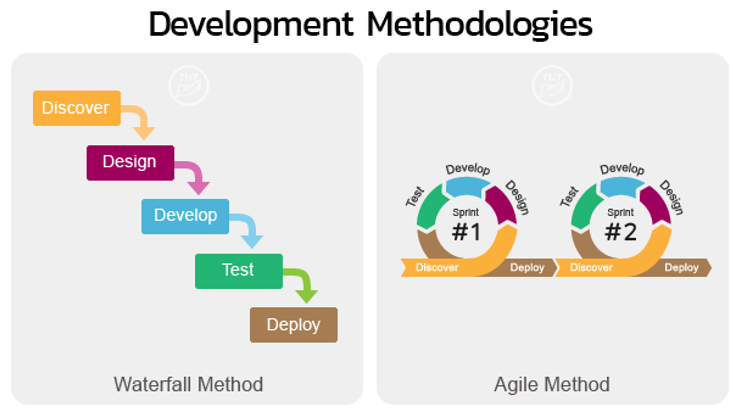
\includegraphics[scale=0.6]{agile}
		\caption{ความแตกต่างระหว่าง Waterfall Method กับ Agile Method}
		\end{figure}
	\FloatBarrier
	\item Scrum (สกรัม) คือการนำแนวคิดในการทำงานแบบ Agile (อไจล์) มาปฏิบัติตามขั้นตอนของสกรัม เพื่อระบุปัญหาที่มีความซับซ้อน เปลี่ยนแปลงบ่อย เพื่อให้สามารถส่งมอบผลิตภัณฑ์ที่ตอบสนองต่อการเปลี่ยนแปลงที่เกิดขึ้นได้อย่างรวดเร็ว
ช่วยให้การพัฒนาผลิตภัณฑ์แบบ Agile มีขั้นตอนการการดำเนินงานและผลลัพธ์ที่ชัดเจน โปร่งใส สามารถตรวจสอบประสิทธิภาพของแต่ละขั้นตอนการดำเนินงาน สามารถปรับปรุงและวัดผลการปรับปรุงที่เกิดขึ้นได้
	\item Kanban ที่มาเริ่มต้นมาจากระบบการทำงานของ Toyota ซึ่งประสบความสำเร็จอย่างมากจนทำให้สามารถผลิตรถออกมาได้ไวกว่าคู่แข่งทั่วโลกจนครองตลาดไปได้มาก สำหรับวงการ Software ได้ถูก David J. Anderson จับนำมาปรับปรุงให้เข้ากับ Software Development เพื่อการพัฒนา Software ได้อย่างรวดเร็วที่สุดด้วยเช่นกัน และสุดท้ายถูกนำไปเป็นส่วนหนึ่งของ Lean Software Development รวมไปถึงถูกจัดให้เป็น Agile อีกแบบหนึ่งนอกเหนือไปจาก Scrum อีกด้วย
Kanban มีกฎอยู่แค่ 3 ข้อ 
	\begin{itemize}[leftmargin=0pt,itemindent=3cm]
		\item Visualize the workflow – แสดง flow การทำงานของระบบให้ออกมาให้เห็นภาพอย่างชัดเจน สามารถบอกได้ว่าขณะนี้งานไปติดขัดที่จุดไหน 			อย่างไรให้ชัดเจน
		\item Limit Work In Progress (WIP) – จุดหลักของ Kanban เลยคือการ limit งานต่อหนึ่งหน่วยย่อย เช่นงานสำหรับ Development ห้ามถือเกิน	 			2 งานเพื่อป้องกันไม่ให้งาน Overload มากเกินไป และจะทำให้สูญเสียเวลาไปมากกว่าที่ควรจะเป็น
		\item Measure the lead time – วัดผลการทำงานและปรับปรุงให้ดียิ่งขึ้นไปอีก ตรงนี้จะเรียกว่า Cycle time หรือค่าเฉลี่ยที่ Card 1 							อันจะอยู่บนบอร์ดตั้งแต่เริ่มต้นไปจนถึงขึ้นบน production จริง
		\end{itemize}
	\end{itemize}
\end{enumerate}

\subsection{Smart Contract \cite{smartcontract}}
\tab Smart Contract หมายถึง กระบวนการทางดิจิทัล ที่กำหนดขั้นตอนการทำธุรกรรมโดยอัตโนมัติไว้ล่วงหน้า โดยไม่ต้องอาศัยตัวกลาง อย่างเช่น ธนาคาร ซึ่งการสร้าง Smart Contract ที่เป็นระบบอัตโนมัติอย่างเต็มรูปแบบ โดยคู่สัญญาทั้งสองฝ่ายจะมีการตกลงกันก่อนหน้านี้ ถึงขั้นตอน กลไก ในการทำรายการธุรกรรมดังกล่าว ซึ่งการพัฒนานี้ส่งผลกระทบต่อรูปแบบธุรกิจแบบดั้งเดิมของธนาคาร

\subsection{Non-Fungible Token (NFT) \cite{nft}}
\tab NFT ย่อมาจาก Non-Fungible Token เป็นชื่อเรียกของ Cryptocurrency ประเภทหนึ่ง เป็นสินทรัพย์ดิจิทัลที่มีเพียงชิ้นเดียวในโลก ไม่สามารถทำซ้ำหรือคัดลอกได้ ต่อให้มีการก๊อบปี้ไป แต่ต้นฉบับของจริงจะมีอยู่เพียงหนึ่งเดียวเท่านั้น ส่วนโทเคน NFT ก็เป็นเหมือนโฉนด เพื่อแสดงความเป็นเจ้าของสินทรัพย์ชิ้นนั้น

\subsection{พินัยกรรม  \cite{will}}
\tab พินัยกรรม หมายถึง การแสดงเจตนากำหนดการเผื่อตายซึ่งให้มีผลบังคับได้เมื่อถึงแก่ความตาย หรือถ้าเป็นภาษาพูดก็ได้แก่คำสั่งเสียของผู้ตาย โดยในการทำพินัยกรรม กฎหมายกำหนดรูปแบบไว้ 5 แบบด้วยกัน ดังนี้
\begin{enumerate}[label=\thesubsection.\arabic*,leftmargin=0pt,itemindent=2.5cm]
\item พินัยกรรมแบบธรรมดา ผู้ทำต้องทำเป็นหนังสือ คือการพิมพ์ข้อความพินัยกรรมลงในกระดาษ มากน้อยหรือจำนวนกี่แผ่นก็ต้องแล้วแต่เนื้อหาหรือจำนวนทรัพย์สิน   ลงวัน เดือน ปี ที่ทำให้ชัดเจน และผู้ทำต้องลงลายมือชื่อไว้ต่อหน้าพยานอย่างน้อย 2 คน และพยานต้องลงลายมือชื่อรับรองการทำพินัยกรรมในขณะทำด้วย
\item พินัยกรรมแบบเขียนเองทั้งฉบับ ผู้ทำพินัยกรรมจะทำเป็นเอกสารเขียนเองทั้งฉบับก็ได้ แต่ผู้ทำนั้นต้องเขียนพินัยกรรมนั้นด้วยลายมือตนเอง   ลงวัน เดือน ปีที่ทำ และที่สำคัญต้องลงลายมือชื่อผู้ทำด้วย กรณีนี้จะมีพยานมารับรู้การทำพินัยกรรมด้วยหรือไม่มีก็ได้
\item พินัยกรรมแบบเอกสารฝ่ายเมือง เป็นแบบพินัยกรรมที่ต้องอาศัยกระบวนการโดยเฉพาะที่มีเจ้าหน้าที่รัฐเข้ามาเกี่ยวข้อง   ผู้ทำพินัยกรรมต้องไปแจ้งความประสงค์โดยให้ถ้อยคำข้อความของตนแก่เจ้าพนักงานที่เขตหรืออำเภอพร้อมพยานอย่างน้อย 2 คน   เจ้าพนักงานจะอ่านข้อความให้ผู้ทำพินัยกรรมและพยานฟัง เมื่อเห็นว่าถูกต้องครบถ้วนแล้ว ผู้ทำพินัยกรรมพร้อมพยานทั้งสองต้องลงลายมือชื่อไว้   ต่อจากนั้น เจ้าพนักงานจะลงลายมือชื่อ วัน เดือน ปี ที่ทำ พร้อมประทับตราตำแหน่ง
\item พินัยกรรมแบบเอกสารลับ ผู้ทำพินัยกรรมทำพินัยกรรมแล้วปิดผนึก และนำไปที่ที่ทำการอำเภอหรือเขต   ผู้ทำพินัยกรรมต้องลงลายมือชื่อและพยานอีกอย่างน้อย 2 คน และให้ถ้อยคำต่อบุคคลเหล่านั้นว่าเป็นพินัยกรรมของตน   เจ้าหน้าที่จะบันทึกถ้อยคำลง วัน เดือน ปี ที่ทำพินัยกรรมแสดงไว้บนซองและประทับตราตำแหน่งไว้เป็นสำคัญโดยผู้ทำพินัยกรรม   พยานและเจ้าหน้าที่ต้องลงลายมือชื่อไว้หน้าซองตรงที่ปิดผนึก
\item พินัยกรรมแบบทำด้วยวาจา กรณีมีพฤติการณ์พิเศษที่บุคคลไม่สามารถทำพินัยกรรมแบบอื่นที่กล่าวมาข้างต้น เช่น การตกอยู่ในภยันตรายใกล้ความตาย หรืออยู่ในระหว่างสงคราม หรือเกิดมีโรคระบาด   เราสามารถทำพินัยกรรมแบบทำด้วยวาจาก็ได้ โดยผู้ทำพินัยกรรมต้องแสดงเจตนาทำพินัยกรรมต่อหน้าพยานอย่างน้อย 2 คนพร้อมกัน   พยานต้องรับฟังข้อความนั้นแล้วไปแจ้งต่อทางราชการโดยเร็วที่สุด ทั้งยังต้องแจ้งวัน เดือน ปี สถานที่ทำพินัยกรรมและพฤติการณ์พิเศษนั้นด้วย   เจ้าพนักงานต้องจดข้อความที่พยานแจ้งไว้ และพยาน 2 คนนั้นต้องลงลายมือชื่อไว้
\end{enumerate}
ข้อจำกัดและข้อควรระวังในการทำพินัยกรรม
\begin{enumerate}[label=\arabic*.,leftmargin=0pt,itemindent=2.5cm]
\item พินัยกรรมเป็นนิติกรรมที่ต้องทำตามแบบที่กำหนดเท่านั้น
\item ต้องเขียน วัน เดือน ปี ลงลายมือชื่อทั้งผู้ทำพินัยกรรมและผู้ที่เป็นพยาน
\item ผู้ที่เป็นพยานจะต้องไม่เป็นผู้เยาว์หรือผู้หย่อนความสามารถ และต้องไม่เป็นผู้มีส่วนได้เสียในกองมรดกนั้นด้วย
\item ผู้ทำพินัยกรรมต้องมีอายุ 15 ปีบริบูรณ์ขึ้นไป
\item พินัยกรรมควรจะตั้งผู้จัดการมรดกโดยสามารถระบุผู้ทำหน้าที่ผู้จัดการมรดกที่เจ้ามรดกไว้ใจลงในพินัยกรรมไปได้เลย
\item สิทธิ หน้าที่ และความรับผิดชอบ ก็สามารถกำหนดในพินัยกรรมได้
\item ทรัพย์สินที่ระบุในพินัยกรรมต้องเป็นทรัพย์สินหรือสิทธิของผู้ทำพินัยกรรมเท่านั้น ทั้งต้องแยกสินส่วนตัวออกจากสินสมรสด้วย
\item เงินประกันชีวิต เงินบำเหน็จตกทอด เงินมีบำนาญตกทอด เงินฌาปนกิจสงเคราะห์ตกทอด ไม่อาจเป็นมรดกที่ระบุลงในพินัยกรรมได้ เพราะไม่ใช่ทรัพย์ที่เจ้ามรดกมีอยู่ก่อนตาย

\section{งานวิจัยที่เกี่ยวข้อง}
\tab ในส่วนนี้เป็นการสรุปเนื้อหาโดยรวมของงานวิจัยที่เกี่ยวข้องกับการพัฒนาโครงงาน Will Chain Web application ที่มีการใช้งานในส่วนของ Digital Asset คือ CryptoWill
\subsection{CryptoWill  \cite{cryptowill}}
\tab โปรเจคนี้ได้อธิบายวิธีการทำระบบ CryptoWill ด้วยการให้ user ทำการเลือกเหรียญที่ต้องการทำ และใช้ Smart Contract ในการการส่งเหรียญให้ผู้รับและหลังจากนั้นตัวระบบจะทำการให้กำหนดเวลาของการ contract นี้จะส่งต่อเมื่อไหร่ อย่างเช่น ถ้าตั้ง 2 ปี ผู้ใช้งานจะต้องมาก่อนเวลาที่จะเกิด contract นี้ โดยรูปแบบของการทำจะมีวิธีการดำเนินการดังรูป

\begin{figure}[h]
	\centering
	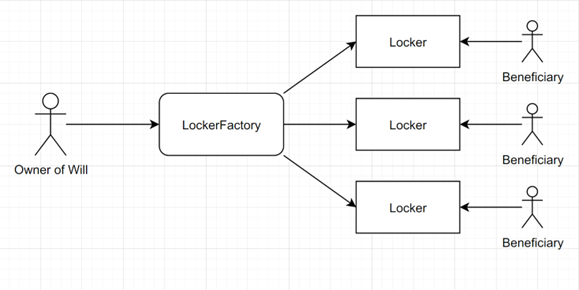
\includegraphics[scale=0.6]{CryptoWill}
	\caption{ภาพแสดงหลักการทำงานของโปรเจค CryptoWill}
\end{figure}

โดยเจ้าของพินัยกรรมจะทำพินัยกรรมและจะเก็บสินทรัพย์ไว้ใน blockchain และหลังจากนั้นจะส่งต่อให้ผู้รับไปเมื่อถึงเวลาของพินัยกรรมนั้น
\end{enumerate}

\clearpage

\section{เทคนิคและเทคโนโลยีที่ใช้}

\subsection{Ethereum Chain  \cite{eth}} 
\tab Ethereum คือแพลตฟอร์มบน Blockchain Network ที่่ทํางานด้วย Smart Contract มีลักษณะแพลตฟอร์มเป็นรูปแบบ Decentralized Platform แบบ Open Source ทําให้นักพัฒนาสามารถเข้ามาพัฒนา แก้ไข หรือดัดแปลงโค้ดได้ทุกคน พร้อมทั้งกําหนดเงื่อนไขต่าง ๆ สําหรับนําไปใช้งานบน Blockchain โดยมี Smart Contract ดําเนินการและระบบจะทํางานตามเงื่อนไขโปรแกรมที่กําหนดมา ทําให้ผู้ใช้งาน Blockchain ของ Ethereum ทําธุรกรรมได้ โดยไม่ต้องผ่านตัวกลางอื่น

\subsection{Etherscan  \cite{ethscan}} 
\tab Etherscan เป็นบล็อกสำรวจและแพลตฟอร์มการวิเคราะห์ที่ให้รายละเอียดเกี่ยวกับธุรกรรมบล็อคเชน Ethereum ที่กำลังรอดำเนินการ หรือได้รับการยืนยัน

\subsection{GitHub  \cite{github}}
\tab Git คือ Version Control ที่ถูกพัฒนาขึ้นมาเพื่อใช้ใ้นกระบวนการพัฒนาซอฟต์แวร์ คือ ระบบที่ถูกพัฒนาขึ้นมาเพื่อใช้สำหรับการติิดตาม ตรวจสอบ การพัฒนา แก้ไข Source Code ไฟล์ต่าง ๆ ในขั้นตอนการพัฒนา ที่สามารถตรวจสอบ ได้ทุกตัวอักษร ทุกบรรทัด ทุกไฟล์์ที่มีีการแก้ไข และยังมีคุณณลักษณะที่สนับสนุนการทำงานแบบ Agile อีกด้วย จึงทำให้เราสามารถทำงานได้อย่างมีประสิทธิภาพมากยิ่งขึ้น

\subsection{MetaMask \cite{metamask}}
\tab MetaMask หรือ MetaMask Wallet กระเป๋าเงินสินทรัพย์ดิจิทัล เป็น Wallet สำหรับเก็บ Cryptocurrency บนระบบนิเวศของ Ethereum ทุกชนิด ในกลุ่ม ERC-20 ซึ่ง Metamask พัฒนาโดยบริษัท ConsenSys โดยมีผู้ก่อตั้งคือ Joseph Lubin เมื่อปี 2016 (Joseph Lubin ยังเป็นผู้ร่วมก่อตั้ง Ethereum และ เคยยังเคยเป็น Speaker ในงาน Techsauce Global Summit)

\subsection{Next.js \cite{nextjs}}
\tab Next.js คือ JavaScript webapps framework ถูกสร้างขึ้น on top จาก library ดัง ๆ อย่าง React, Webpack, และ Babel และมีจุดเด่นที่ server-side rendering ที่สามารถ render หน้าเว็บบน server แทนที่จะ render บน browser ได้ จึงทำให้ข้อมูลที่ส่งให้ฝั่ง client นั้นถูก render เสร็จเรียบร้อยแล้ว ทำให้ฝั่ง client สามารถนำไปแสดงผลได้ทันที


\subsection{Tailwindcss \cite{tailwind}}
\tab Tailwindcss คือ CSS Utility Framework ที่ช่วยให้นักพัฒนาสร้าง UI ที่สำคัญได้ด้วยตัวเองอย่างรวดเร็ว และยังสามารถปรับแต่งในรายละเอียดปลีกย่อยได้ง่าย เนื่องจากมาพร้อมกับ Class สำเร็จรูปสุดอเนกประสงค์ที่ใช้งานได้ทันทีในกรณีที่ต้องการเปลี่ยน UI หลักของเฟรมเวิร์ก

\subsection{Figma \cite{figma}}
\tab Figma คือ เครื่องมือออกแบบเว็บไซต์ หรือ แอปฯ ต่างๆที่เกิดมาเพื่อช่วยนักออกแบบ UX/UI อย่างเราๆ โดยสามารถใช้งานได้ผ่านทาง web browser ทำให้สะดวกในการใช้งาน โดยตัวเครื่องมือออกแบบมาให้เหมาะกับคนที่จำเป็นจะต้องทำโปรเจกต์ร่วมกันกับทีม! เพราะสามารถแก้ไขงานร่วมกันได้แบบ real-time อีกทั้งตัวเครื่องมืที่ช่วยในการพัฒนาได้หลากหลายมากขึ้นอีกด้วย 

\subsection{DaisyUI \cite{daisyUI}}
\tab DaisyUI คือไลบรารีคอมโพเนนต์ CSS ที่ปรับแต่งได้ในแอปพลิเคชันส่วนหน้า DaisyUI ใช้คลาสยูทิลิตี้ CSS และ Tailwind โดยตรง โดยมุ่งเน้นที่การปรับแต่งและสร้างธีมสำหรับอินเทอร์เฟซผู้ใช้ ช่วยให้นักพัฒนา พัฒนาได้ง่ายขึ้น

\subsection{Solidity \cite{solidity}}
\tab Solidity คือภาษาสำหรับการสร้าง Smart Contract เป็นภาษาที่ได้รับอิทธิพลมาจาก C ++, Python และ JavaScript ที่สำคัญเลยก็คือเป็นภาษาชนิดที่ statically typed และเป็นภาษาแบบ Object Oriented (OO) เพราะว่ามีคุณสมบัติของการสืบทอดและการทำ struct เป็นต้น

\subsection{TypeScript \cite{typescript}}
\tab TypeScript เป็นภาษาโปรแกรมที่รวมความสามารถที่ ES2015 เองมีอยู่ สิ่งที่เพิ่มขึ้นมาคือสนับสนุน Type System รวมถึงคุณสมบัติอื่นๆที่เพิ่มมากขึ้น เช่น Enum และความสามารถที่เพิ่มขึ้นของการโปรแกรมเชิงวัตถุ TypeScript นั้นเป็น transpiler เหมือน Babel นั่นหมายความว่าตัวแปลภาษาของ TypeScript จะแปลโค๊ดที่เราเขียนให้เป็น JavaScript อีกทีนึง จึงมั่นใจได้ว่าผลลัพธ์สุดท้ายจะสามารถใช้งานได้บนเว็บเบราเซอร์ทั่วไป

\subsection{Wagmi \cite{wagmi}}
\tab Wagmi คือ library ที่จัดเก็บ React hook ที่ต้องใช้ในการพัฒนา Ethereum อย่างเช่น การเชื่อมต่อกระเป๋าดิจิทัล แสดงจำนวนเงิน และ การทำปฏิสัมพันธ์ระหว่าง Contract ได้

\subsection{Web3.js \cite{web3js}}
\tab Web3.js เป็น JavaScript API ที่ทําให้ส่วนติดต่อผู้ใช้งานสามารถติดต่อและเรียกใช้ฟังก์ชันจากฝั่งของ Ethereum ได้ โดย Web3.js สามารถส่ง API ไปติดต่อกับฝั่ง Smart Contract ให้สร้าง Transaction สําหรับเรียกใช้ Methods หรือ Get ค่าตัวแปรต่าง ๆ บน Smart Contract ที่อยู่บน Ethereum Blockchain ได้

\subsection{Hardhat \cite{hardhat}}
\tab Hardhat เป็น Development Environment ที่ทำให้เราสามารถพัฒนาตัว Smart Contract ได้โดย Hardhat สามารถทำ Compile, Deploy, Test, Debug ของตัว Smart contract และ สามารถ Test ตัว Smart Contract ได้บน Local Network ตัวเองได้

\subsection{Pinata \cite{pinata}}
\tab Pinata เป็น service management สำหรับจัดการ NFT ที่ช่วยให้ผู้ใช้สามารถโฮสต์ จัดการ และแชร์ไฟล์ประเภทใดก็ได้บนบล็อกเชนที่พวกเขาเลือกในการ IPFS pinning เพื่อทำการแชร์ไฟล์ต่อไปที่ IPFS global network ได้ง่ายขึ้น 

\subsection{IPFS \cite{ipfs}}
\tab IPFS เป็นเครือข่ายกระจายอำนาจแบบเพียร์ทูเพียร์ที่ช่วยให้ผู้ใช้สำรองไฟล์และเว็บไซต์โดยการโฮสต์ไว้บนโหนดจำนวนมาก ถูกสร้างขึ้นโดย Protocol Labs เป็นบริการที่อาศัยเครือข่ายคอมพิวเตอร์แบบกระจายที่โฮสต์เนื้อหา เช่น หน้าเว็บ ไฟล์ และแอปที่มิเรอร์ ซึ่งทั้งหมดนี้คุณสามารถดึงขึ้นมาได้โดยการป้อนลิงก์
Pinatas เป็นบริการโฮสต์ NFT ที่ใช้ IPFS เพื่อสำรองข้อมูลของสะสม crypto สำหรับคู่ค้าเช่น Rarible และ Sorare


\chapter{การออกแบบและวิธีการดำเนินงาน}
\tab เอกสารรายงานบทนี้จะกล่าวถึงระบบการทำงานของโครงงาน รวมถึงแผนภาพต่าง ๆ ที่ใช้อธิบายการทำงานในส่วนต่าง ๆ ของระบบ การออกแบบส่วนติดต่อผู้ใช้งาน (User Interface) ไดอะแกรมของระบบ รวมถึงขั้นตอนและวิธีการดำเนินงาน
\section{ระบบการทำงาน}
\subsection{ภาพรวมของระบบ}
\tab โดยภาพรวมของ Will Chain (Web application) จะประกอบไปด้วย 3 ส่วนหลักดังนี้
	\begin{figure}[h]
		\centering
		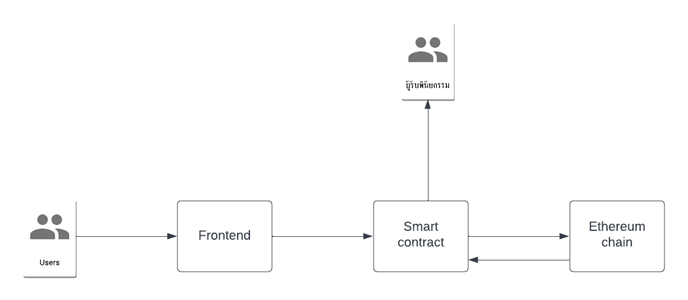
\includegraphics[scale=0.8]{Overall_system}
		\caption{ภาพรวมแสดงการทำงานของระบบ}
	\end{figure}
	
		\begin{itemize}
		\item ส่วนติดต่อผู้ใช้งานหรือ Frontend จะเป็นส่วนที่ผู้ใช้งานเห็น และใช้งาน
		\item Smart Contract จะเป็นส่วนที่ควบคุมการทำงานของระบบทั้งหมด โดยที่ผู้ใช้งานจะเข้าใช้งานผ่านทาง Frontend และจะส่งชุดคำสั่งมาเพื่อที่จะสั่งให้ Smart Contract นั้นทำงาน และจะส่งข้อมูลไปเก็บใน Blockchain ต่อไป
		\item Ethereum chain สำหรับเก็บข้อมูลการใช้งานของผู้ใช้งาน
	\end{itemize}

\subsection{User Journey}
	\begin{figure}[h]
		\centering
		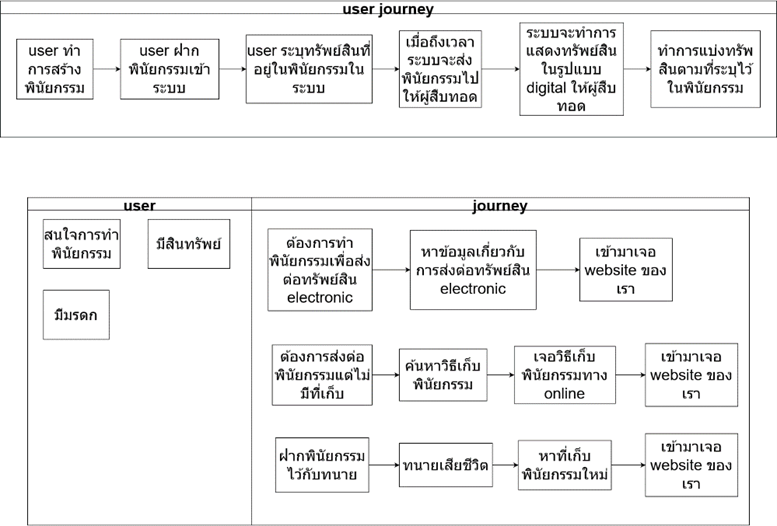
\includegraphics[scale=0.9]{UserJourney}
		\caption{แสดง User Journey}
	\end{figure}
\FloatBarrier
\hfill\\
\hfill\\
\hfill\\
\section{Crypto Wallet}
\tab ในการออกแบบระบบการทํางานของ Will Chain web application ได้เลือกใช้งาน Crypto Wallet ที่สามารถเชื่อมต่อกับ
Ethereum chain ได้ เพื่อที่จะทําให้สามารถทดสอบ และใช้งานจริงได้บน Ethereum chain โดย Crypto Wallet โดยเลือกใช้เป็น MetaMask Wallet

\section{Diagram Unified Modelling Language (UML)}
\tab หลังจากได้เขียนความต้องการ และฟังก์ชันแล้ว จึงทำการออกแบบและเขียนแผนภาพไดอะแกรมต่าง ๆ เพื่อให้สามารถเข้าใจระบบการทำงานมากยิ่งขึ้น โดยมีรายละเอียดดังนี้

\subsection{แผนภาพ Use Case Diagram}
	\begin{figure}[!htb]
		\centering
		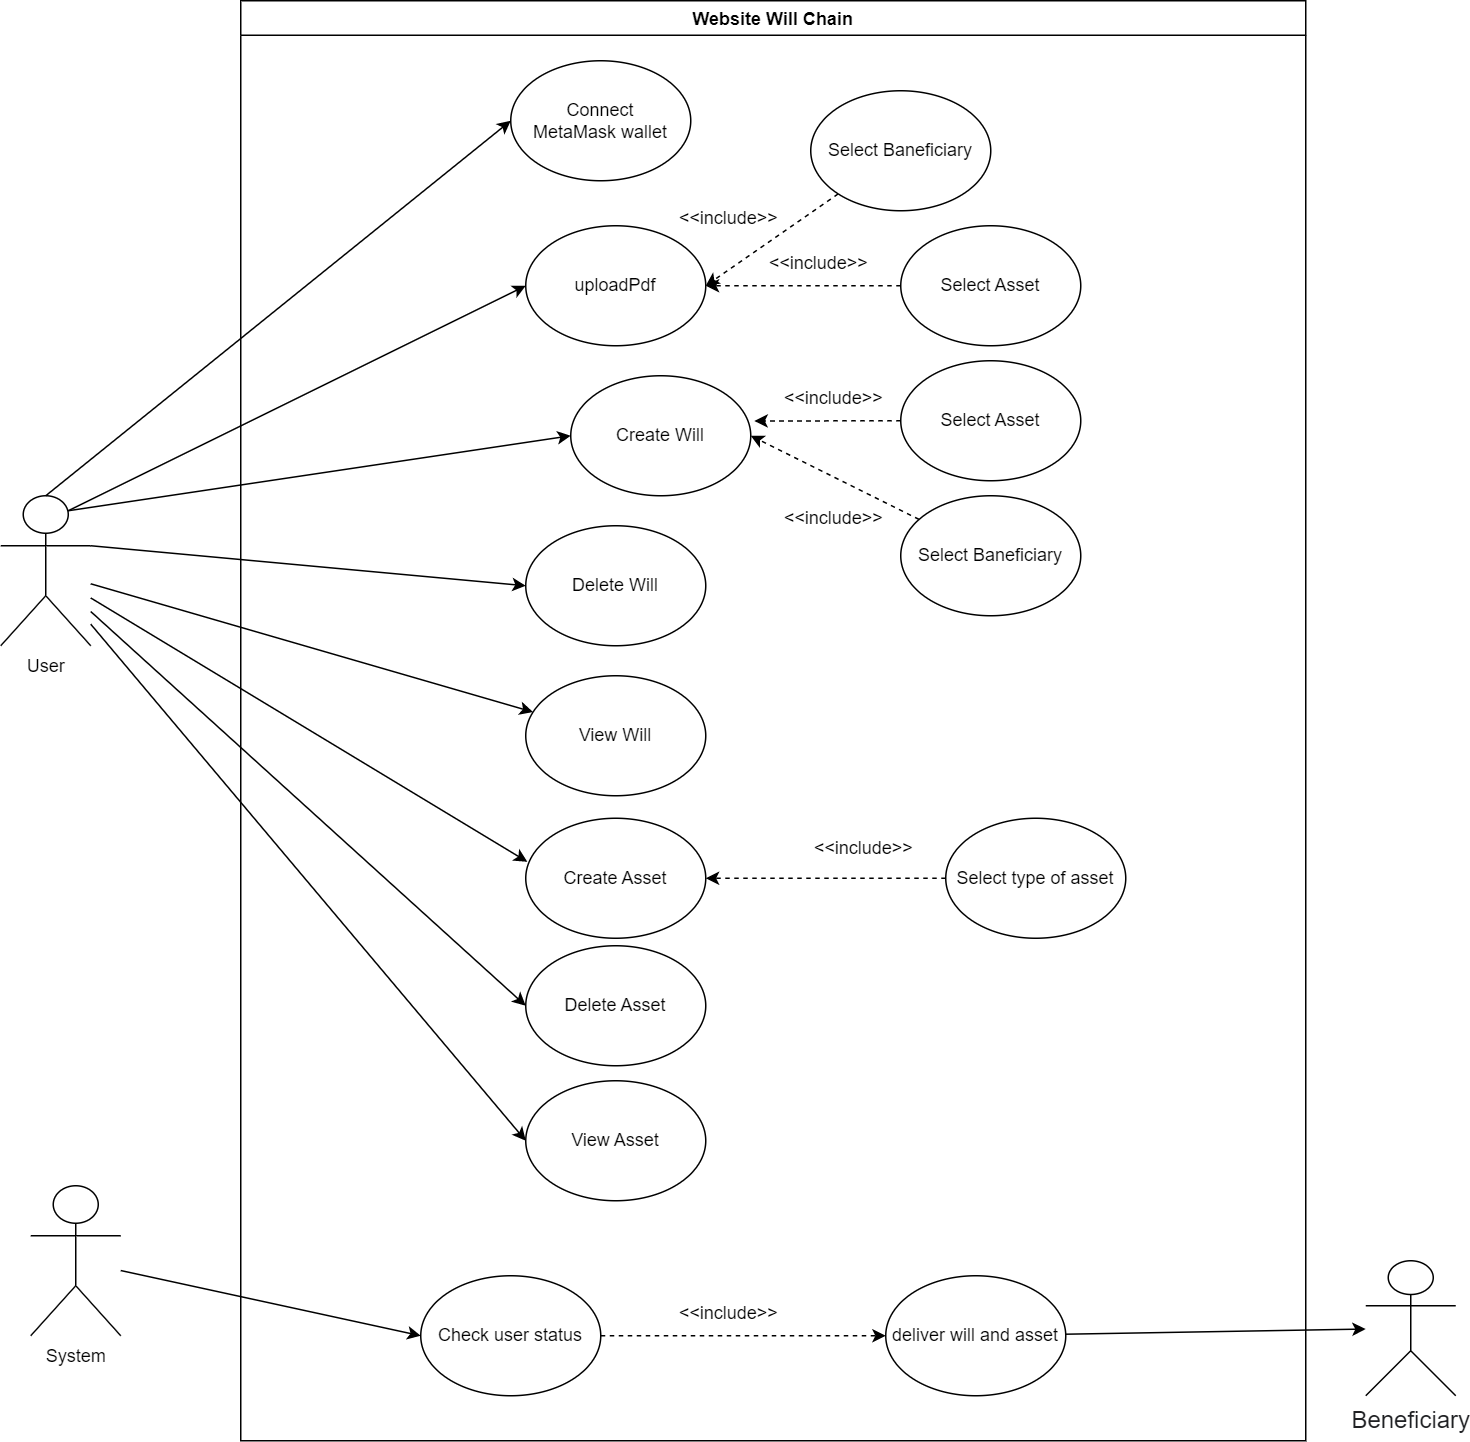
\includegraphics[scale=0.5]{UseCaseDiagram}
		\caption{แสดงการทำงานของระบบทั้งหมด Use Case Diagram}
	\end{figure}
\FloatBarrier

\tab จากรูปแสดง Use Case แสดงการทำงานของระบบทั้งหมดโดยจะมีผู้ใช้งาน (User) ที่ต้องการฝากพินัยกรรมไว้ในระบบทำการใช้งานระบบผ่าน platform ของ Will Chain Web application  โดยผู้ใช้งานจำเป็นต้องเชื่อมต่อกระเป๋าเงินอิเล็กทรอนิกส์ของ meta mask ก่อนหลังจากนั้นจึงจะสามารถ สร้าง,ลบหรือ upload พินัยกรรมพร้อมทั้งมีระบบจัดการทรัพย์สินที่ผู้ใช้แนบไว้พร้อมกับพินัยกรรม และจะมีระบบที่ทำการตรวจสอบสถานะของผู้ใช้งานเพื่นที่จะทำการส่งผ่านพินัยกรรมไปยังผู้รับผลประโยชน์เมื่อถึงเวลา   จากแผนภาพ Use Case Diagram ตามรูปที่ สามารถอธิบายรายละเอียดการทํา งานของแต่ละ Use Case ได้ดังต่อไปนี้ โดยจะกล่าวถึงในหัวข้อ Use Case Narrative ถัดไป
\clearpage

\subsection{Use Case Narrative}
\subsubsection{Use Case Connect Wallet}

\begin{table}[h]
\centering
\caption{ตารางแสดงรายละเอียดของ Use Case Connect MetaMask Wallet}
\begin{tabularx}{\textwidth}{|l|X|X|} 
\hline
Use Case Name:     & \multicolumn{2}{l|}{Connect MetaMask wallet}                                                                                                                                                                                                                       \\ 
\hline
Actors:            & \multicolumn{2}{l|}{User}                                                                                                                                                                                                                                          \\ 
\hline
Pre-Condition:     & \multicolumn{2}{l|}{User ต้องทำการสร้างกระเป๋าเงิน
  MetaMask}                                                                                                                                                                                                     \\ 
\hline
Post-Condition:    & \multicolumn{2}{l|}{กระเป๋าเงินเชื่อมต่อกับ
  Will Chain}                                                                                                                                                                                                            \\ 
\hline
Brief Description: & User                                                                                                        & System                                                                                                                                               \\ 
\hline
Flow of Event:     & \begin{tabular}[c]{@{}l@{}}1.เลือกเมนู Connect Wallet \\\\3.ยืนยันการเชื่อมต่อ MetaMask Wallet\end{tabular} & \begin{tabular}[c]{@{}l@{}}~ ~ ~ ~ \\2.รอผู้ใช้งานเลือก Account และยืนยันการเชื่อมต่อ \\~ ~\\4.เชื่อมต่อ MataMask Wallet กับ Platform\end{tabular}  \\ 
\hline
Exception:         & ~                                                                                                           &                                                                                                                                                      \\
\hline
\end{tabularx}
\end{table}

\FloatBarrier
\subsubsection{Use Case Create Will}
	\begin{table}[h]
\centering
\caption{ตารางแสดงรายละเอียดของ Use Case Create Will}
\begin{tabularx}{\textwidth}{|l|X|X|} 
\hline
Use Case Name:     & \multicolumn{2}{l|}{Create Will}                                                                                                                                                                                        \\ 
\hline
Actors:            & \multicolumn{2}{l|}{User}                                                                                                                                                                                               \\ 
\hline
Pre-Condition:     & \multicolumn{2}{l|}{User ต้องทำการเชื่อมบัญชีกับ MetaMask Wallet}                                                                                                                                                \\ 
\hline
Post-Condition:    & \multicolumn{2}{l|}{พินัยกรรมถูกบันทึกเข้าระบบ}                                                                                                                                                                         \\ 
\hline
Brief Description: & User                                                                                           & System                                                                                                                 \\ 
\hline
Flow of Event:     & \begin{tabular}[c]{@{}l@{}}1.เลือกเมนู Create Will \\~\\3.ยืนยันการสร้างพินัยกรรม\end{tabular} & \begin{tabular}[c]{@{}l@{}}~\\2.รอผู้ใช้งานกรอกรายละเอียดพินัยกรรมให้เสร็จ \\~\\4.บันทึกพินัยกรรมเข้าสู่ระบบ\end{tabular}  \\ 
\hline
Exception:         & ~                                                                                              &                                                                                                                        \\
\hline
\end{tabularx}
\end{table}
\FloatBarrier

\subsubsection{Use Case View Will}
	\begin{table}[h]
\centering
\caption{ตารางแสดงรายละเอียดของ  Use Case View Will}
\begin{tabularx}{\textwidth}{|l|X|X|} 
\hline
Use Case Name:     & \multicolumn{2}{l|}{View Will}                                                                                                                                                                                                                  \\ 
\hline
Actors:            & \multicolumn{2}{l|}{User}                                                                                                                                                                                                                       \\ 
\hline
Pre-Condition:     & \multicolumn{2}{l|}{User ต้องมีพินัยกกรรมที่ถูกสร้างไว้เรียบร้อยแล้ว}                                                                                                                                                                           \\ 
\hline
Post-Condition:    & \multicolumn{2}{l|}{ระบบทำการแสดงพินัยกรรมในระบบให้
  User}                                                                                                                                                                                     \\ 
\hline
Brief Description: & User                                                                                                              & System                                                                                                                      \\ 
\hline
Flow of Event:     & \begin{tabular}[c]{@{}l@{}}1.เลือกเมนู พินัยกรรมของฉัน \\\\3.เลือกพินัยกรรมที่อยู่ในระบบที่ต้องการดู \\~ ~\end{tabular} & \begin{tabular}[c]{@{}l@{}}2.ระบบทำการแสดงพินัยกรรมที่ถูกบันทึกในระบบ  \\\\4.ทำการแสดงพินัยกรรมที่ User เลือก\end{tabular}  \\ 
\hline
Exception:         & \multicolumn{2}{l|}{~}                                                                                                                                                                                                                          \\
\hline
\end{tabularx}
\end{table}
\FloatBarrier
\clearpage

\subsubsection{Use Case Create Willl}
\begin{table}[h]
	\centering
	\caption{ตารางแสดงรายละเอียดของ Use Case Create Will}
	\begin{tabularx}{\textwidth}{|l|X|X|} 
	\hline
	Use Case Name:     & \multicolumn{2}{l|}{Create Will}                                                                                                                                           \\ 
	\hline
	Actors:            & \multicolumn{2}{l|}{User}                                                                                                                                                  \\ 
	\hline
	Pre-Condition:     & \multicolumn{2}{l|}{User ต้องทำการเชื่อมบัญชีกับ MetaMask Wallet}                                                                                                   \\ 
	\hline
	Post-Condition:    & \multicolumn{2}{l|}{พินัยกรรมถูกบันทึกเข้าระบบ}                                                                                                                            \\ 
	\hline
	Brief Description: & User                                                                                           & System                                                                    \\ 
	\hline
	Flow of Event:     & \begin{tabular}[c]{@{}l@{}}1.เลือกเมนูบันทึกพินัยกรรม  \\2.กรอกฟอร์มเพื่อทำการบันทึกพินัยกรรม\end{tabular} & \begin{tabular}[c]{@{}l@{}}\\\\3.บันทึกพินัยกรรมเข้าสู่ระบบ\end{tabular}  \\ 
	\hline
	Exception:         & ~                                                                                              &                                                                           \\
	\hline
\end{tabularx}
\end{table}
\FloatBarrier

\subsubsection{Use Case Delete Willl}
	\begin{table}[h]
\centering
\caption{ตารางแสดงรายละเอียดของ Use Case Delete Will}
\begin{tabularx}{\textwidth}{|l|X|X|} 
\hline
Use Case Name:     & \multicolumn{2}{l|}{Delete Will}                                                                                                                                                                                                                                                          \\ 
\hline
Actors:            & \multicolumn{2}{l|}{User}                                                                                                                                                                                                                                                                 \\ 
\hline
Pre-Condition:     & \multicolumn{2}{l|}{User ต้องมีพินัยกกรมที่ถูกสร้างไว้เรียบร้อยแล้ว}                                                                                                                                                                                                                      \\ 
\hline
Post-Condition:    & \multicolumn{2}{l|}{พินัยกรรมถูกลบออกจากระบบ}                                                                                                                                                                                                                                             \\ 
\hline
Brief Description: & User                                                                                                                                                       & System                                                                                                                       \\ 
\hline
Flow of Event:     & \begin{tabular}[c]{@{}l@{}}1.เลือกเมนู Delete Will \\\\3.เลือกพินัยกรรมที่อยู่ในระบบ \\4.ลบพินัยกรรมในระบบ \\5.ยืนยันการลบพินัยกรรมในระบบ \\~\end{tabular} & \begin{tabular}[c]{@{}l@{}}\\2.ระบบทำการแสดงพินัยกรรมที่ถูกบันทึกในระบบ  \\\\\\\\6. ทำการนำพินัยกรรมออกจากระบบ\end{tabular}  \\ 
\hline
Exception:         & \multicolumn{2}{l|}{~}                                                                                                                                                                                                                                                                    \\
\hline
\end{tabularx}
\end{table}
\FloatBarrier

\subsubsection{Use Case View Beneficiary}
\begin{table}[h]
\centering
\caption{ตารางแสดงรายละเอียดของ Use Case View Beneficiary}
\begin{tabularx}{\textwidth}{|l|X|X|} 
\hline
Use Case
  Name:     & \multicolumn{2}{l|}{View Beneficiary}                                                                                                         \\ 
\hline
Actors:              & \multicolumn{2}{l|}{User}                                                                                                                      \\ 
\hline
Pre-Condition:       & \multicolumn{2}{l|}{ระบบต้องมีการเพิ่ม beneficiary แล้ว}                                                                           \\ 
\hline
Post-Condition:      & \multicolumn{2}{l|}{ระบบทำการแสดง beneficiary}                                                                                             \\ 
\hline
Brief
  Description: & User  & System                                                                                                                                   \\ 
\hline
Flow of Event:     & \begin{tabular}[c]{@{}l@{}}1.เลือกเมนู พินัยกรรมของฉัน \\\\3.เลือกพินัยกรรมที่อยู่ในระบบที่ต้องการดู \\~ ~\end{tabular} & \begin{tabular}[c]{@{}l@{}}2.ระบบทำการแสดงพินัยกรรมที่ถูกบันทึกในระบบ  \\\\\\4.ทำการแสดงพินัยกรรมที่แสดง Beneficiary \\ ของพินัยกรรมนั้น\end{tabular}  \\ 
\hline
Exception:           & \multicolumn{2}{l|}{~}                                                                                                                           \\
\hline
\end{tabularx}
\end{table}
\FloatBarrier
\clearpage

\subsubsection{Use Case Set Beneficiary}
\begin{table}[h]
\centering
\caption{ตารางแสดงรายละเอียดของ Use Case Set Beneficiary}
\begin{tabularx}{\textwidth}{|l|X|X|} 
\hline
Use Case
  Name:     & \multicolumn{2}{l|}{Set Beneficiary}                                                                                                         \\ 
\hline
Actors:              & \multicolumn{2}{l|}{User}                                                                                                                      \\ 
\hline
Pre-Condition:       & \multicolumn{2}{l|}{ระบบต้องสร้างพินัยกรรมก่อน}                                                                           \\ 
\hline
Post-Condition:      & \multicolumn{2}{l|}{ผู้รับพินัยกรรมถูกบันทึกเข้าสู่ระบบ}                                                                                             \\ 
\hline
Brief
  Description: & User  & System                                                                                                                                   \\ 
\hline
Flow of Event:     & \begin{tabular}[c]{@{}l@{}}1.เลือกพินัยกรรมที่ต้องการเพิ่ม beneficiary \\~\\3.เลือกเมนู Set Baneficiary\end{tabular} & \begin{tabular}[c]{@{}l@{}}~\\2.ระบบทำการแสดงพินัยกรรมที่ถูกบันทึกในระบบ  \\~~\\\\4.ระบบจะทำการบันทึก Beneficiary ของพินัยกรรม\\เข้าสู่ระบบ\end{tabular}  \\ 
\hline
Exception:           & \multicolumn{2}{l|}{~}                                                                                                                           \\
\hline
\end{tabularx}
\end{table}
\FloatBarrier

\subsubsection{Use Case View Asset}
\begin{table}[h]
	\centering
	\caption{ตารางแสดงรายละเอียดของ Use Case View Asset}
	\begin{tabularx}{\textwidth}{|l|X|X|} 
	\hline
	Use Case Name:     & \multicolumn{2}{l|}{View Asset}                                                                                                                                           \\ 
	\hline
	Actors:            & \multicolumn{2}{l|}{User}                                                                                                                                                  \\ 
	\hline
	Pre-Condition:     & \multicolumn{2}{l|}{ระบบต้องมีการเพิ่ม Asset แล้ว}                                                                                                   \\ 
	\hline
	Post-Condition:    & \multicolumn{2}{l|}{ระบบทำการแสดง Asset}                                                                                                                            \\ 
	\hline
	Brief Description: & User                                                                                           & System                                                                    \\ 
	\hline
Flow of Event:     & \begin{tabular}[c]{@{}l@{}}1.เลือกเมนู พินัยกรรมของฉัน \\\\3.เลือกพินัยกรรมที่อยู่ในระบบที่ต้องการดู \\~ ~\end{tabular} & \begin{tabular}[c]{@{}l@{}}2.ระบบทำการแสดงพินัยกรรมที่ถูกบันทึกในระบบ  \\\\4.ทำการแสดงสินทรัพย์ที่อยู่ในพินัยกรรมนั้น\end{tabular}  \\ 
	\hline
	Exception:         & ~                                                                                              &                                                                           \\
	\hline
\end{tabularx}
\end{table}
\FloatBarrier

\subsubsection{Use Case Add Asset}
\begin{table}[h]
	\centering
	\caption{ตารางแสดงรายละเอียดของ Use Case Add Asset}
	\begin{tabularx}{\textwidth}{|l|X|X|} 
	\hline
	Use Case Name:     & \multicolumn{2}{l|}{Add Asset}                                                                                                                                           \\ 
	\hline
	Actors:            & \multicolumn{2}{l|}{User}                                                                                                                                                  \\ 
	\hline
	Pre-Condition:     & \multicolumn{2}{l|}{User ต้องทำการ upload พินัยกรรมเข้าสู้ระบบ}                                                                                                   \\ 
	\hline
	Post-Condition:    & \multicolumn{2}{l|}{พินัยกรรมถูกบันทึกเข้าระบบ}                                                                                                                            \\ 
	\hline
	Brief Description: & User                                                                                           & System                                                                    \\ 
	\hline
	Flow of Event:     & \begin{tabular}[c]{@{}l@{}}1.เลือกเมนู Add Asset \\2.ทำการ upload สินทรัพย์\end{tabular} & \begin{tabular}[c]{@{}l@{}}\\\\3.บันทึกสินทรัพย์ไว้ในพินัยกรรม\end{tabular}  \\ 
	\hline
	Exception:         & ~                                                                                              &                                                                           \\
	\hline
\end{tabularx}
\end{table}
\FloatBarrier
\clearpage

\subsubsection{Use Case Check User Status}
\begin{table}[h]
\centering
\caption{ตารางแสดงรายละเอียดของ Use Case Check User Status}
\begin{tabularx}{\textwidth}{|l|X|X|} 
\hline
Use Case
  Name:     & \multicolumn{2}{l|}{Check user
  status}                                                                                                         \\ 
\hline
Actors:              & \multicolumn{2}{l|}{Controller}                                                                                                                      \\ 
\hline
Pre-Condition:       & \multicolumn{2}{l|}{ระบบต้องทำการเชื่อม
  API กับเว็บไซต์กรมการปกครอง}                                                                           \\ 
\hline
Post-Condition:      & \multicolumn{2}{l|}{ระบบทำการตรวจสอบสถาณะของ
  User}                                                                                             \\ 
\hline
Brief
  Description: & User  & System                                                                                                                                   \\ 
\hline
Flow of Event:     & \begin{tabular}[c]{@{}l@{}}1.Controller ตรวจสอบสถาณะของผู้ทำพินัยกรรม\\จาก API กรมการปกครอง  \\~ ~\end{tabular} & \begin{tabular}[c]{@{}l@{}}\\\\\\2.ระบบทำการเช็คว่าการเสียชีวิตใช่ผู้ที่ทำพินัยกรรม\\ในระบบของเราหรือไม่  \\\\3. ทำการแสดงสถานะการเสียชีวิต\end{tabular}  \\ 

\hline
Exception:           & \multicolumn{2}{l|}{~}                                                                                                                           \\
\hline
\end{tabularx}
\end{table}
\FloatBarrier

\subsubsection{Use Case Active Will}
\begin{table}[h]
\centering
\caption{ตารางแสดงรายละเอียดของ Use Case Active Will}
\begin{tabularx}{\textwidth}{|l|X|X|} 
\hline
Use Case
  Name:     & \multicolumn{2}{l|}{ Active Wil}                                                                                                         \\ 
\hline
Actors:              & \multicolumn{2}{l|}{Controller}                                                                                                                      \\ 
\hline
Pre-Condition:       & \multicolumn{2}{l|}{ระบบต้องเช็คสถานะ User Status เป็น Active}                                                                           \\ 
\hline
Post-Condition:      & \multicolumn{2}{l|}{ระบบทำให้พินัยกรรมดำเนินการส่งต่อไปหา Beneficiary}                                                                                             \\ 
\hline
Brief
  Description: & User  & System                                                                                                                                   \\ 
\hline

Flow of Event:     & \begin{tabular}[c]{@{}l@{}}1.ทำการดำเนินการส่งพินัยกรรม \\ตามเลขบัตรประชาชนที่กำหนด  \\ \\~ ~\end{tabular} & \begin{tabular}[c]{@{}l@{}}2.ทำการส่งพินัยกรรมจากระบบไปหา Beneficiary \end{tabular}  \\ 
\hline
Exception:           & \multicolumn{2}{l|}{~}                                                                                                                           \\
\hline
\end{tabularx}
\end{table}
\FloatBarrier

\subsubsection{Use Case Claim Will}
	\begin{table}[h]
\caption{ตารางแสดงรายละเอียดของ Use Case Claim Will}
\begin{tabularx}{\textwidth}{|l|X|X|} 
\hline
Use Case
  Name:     & \multicolumn{2}{l|}{Claim Will}                                                                                                                                                                                       \\ 
\hline
Actors:              & \multicolumn{2}{l|}{User}                                                                                                                                                                                                         \\ 
\hline
Pre-Condition:       & \multicolumn{2}{l|}{ระบบทำการแจ้งเตือนว่าผู้ทำพินัยกรรมเสียชีวิตแล้ว}                                                                                                                                                                           \\ 
\hline
Post-Condition:      & \multicolumn{2}{l|}{ผู้รับผลประโยชน์เข้ามารับพินัยกรรมและสินทรัพย์}                                                                                                                                           \\ 
\hline
Brief
  Description: & User  & System                                                                                                                                                                                                                      \\ 
\hline
Flow of Event:     & \begin{tabular}[c]{@{}l@{}}1.เลือกเมนู Claim Will \\\\3.เลือกพินัยกรรมในระบบที่สามารถรับได้ \\ \\~ ~\end{tabular} & \begin{tabular}[c]{@{}l@{}}2.ระบบทำการแสดงพินัยกรรมที่ผู้รับผลประโยชน์\\สามารถรับได้  \\\\4.ทำการส่งพินัยกรรมและสินทรัพย์\\ให้ผู้รับผลประโยชน์\end{tabular}  \\ 
\hline
Exception:           & \multicolumn{2}{l|}{~}                                                                                                                                                                                                              \\
\hline
\end{tabularx}
\end{table}
\FloatBarrier


\clearpage
\subsubsection{Use Case Display Claim Asset}
	\begin{table}[h]
\caption{ตารางแสดงรายละเอียดของ Use Case Display Claim Asset}
\begin{tabularx}{\textwidth}{|l|X|X|} 
\hline
Use Case
  Name:     & \multicolumn{2}{l|}{Display Claim Asset}                                                                                                                                                                                       \\ 
\hline
Actors:              & \multicolumn{2}{l|}{Beneficiary}                                                                                                                                                                                                         \\ 
\hline
Pre-Condition:       & \multicolumn{2}{l|}{ระบบจะต้องมีพินัยกรรมที่ดำเนินการแล้ว}                                                                                                                                                                           \\ 
\hline
Post-Condition:      & \multicolumn{2}{l|}{แสดงสินทรัพย์จากพินัยกรรมที่สามารถรับได้}                                                                                                                                           \\ 
\hline
Brief
  Description: & User  & System                                                                                                                                                                                                                      \\ 
\hline
Flow of Event:     & \begin{tabular}[c]{@{}l@{}}1.เลือกเมนู Display Will  \\~ ~\end{tabular} & \begin{tabular}[c]{@{}l@{}}2.แสดงสินทรัพย์ที่ผู้รับผลประโยชน์ได้รับ\end{tabular}  \\ 
\hline
Exception:           & \multicolumn{2}{l|}{~}                                                                                                                                                                                                              \\
\hline
\end{tabularx}
\end{table}
\FloatBarrier
\clearpage


\subsection{Smart Contract}
	\begin{figure}[!thb]	
		\centering
		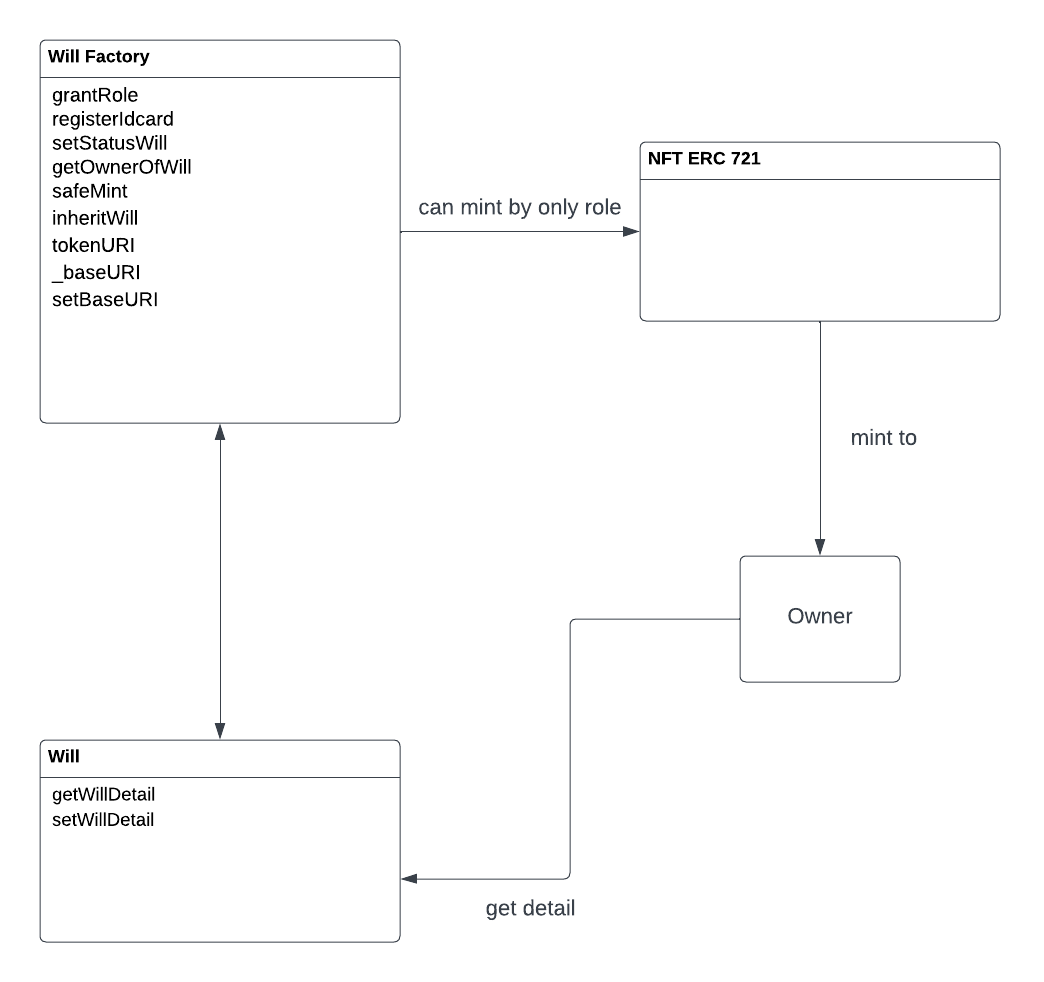
\includegraphics[scale=0.3]{smartContractDiagram}
		\caption{แสดงการ interaction ของ Smart Contract ของระบบ Will Chain}
	\end{figure}
	\FloatBarrier
\tab จากรูปแสดงการทำงานของตัว Smart Contract ของระบบ จะแบ่งเป็น 2 contract ที่ทำหน้าที่ต่างกันโดย Will factory จะทำหน้าที่เก็บข้อมูลของทุกพินัยกรรมและรวมถึงการจัดการพินัยกรรมของระบบทั้งหมดโดย Will factory สามารถทำการสร้างพินัยกรรมที่เป็น NFT ที่ใช้ ethereum standards ERC-721 และทำการ mint เก็บไว้ที่ตัวเจ้าของพินัยกรรมและเมื่อเกิดเหตุการณ์เสียชีวิตที่ได้รับจากระบบจะมีการ setStatusWill ให้เปลี่ยนเป็น active เพื่อที่จะทำการส่งต่อไปหาผู้รับพินัยกรรม ส่วน contract ต่อมาคือ will เป็น contract ที่ทำหน้าที่เกี่ยวกับจัดการมรดกของแต่ละพินัยกรรม โดยสามารถจัดการได้โดยเจ้าของพินัยกรรมว่าภายในพินัยกรรมของตัวเอง
\clearpage
\subsection{System Architecture Diagram}
	\begin{figure}[!thb]
		\centering
		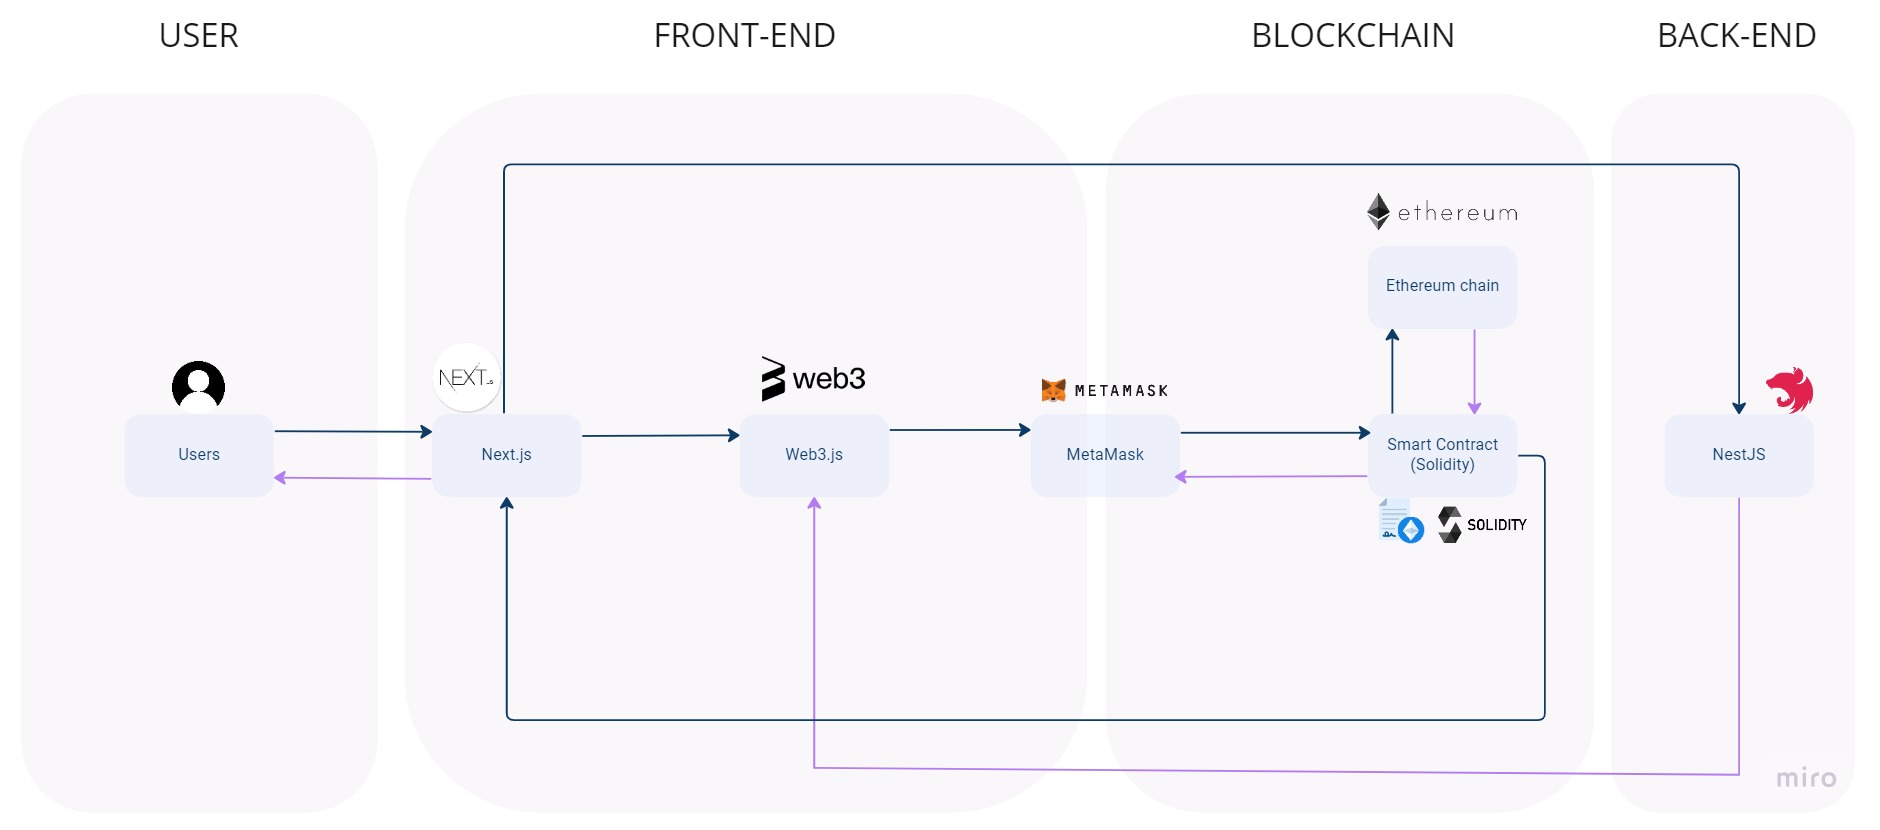
\includegraphics[scale=0.2]{systemArch}
		\caption{แสดงภาพออกแบบสถาปัตยกรรมของระบบ Will Chain}
	\end{figure}
	\FloatBarrier
ระบบของ Will Chain มีส่วนติดต่อกับระบบอื่น ๆ แยกตามประเภทดังนี้ \\
\textbf{Actor ของระบบ}
	\begin{itemize}
		\item User เป็นบุคคลที่ต้องการทำพินัยกรรมของ Will Chain
	\end{itemize}
\textbf{Front-end ของระบบ}
	\begin{itemize}
		\item Next.js จะทำหน้าที่แสดงผล UI ของเว็ปไซต์ Will Chain ในการทำพินัยกรรมต่าง ๆ 
		\item Web3.js จะทำหน้าที่ interact กับ method ต่าง ๆ ใน smart contract
		\item MetaMask จะทำหน้าที่เป็นตัว wallet สำหรับเก็บทรัพย์สินของเราและยังทำหน้าที่เป็นตัว login สำหรับใช้งานในระบบ
	\end{itemize}
\textbf{Blockchain ของระบบ}
	\begin{itemize}
		\item Smart contract จะทำหน้าที่คอยจัดการ transaction ภายใน Ethereum chain
		\item Deploy จะทำหน้าที่ deploy smart contract ขึ้นไปที่ ethereum chain
		\item Ethereum chain จะทำหน้าที่เก็บข้อมูล transaction และการทำพินัยกรรมต่าง ๆ ของระบบ
		\item Pinata จะทำหน้าที่เป็น gateway ในการใช้งาน storage ของระบบพินัยกรรม
	\end{itemize}
\textbf{Storage ของระบบ}
	\begin{itemize}
		\item IPFS จะทำหน้าที่เป็น storage ของระบบพินัยกรรม
	\end{itemize}
\clearpage
\subsection{Sequence Diagram}
	\subsubsection{Connect MetaMask}
		\begin{table}[h]
		\centering
		\caption{ตารางแสดงรายละเอียดของ Connect MetaMask Sequence Diagram}
		\begin{tabularx}{\textwidth}{|l|X|X|} 
			\hline
			Sequence Name: & Connect MetaMask                                                 \\ 
			\hline
			Actors:        & User                                                             \\ 
			\hline
			Pre-Condition: & User จะต้องทำการ Connect MetaMask เพื่อเป็นการ login ใช้งานระบบ  \\
			\hline
		\end{tabularx}
		\end{table}
		\begin{figure}[!thb]
			\centering
			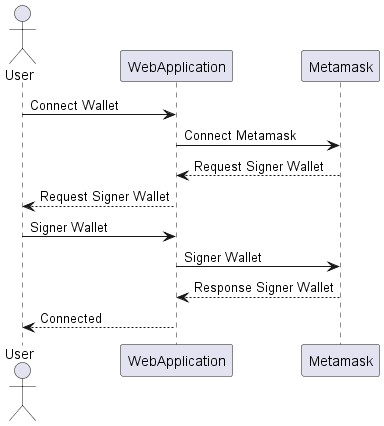
\includegraphics[scale=0.6]{connectMetamaskSeq}
			\caption{แสดง Connect MetaMask Sequence Diagram}
		\end{figure}
		\FloatBarrier
	\tab จากรูป จะเห็นได้ว่าเมื่อผู้ใช้งานทํางาน Connect MetaMask แล้วทาง Web Application จะไปเรียกใช้ MetaMask ที่ทําการติดตั้งไว้ใน Web browser ที่ทําการใช้งานอยู่ว่าขอทำการขอ Signer Wallet เพื่อทําการเชื่อมต่อ Web Application ซึ่งหลังจากทําการ Signer Walet จาก User แล้วตัว Metamask จะทำการ Connected กับ Web Application
\clearpage

	\subsubsection{Create Will}
		\begin{table}[h]
		\centering
		\caption{ตารางแสดงรายละเอียดของ Create Will Sequence Diagram}
		\begin{tabularx}{\textwidth}{|l|X|X|} 
			\hline
			Sequence Name: & Create Will                                                    \\ 
			\hline
			Actors:        & User                                                           \\ 
			\hline
			Pre-Condition  & User จะทำการ Create Will ที่เป็นการเขียนพินัยกรรมผ่านเว็ปไซต์  \\
			\hline
		\end{tabularx}
		\end{table}
		\begin{figure}[!thb]
			\centering
			\includegraphics[scale=0.45]{createWillseq}
			\caption{แสดง Create Will Sequence Diagram}
		\end{figure}
		\FloatBarrier
	\tab จากรูป ผู้ใช้เลือกใช้งาน Create Will จะแสดงหน้าจะแสดงฟอร์มสำหรับการทำพินัยกรรมผ่านระบบ จะทำการ Mint Will Token ไปที่ Metamask หลังจาก Mint NFT เสร็จสิ้นก็ทำการสร้าง Will Contract ที่จะทำหน้าจัดการสินทรัพย์หรือรายละเอียดพินัยกรรมต่าง ๆ ภายในพินัยกรรม หลังจากนั้นจะทำการแสดงผล Token id และ พินัยกรรม ที่ User มีอยู่ 
\clearpage

\subsubsection{View Will}
	\begin{table}[h]
	\centering
	\caption{ตารางแสดงรายละเอียดของ View Will Sequence Diagram}
\begin{tabularx}{\textwidth}{|l|X|X|} 
		\hline
		Sequence Name: & View Will                                  \\ 
		\hline
		Actors:        & User                                       \\ 
		\hline
		Pre-Condition  & User ต้องการดูรายละเอียดพินัยกรรมที่เขียน  \\
		\hline
	\end{tabularx}
	\end{table}
		\begin{figure}[!thb]
			\centering
			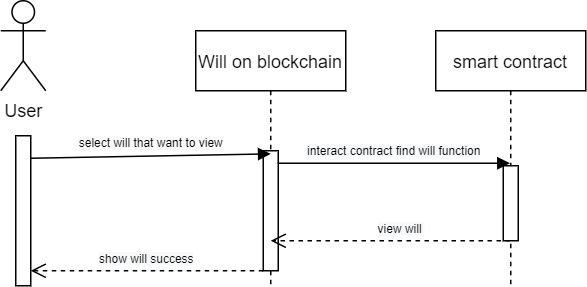
\includegraphics[scale=0.5]{viewWillseq}
			\caption{แสดง View Will Sequence Diagram}
		\end{figure}
		\FloatBarrier
	\tab จากรูป ผู้ใช้ทำการเลือกพินัยกรรมที่ต้องการจะแสดงโดยจะทำการเรียกใช้ฟังก์ชั่นเพื่อดูรายละเอียดใน Will Contract หลังจากนั้น Frontend จะเรียกใช้ฟังก์ชันแสดงสินทรัพย์ดิจิตอล และ เรียกใช้ฟังก์ชันแสดงสินทรัพย์จริง หลังจากนั้นจะทำการแสดงผลของรายละเอียดพินัยกรรม
	
\clearpage

\subsubsection{Upload Will}
		\begin{table}[h]
		\centering
		\caption{ตารางแสดงรายละเอียดของ Upload Pdf Will Sequence Diagram}
		\begin{tabularx}{\textwidth}{|l|X|X|} 
			\hline
			Sequence Name: & Upload Will                                             \\ 
			\hline
			Actors:        & User                                                        \\ 
			\hline
			Pre-Condition  & User จะทำการ Upload ที่เป็นการเขียนพินัยกรรมด้วยลายมือ  \\
			\hline
		\end{tabularx}
		\end{table}
		\begin{figure}[!thb]
			\centering
			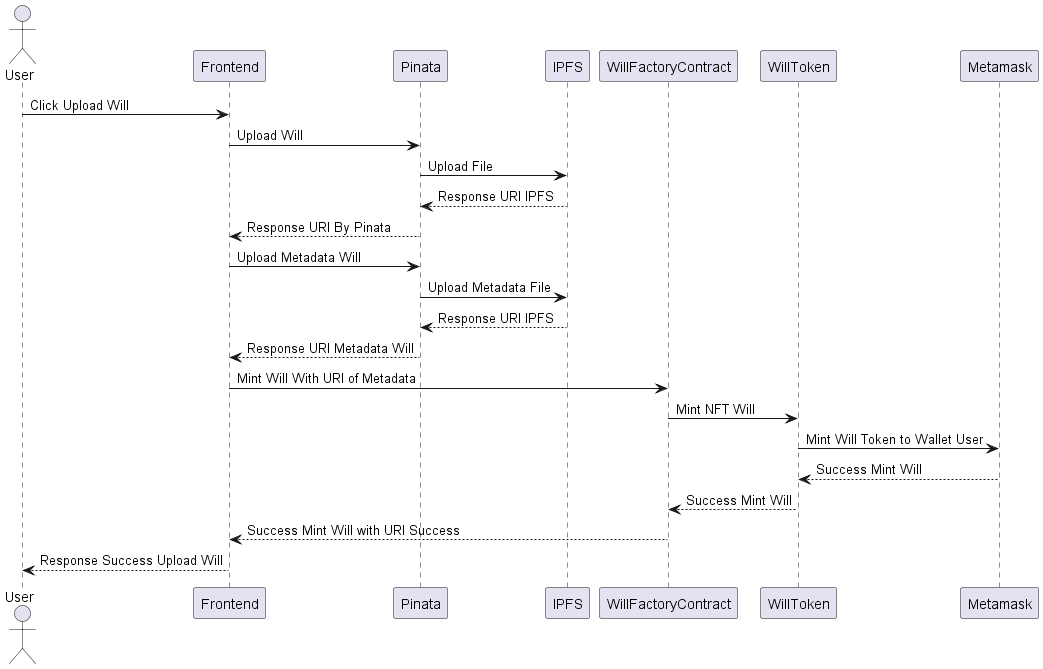
\includegraphics[scale=0.4]{uploadWillseq}
			\caption{แสดง Upload Will Sequence Diagram}
		\end{figure}
		\FloatBarrier
	\tab จากรูป ผู้ใช้เลือกใช้งาน Upload พินัยกรรมที่เขียนด้วยมือระบบจะแสดงฟอร์มที่ใช้สำหรับการ Upload พินัยกรรมไปที่ Pinata และ Pinata ทำหน้าที่ Upload File ไปที่ IPFS หลังจากนั้น IPFS จะส่ง URI ไปที่ Pinata จะทำการส่งต่อไปที่ Frontend หลังจากนั้น Upload Metadata Will หลังจากนั้น Pinata จะ Upload Metada Will ไปที่ IPFS หลังจากนั้น IPFS จะส่ง URI ไปที่ Pinata หลังจากนั้นส่งไป Frontend เพื่อทำการ mint Will Token ออกมาโดยสั่ง mint ไปที่ Will Factory Contract เพื่อทำการจัดการ Mint Will Token หลังจากนั้นจะทำการ Mint Will Token ไปที่ Metamask wallet ของ User หลังจากนั้น Frontend จะแสดงผลอัพโหลดพินัยกรรมเสร็จสิ้น
	
\clearpage

\subsubsection{Delete Will}
	\begin{table}[h]
		\centering
		\caption{ตารางแสดงรายละเอียดของ Delete Will Sequence Diagram}
		\begin{tabularx}{\textwidth}{|l|X|X|} 
			\hline
			Sequence Name: & Delete Will                           \\ 
			\hline
			Actors:        & User                                  \\ 
			\hline
			Pre-Condition  & User ต้องการที่จะลบพินัยกรรมที่เขียน  \\
			\hline
		\end{tabularx}
	\end{table}
		\begin{figure}[!thb]
			\centering
			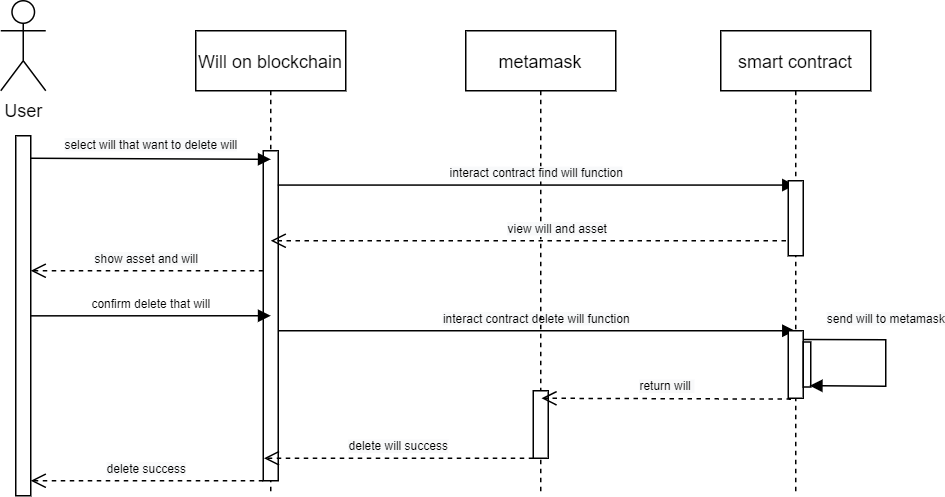
\includegraphics[scale=0.5]{deleteWillseq}
			\caption{แสดง Delete Will Sequence Diagram}
		\end{figure}
		\FloatBarrier
	\tab จากรูป ผู้ใช้ต้องการทำการลบ พินัยกรรมที่มีอยู่ในระบบ โดยระบบจะทำการ Burn Will Token ของเหรียญที่แทนพินัยกรรมนั้นหลังจากนั้นทำการลบพินัยกรรมที่ทำการเลือดไว้ใน WillFactoryContract หลังจากลบเสร็จสิ้นจะแสดงผลหน้าจอว่าลบพินัยกรรมสำเร็จ 
\clearpage

\subsubsection{View Beneficiary}
	\begin{table}[h]
	\centering
	\caption{ตารางแสดงรายละเอียดของ View Beneficiary Sequence Diagram}
	\begin{tabularx}{\textwidth}{|l|X|X|} 
		\hline
		Sequence Name: & View Beneficiary                                    \\ 
		\hline
		Actors:        & User                                                  \\ 
		\hline
		Pre-Condition  & User ต้องการดูผู้รับพินัยกรรมที่อยู่ระบบ \\
		\hline
		\end{tabularx}
	\end{table}
		\begin{figure}[!thb]
			\centering
			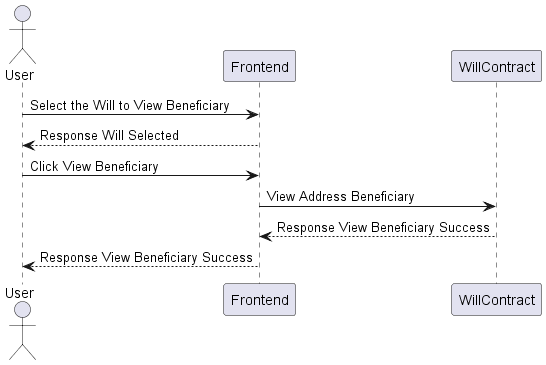
\includegraphics[scale=0.6]{viewBeneficiaryseq}
			\caption{แสดง View Beneficiary Sequence Diagram}
		\end{figure}
		\FloatBarrier
	\tab จากรูป ผู้ใช้ต้องเลือกพินัยกรรมที่ต้องการดูผู้รับพินัยกรรม และจะแสดงรายละเอียดพินัยกรรมหลังจากนั้นคลิกดูพินัยกรรมและ Frontend จะเรียกฟังก์ชั่นแสดงผู้รับพินัยกรรมจาก Will Contract หลังจากได้รับข้อมูลจาก Will Contract ตัว Frontend จะทำการแสดงผล Address ของ Beneficiary 
	
\clearpage

\subsubsection{Set Beneficiary}
	\begin{table}[h]
	\centering
	\caption{ตารางแสดงรายละเอียดของ Set Beneficiary Sequence Diagram}
	\begin{tabularx}{\textwidth}{|l|X|X|} 
		\hline
		Sequence Name: & Set Beneficiary                                  \\ 
		\hline
		Actors:        & User                                                  \\ 
		\hline
		Pre-Condition  & User ต้องการเลือกผู้รับพินัยกรรมที่อยู่ระบบ \\
		\hline
		\end{tabularx}
	\end{table}
		\begin{figure}[!thb]
			\centering
			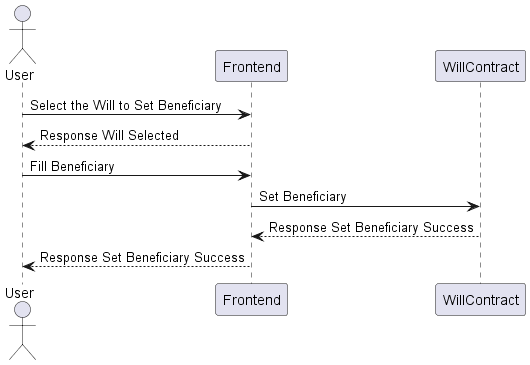
\includegraphics[scale=0.6]{setBeneficiaryseq}
			\caption{แสดง Set Beneficiary Sequence Diagram}
		\end{figure}
		\FloatBarrier
	\tab จากรูป ผู้ใช้ต้องเลือกพินัยกรรมที่ต้องการดูผู้รับพินัยกรรม และจะแสดงรายละเอียดพินัยกรรมหลังจากนั้นคลิกช่อง Beneficiary และใส่เลข Address ของ Beneficiary หลังจากนั้น Frontend จะทำการเรียกฟังก์ชัน setBeneficiary เพื่อทำการเพิ่มผู้รับพินัยกรรมใน will contract และหลังจากเพิ่มพินัยกรรมเสร็จสิ้นก็ทำการแสดงผลว่าเพิ่มผู้รับพินัยกรรมเสร็จสิ้น
	\clearpage
	
\subsubsection{View Assets}
	\begin{table}[h]
	\centering
	\caption{ตารางแสดงรายละเอียดของ View Assets Sequence Diagram}
	\begin{tabularx}{\textwidth}{|l|X|X|} 
		\hline
		Sequence Name: & View Assets                                \\ 
		\hline
		Actors:        & User                                                  \\ 
		\hline
		Pre-Condition  & User ต้องการดูสินทรัพย์ที่เชื่อมต่อ Smart
		  Contract  \\
		\hline
		\end{tabularx}
	\end{table}
		\begin{figure}[!thb]
			\centering
			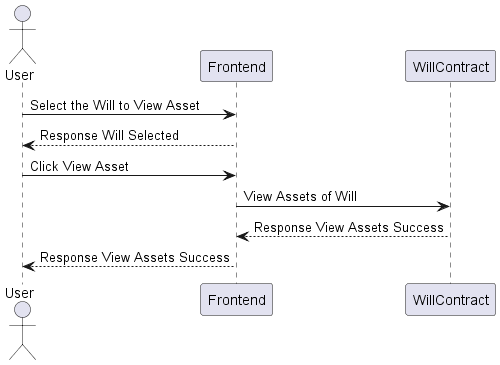
\includegraphics[scale=0.6]{viewAssetseq}
			\caption{แสดง View Assets Sequence Diagram}
		\end{figure}
		\FloatBarrier
	\tab จากรูป ผู้ใช้ต้องเลือกพินัยกรรมที่ต้องการดูผู้รับพินัยกรรม และจะแสดงรายละเอียดพินัยกรรมหลังจากนั้นคลิกดูสินทรัพย์และ Frontend จะเรียกฟังก์ชั่นแสดงสินทรัพย์จาก Will Contract หลังจากได้รับข้อมูลจาก Will Contract ตัว Frontend จะทำการแสดงผลสินทรัพย์เสร็จสิ้น
\clearpage

\subsubsection{Deposit Digital Assets}
	\begin{table}[h]
	\centering
	\caption{ตารางแสดงรายละเอียดของ Deposit Digital Assets Sequence Diagram}
	\begin{tabularx}{\textwidth}{|l|X|X|} 
		\hline
		Sequence Name: & Deposit Digital Assets                             \\ 
		\hline
		Actors:        & User                                                  \\ 
		\hline
		Pre-Condition  & User ต้องการเพิ่มสินทรัพย์ดิจิทัลที่เชื่อมต่อ Smart
		  Contract  \\
		\hline
		\end{tabularx}
	\end{table}
		\begin{figure}[!thb]
			\centering
			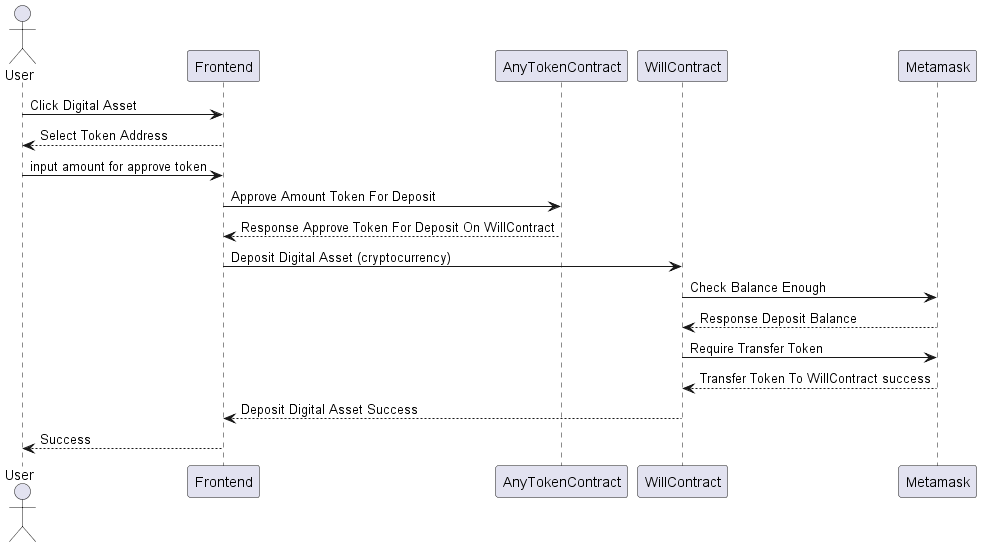
\includegraphics[scale=0.4]{depositDigitalseq}
			\caption{แสดง Deposit Digital Assets Sequence Diagram}
		\end{figure}
		\FloatBarrier
	\tab จากรูป ผู้ใช้ต้องการเพิ่มสินทรัพย์ดิจิทัลจะทำการคลิกเพื่อสินทรัพย์ดิจิทัลและทำการเลือกเหรียญที่ต้องการฝากไว้ในพินัยกรรมและ Frontend  จะทำการ Approve จำนวนของตัว Token นั้นที่จะทำการ Deposit เข้า Smart Contract หลังจากนั้น Frontend จะทำการ Deposit Digital Assets ไปที่ Will Contract และจะทำการเช็คยอดเงินคงเหลือใน Metamask ว่าเพียงพอต่อการฝากและหลังจากนั้นจะใช้ฟังก์ชั่นใน Will Contract Transfer เหรียญที่อยู่ใน Metamask ไปที่ Will Contract และหลังจากนั้น Frontend จะแสดงผลการเพิ่มสินทรัพย์ดิจิทัลเสร็จสิ้น
\clearpage

\subsubsection{Deposit Real Assets}
	\begin{table}[h]
	\centering
	\caption{ตารางแสดงรายละเอียดของ Deposit Real Assets Sequence Diagram}
	\begin{tabularx}{\textwidth}{|l|X|X|} 
		\hline
		Sequence Name: & Deposit Real Assets                          \\ 
		\hline
		Actors:        & User                                                  \\ 
		\hline
		Pre-Condition  & User ต้องการเพิ่มสินทรัพย์จริงที่เชื่อมต่อ Smart
		  Contract  \\
		\hline
		\end{tabularx}
	\end{table}
		\begin{figure}[!thb]
			\centering
			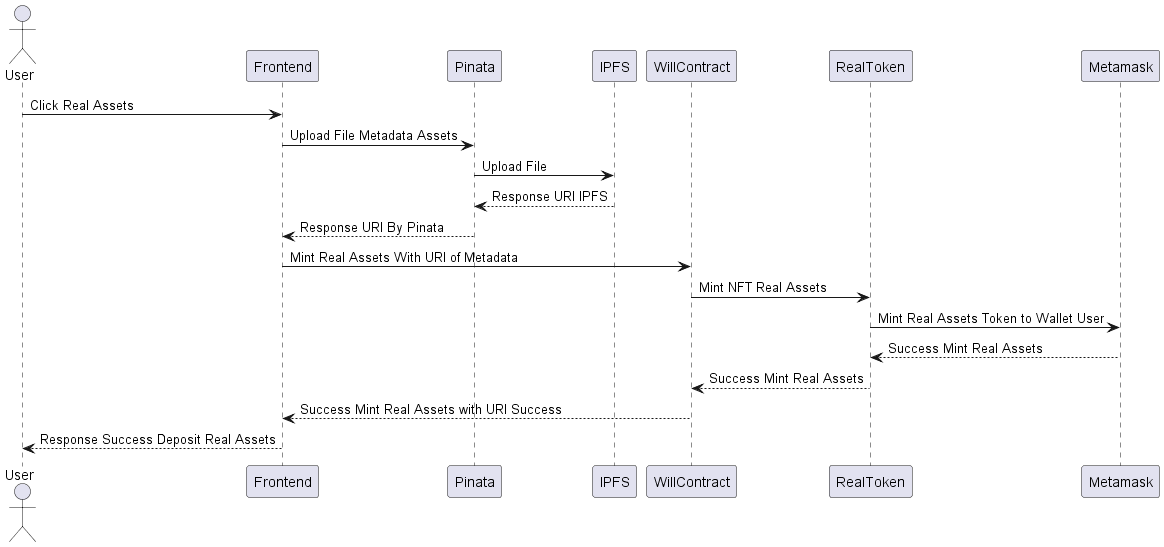
\includegraphics[scale=0.35]{depositRealseq}
			\caption{แสดง Deposit Real Assets Sequence Diagram}
		\end{figure}
		\FloatBarrier
	\tab จากรูป ผู้ใช้ต้องการเพิ่มสินทรัพย์จริงจะทำการคลิกเพื่อสินทรัพย์ดิจิทัล Frontend จะทำการอัพโหลด Metadata ของ Assets ไปที่ Pinata และ Pinata ทำหน้าที่ Upload File ไปที่ IPFS หลังจากนั้น IPFS จะส่ง URI ไปที่ Pinata จะทำการส่งต่อไปที่ Frontend หลังจากนั้น Frontend ทำการ mint Real Token ออกมาโดยสั่ง mint ไปที่ Will Contract เพื่อทำการจัดการ Mint Real Token หลังจากนั้นจะทำการ Mint Real Token ไปที่ Metamask wallet ของ User หลังจากนั้น Frontend จะแสดงผลเพิ่มสินทรัพย์จริงเสร็จสิ้น
\clearpage

\subsubsection{Active Will}
	\begin{table}[h]
\centering
\caption{ตารางแสดงรายละเอียดของ Active Will Sequence Diagram}
\begin{tabularx}{\textwidth}{|l|X|X|} 
\hline
Sequence Name: & Active Will                                          \\ 
\hline
Actors:        & Controller                                           \\ 
\hline
Pre-Condition  & ผู้กำกับพินัยกรรมต้องการเริ่มการสืบทอดพินัยกรรม  \\
\hline
\end{tabularx}
\end{table}
		\begin{figure}[!thb]
			\centering
			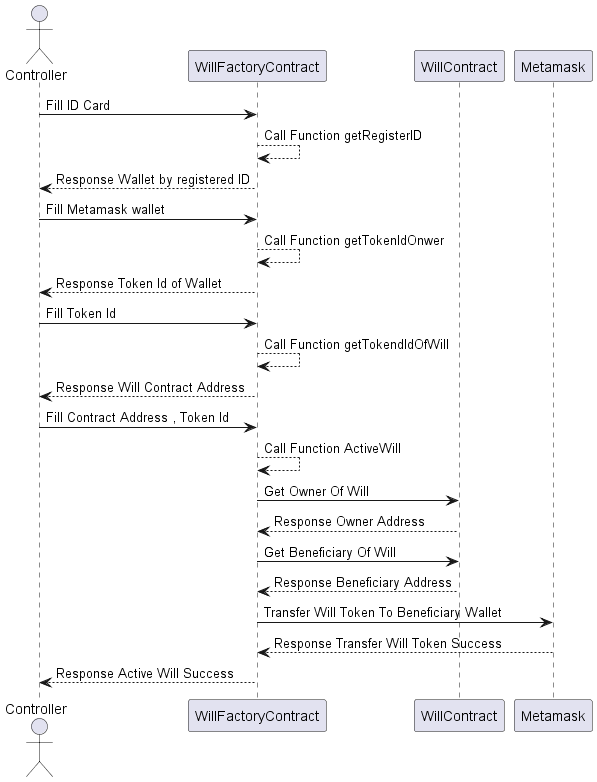
\includegraphics[scale=0.45]{activeWillseq}
			\caption{แสดง Active Will Sequence Diagram}
		\end{figure}
		\FloatBarrier
	\tab จากรูป ผู้ควมคุมจะทำการกรอกเลขบัตรประชาชน ไว้และเพื่อนำเลข Wallet Address ที่ทำการ register กับระบบไว้หลังจากนั้นจะกรอกเลขกระเป๋าเพื่อนำเลข Token id ที่เจ้าของพินัยกรรมถืออยู่มีอะไรบ้างหลังจากนั้น จะทำการกรอก token id เพื่อนำเลข Will Factory Contract address ไปทำการกรอกฟังก์ชั่น ActiveWill เพื่อทำการให้พินัยกรรมนี้สามารถทำงานได้ โดยจะใช้กระเป๋าของเจ้าของพินัยกรรมและกระเป๋าของผู้รับพินัยกรรม และทำการส่ง Will Token ไปที่ กระเป๋าของผู้รับพินัยกรรม
\clearpage	

\subsubsection{Claim Assets}
	\begin{table}[h]
\centering
\caption{ตารางแสดงรายละเอียดของ Claim Assets Sequence Diagram}
\begin{tabularx}{\textwidth}{|l|X|X|} 
\hline
Sequence Name: & Claim Asset                                             \\ 
\hline
Actors:        & Beneficiary                                            \\ 
\hline
Pre-Condition  & ทายาทจะทำการรับสินทรัพย์ที่ได้รับจากการเขียนพินัยกรรม  \\
\hline
\end{tabularx}
\end{table}
		\begin{figure}[!thb]
			\centering
			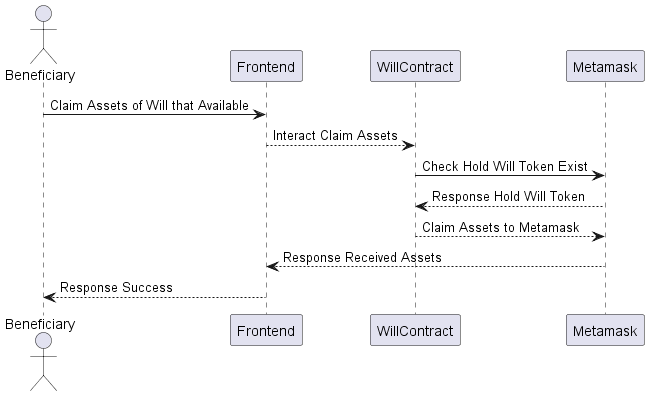
\includegraphics[scale=0.45]{claimAssetseq}
			\caption{แสดง Claim Assets Sequence Diagram}
		\end{figure}
		\FloatBarrier
	\tab จากรูป ทายาทจะรับสินทรัพย์ที่ได้รับจากการเขียนพินัยกรรมโดย Will Contract จะไปเช็ึคใน Metamask ว่า ลูกมี Will Token ที่สามารถ interact กับ Will Contract นี้ไหม หลังจากนั้นจะให้ผู้รับพินัยกรรมรับสินทรัพย์ที่อยู่ใน Will Contract ได้ไปที่ Metamask Wallet หลังจากนั้น Frontend จะแสดงผลรับสินทรัพย์เสร็จสิ้น
\clearpage


\section{ส่วนติดต่อผู้ใช้งาน (User Interface)}
\tab การออกแบบส่วนติดต่อผู้ใช้งาน โดยการออกแบบ Will Chain ได้คำนึงถึงการใช้งานของผู้ใช้งาน 
\subsection{หน้าแรก}
		\begin{figure}[!thb]
			\centering
			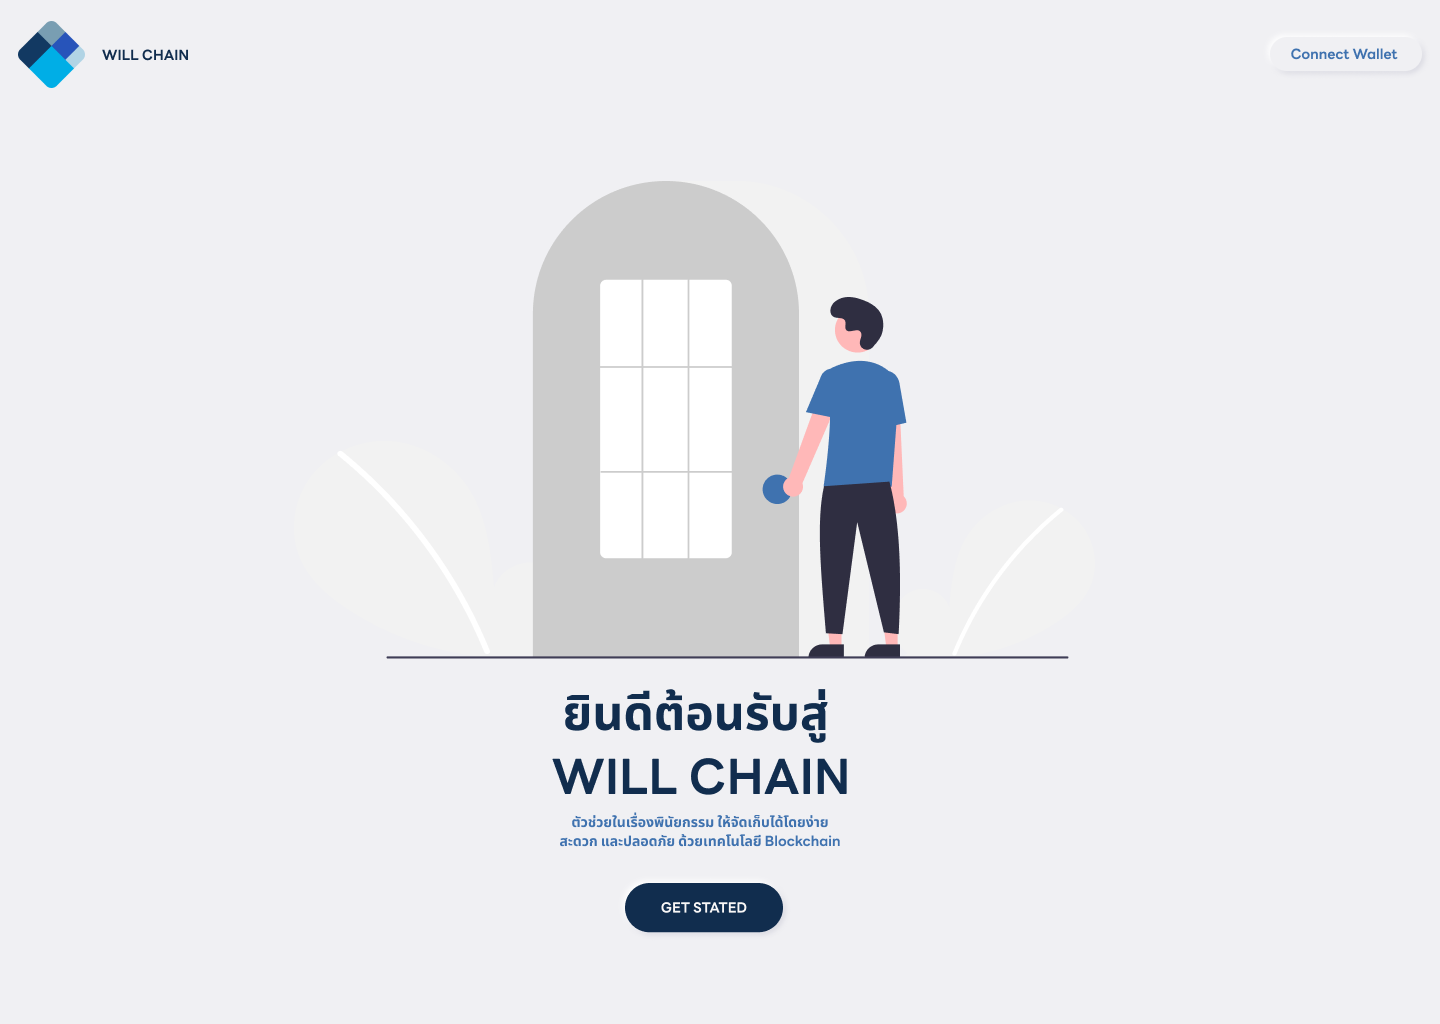
\includegraphics[scale=0.2]{Home}
			\caption{หน้าแรก}
		\end{figure}
		\FloatBarrier
		\tab จากรูป เป็นหน้าแรกของแพลตฟอร์ม Web application Will Chain ที่ยังไม่ได้ทำการเข้าสู่ระบบ โดยจะประกอบไปด้วยแนวคิดของแพลตฟอร์ม รวมไปถึงการเข้าถึงคู่มือการใช้งาน และยังสามารถกดที่ปุ่มแถบเมนูด้านขวาบนเพื่อเชื่อมต่อกับ MetaMask Wallet
\subsection{หน้าโปรไฟล์}
		\begin{figure}[!thb]
			\centering
			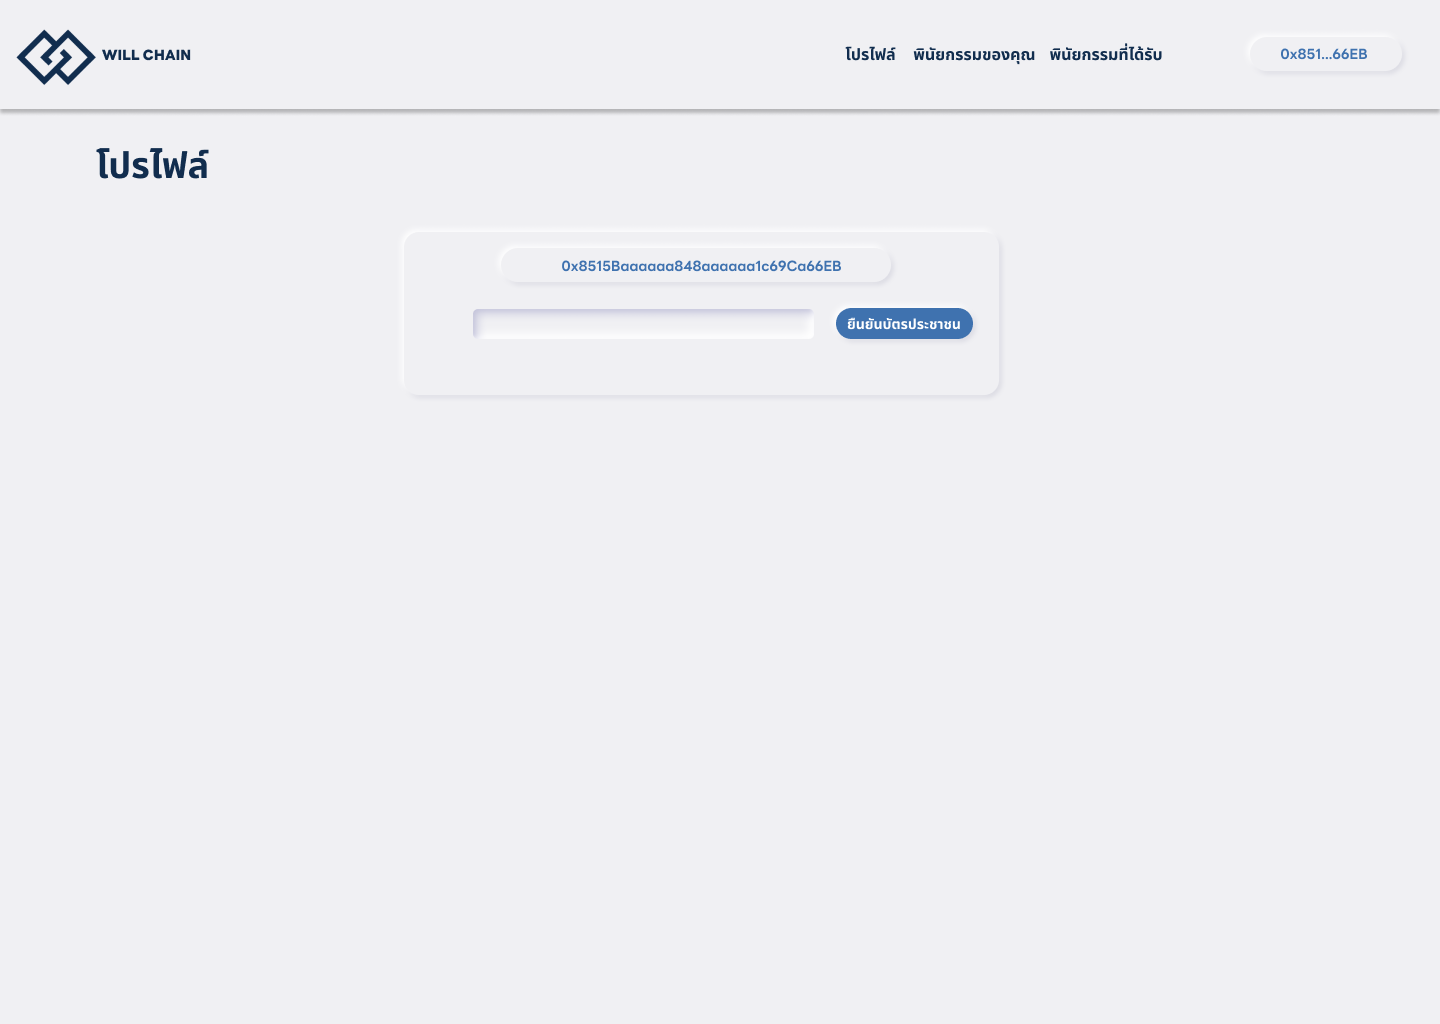
\includegraphics[scale=0.2]{profile}
			\caption{หน้าโปรไฟล์}
		\end{figure}
		\FloatBarrier
		\tab จากรูป เป็นหน้าโปรไฟล์จะต้องทำการเข้าสู่ระบบด้วย MetaMask Wallet โดยจะแสดงเลข Public key ทางด้านขวาบน โดยในหน้านี้จะแสดงเลข Public key ของ MetaMask Wallet และมีช่องสำหรับใส่เลขบัตรประชาชน และปุ่ม ''ยืนยันบัตรประชาชน'' เพื่อทำการยืนยันตัวตนสำหรับการใช้งานฟีเจอร์ต่าง ๆ ในระบบต่อไป
\subsection{หน้าโปรไฟล์ยืนยันการลงทะเบียน}
		\begin{figure}[!thb]
			\centering
			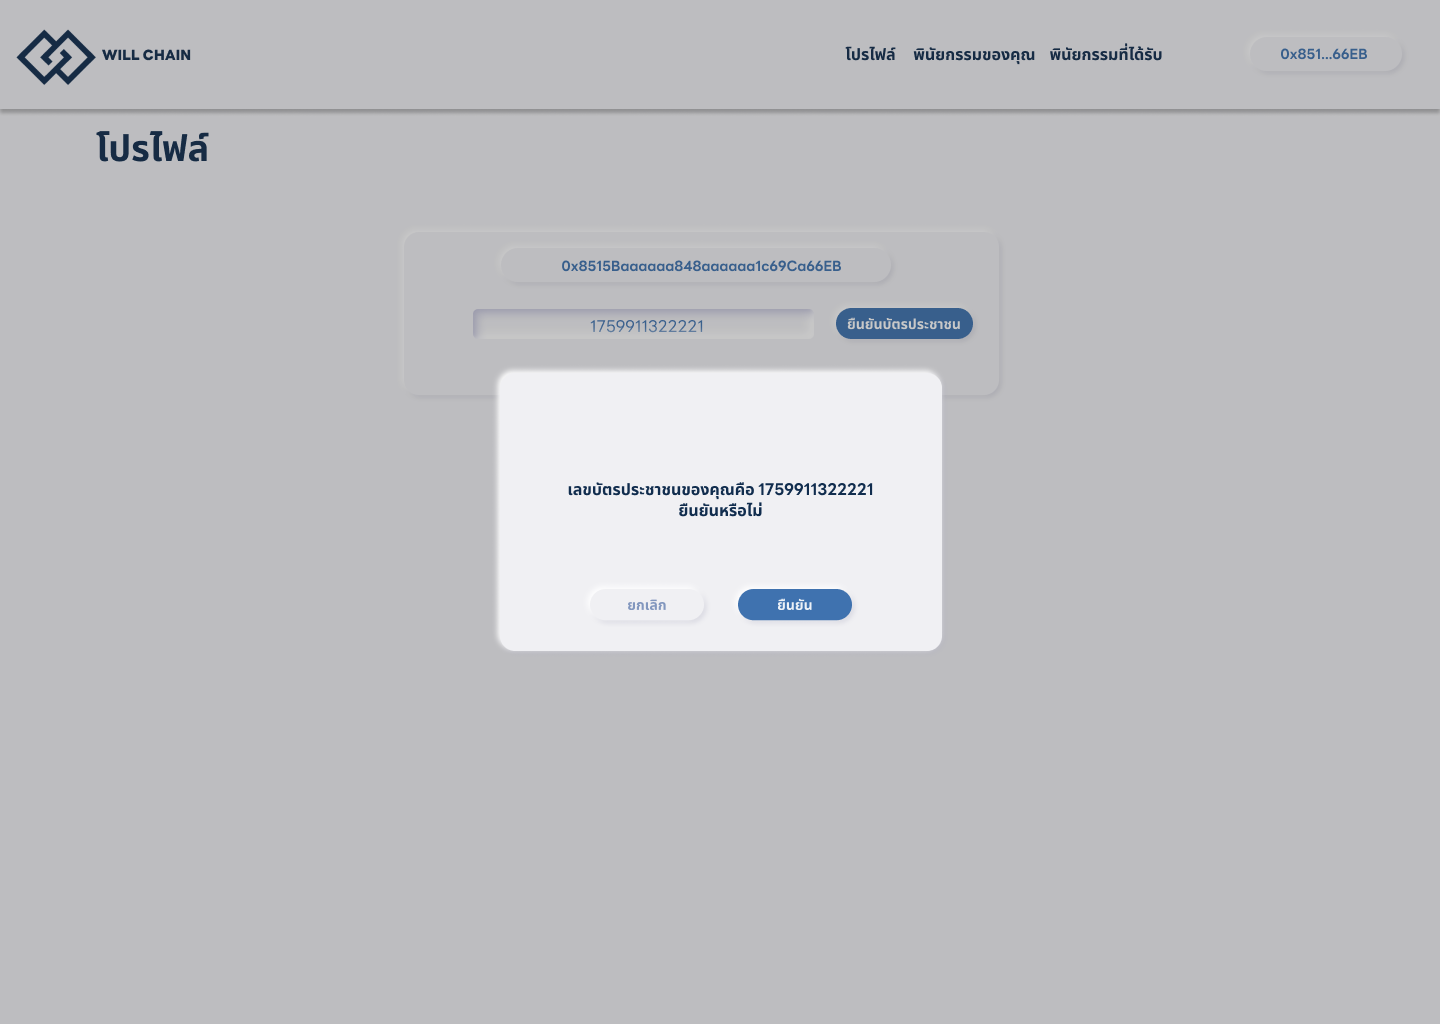
\includegraphics[scale=0.2]{profileConfirm}
			\caption{หน้าโปรไฟล์สำหรับการยืนยันการลงทะเบียนเลขบัตรประชาชน}
		\end{figure}
		\FloatBarrier
		\tab จากรูป เป็นหน้าโปรไฟล์ที่หลังจากกรอกเลขบัตรประชาชนเรียบร้อยแล้ว จะให้มีการยืนยันเพื่อตรวจสอบความถูกต้องอีกครั้งหนึ่ง
\subsection{หน้าโปรไฟล์ลงทะเบียนสำเร็จ}
		\begin{figure}[!thb]
			\centering
			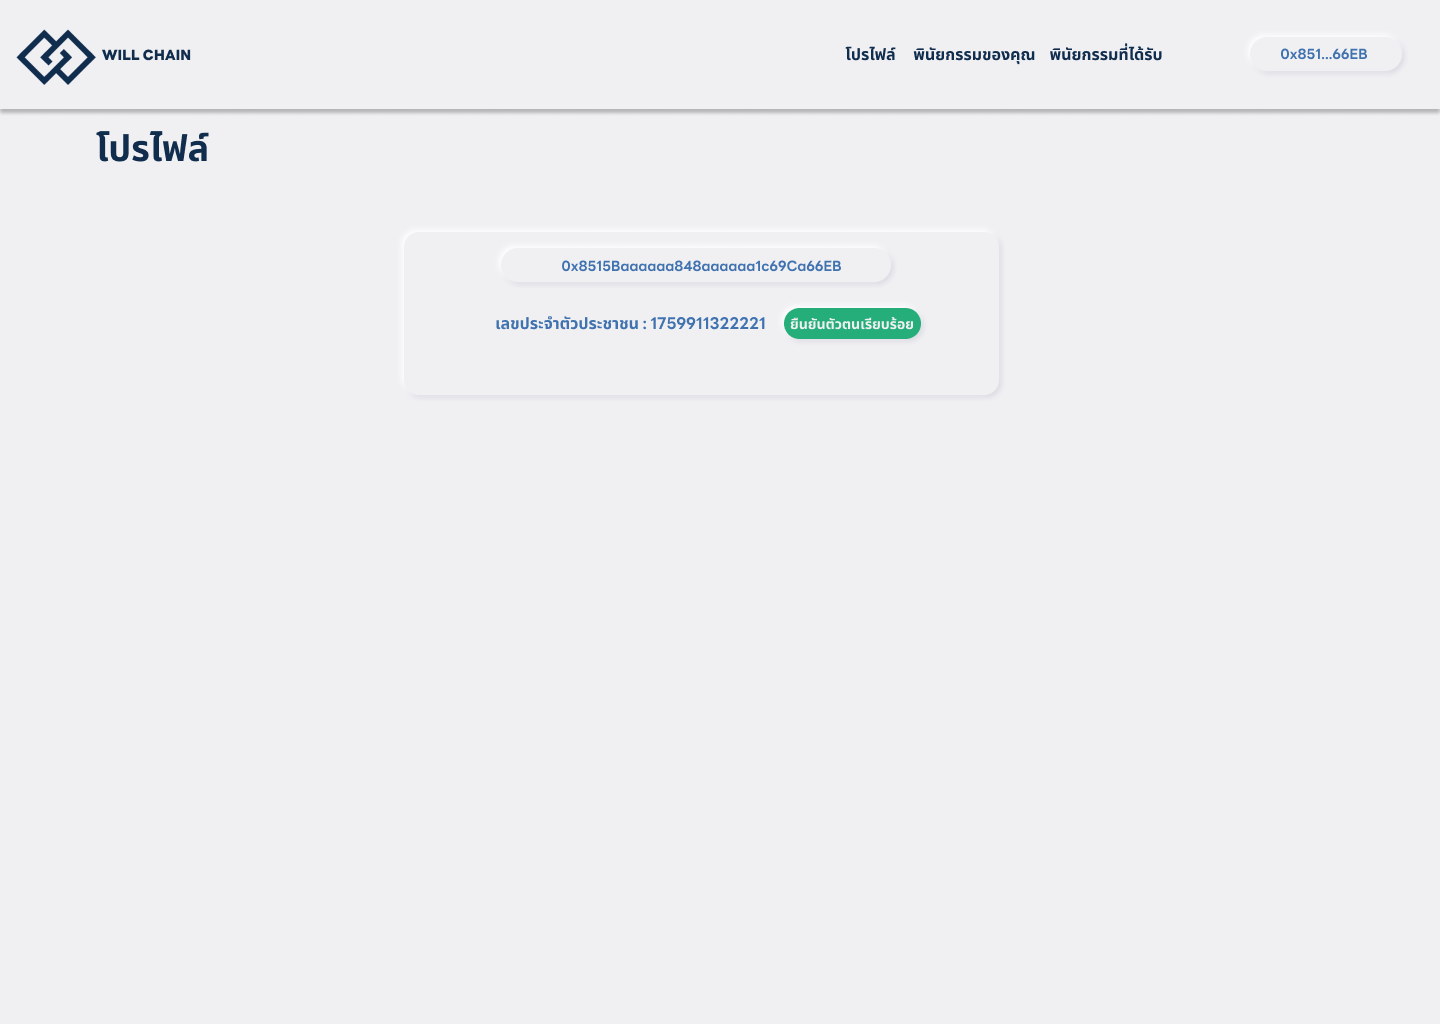
\includegraphics[scale=0.2]{profileSuccess}
			\caption{หน้าโปรไฟล์ ยืนยันการลงทะเบียนสำเร็จ}
		\end{figure}
		\FloatBarrier
		\tab จากรูป เป็นหน้าโปรไฟล์ที่เมื่อทำการกรอกการลงทะเบียนด้วยเลขบัตรประชาชนเสร็จสิ้น โดยจะมีปุ่มสีเขียว ''ยืนยันตัวตนเรียบร้อย'' เพื่อแสดงว่าทำการลงทะเบียนเลขบัตรประชาชนเรียบร้อยแล้ว
		
\clearpage
\subsection{หน้าพินัยกรรมของคุณ}
		\begin{figure}[!thb]
			\centering
			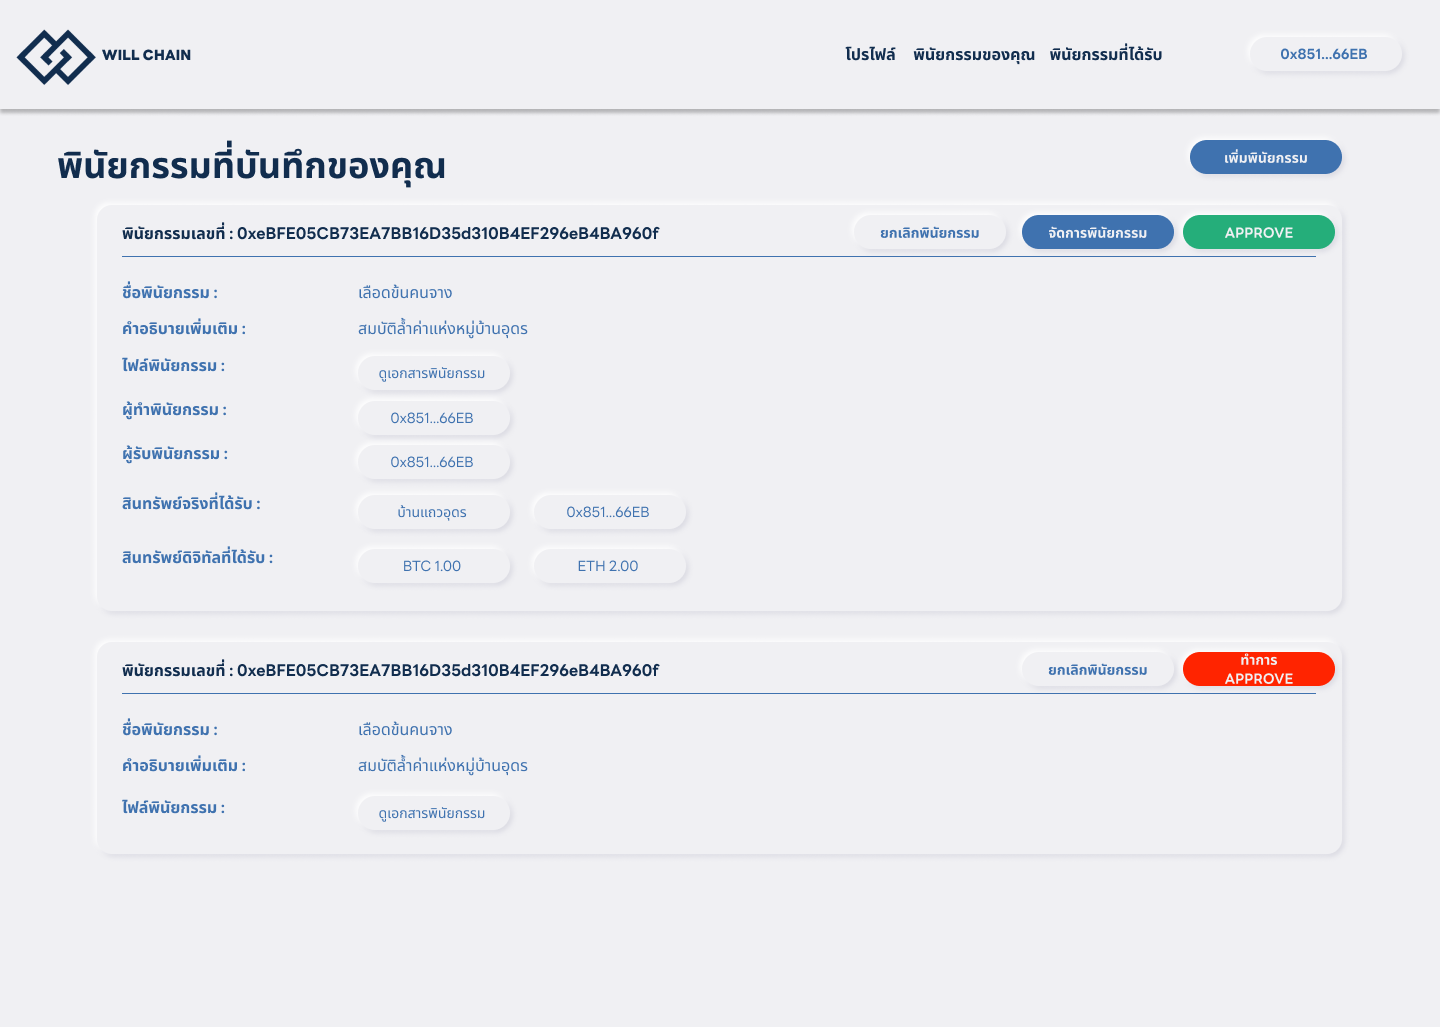
\includegraphics[scale=0.2]{userWill}
			\caption{หน้าพินัยกรรมของคุณ}
		\end{figure}
		\FloatBarrier
		\tab จากรูป เป็นหน้าพินัยกรรมที่บันทึกของคุณ จากการกดที่เมนู “พินัยกรรมของคุณ” ที่แถบเมนูด้านบน โดยที่ในหน้านี้จะแสดงพินัยกรรมที่มีอยู่ในระบบของผู้ใช้คนนี้ โดยที่ในหนึ่งพินัยกรรม จะแสดงเลขฉบับที่ของพินัยกรรม สถานะของพินัยกรรม และสามารถกดปุ่ม “ดูพินัยกรรม” เพื่อดูพินัยกรรมที่เป็นไฟล์ฉบับจริงได้ โดยในตารางด้านล่างนั้นจะแสดงผู้รับพินัยกรรม ต่อมาคือแสดงสินทรัพย์ทั้งหมดที่อยู่ในพินัยกรรมฉบับนี้ และแสดงสินทรัพย์จริง สุดท้ายคือแสดงสินทรัพย์ดิจิทัลทั้งหมดในพินัยกรรมนั้น และแสดงชนิดของสินทรัพย์ดิจิทัล  และสามารถกดปุ่ม “ลบพินัยกรรม” เพื่อลบพินัยกรรมนั้นออกจากระบบได้

\subsection{หน้ายกเลิกการทำพินัยกรรมของคุณ}
		\begin{figure}[!thb]
			\centering
			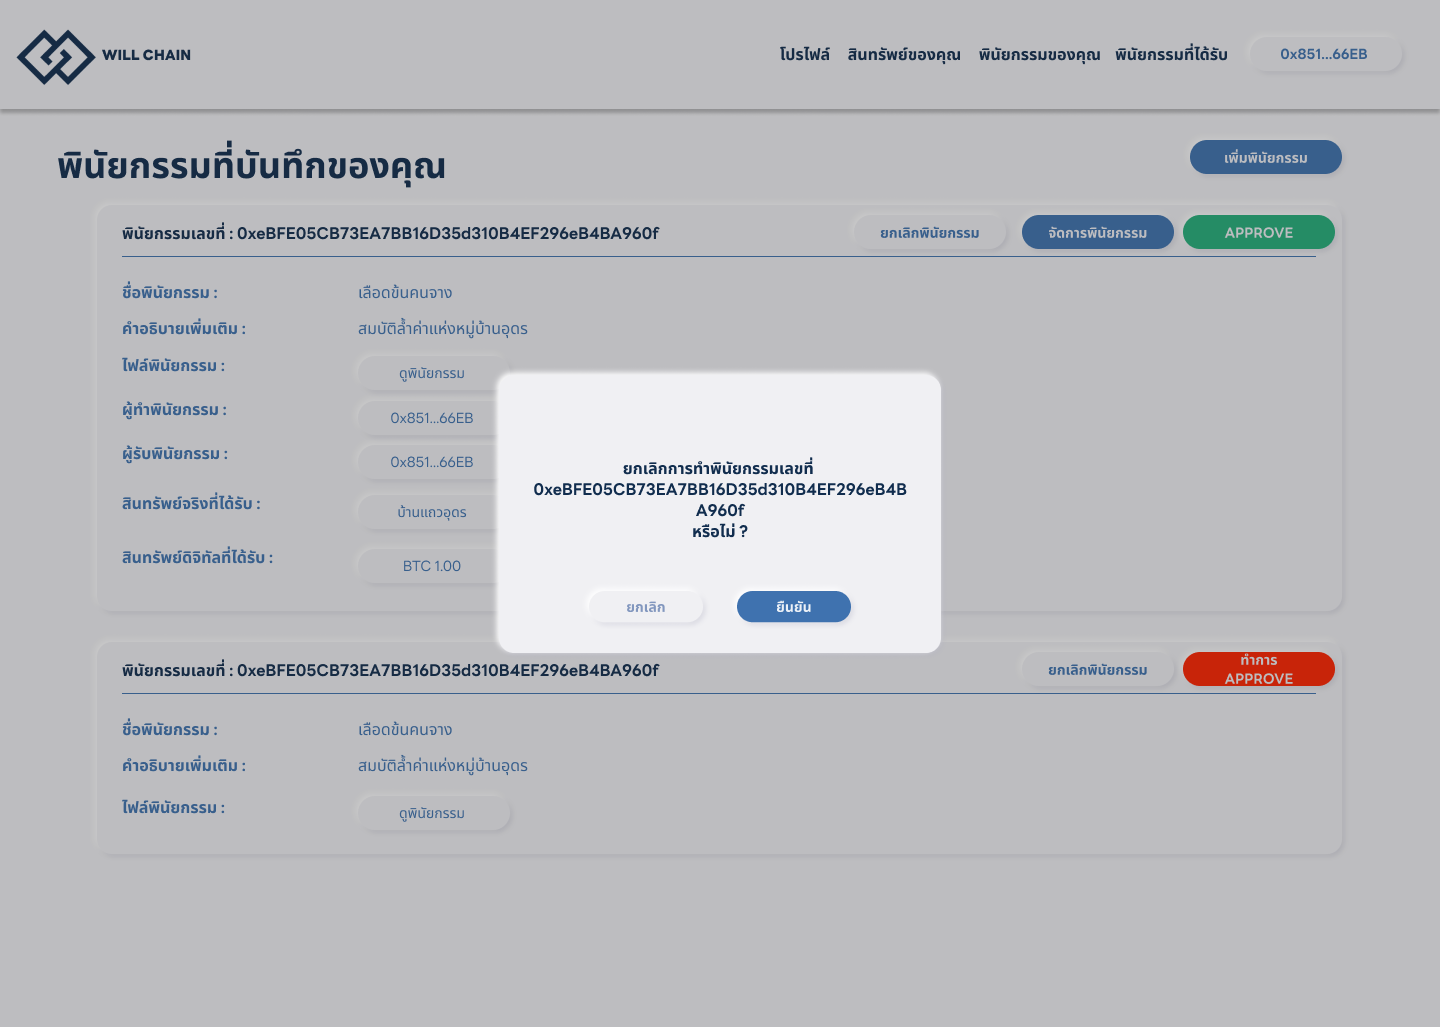
\includegraphics[scale=0.2]{cancelWill}
			\caption{หน้ายกเลิกการทำพินัยกรรมของคุณ}
		\end{figure}
		\FloatBarrier
		\tab จากรูป จะเป็นหน้ายกเลิกการทำพินัยกรรม โดยการกดที่ปุ่ม "ยกเลิกพินัยกรรม" ในหน้าพินัยกรรมของคุณ โดยที่หน้านี้จะแสดงเลขที่ของพินัยกรรม และให้ยืนยันการลบพินัยกรรมฉบับนั้น

\subsection{หน้า Approve พินัยกรรมของคุณ}
		\begin{figure}[!thb]
			\centering
			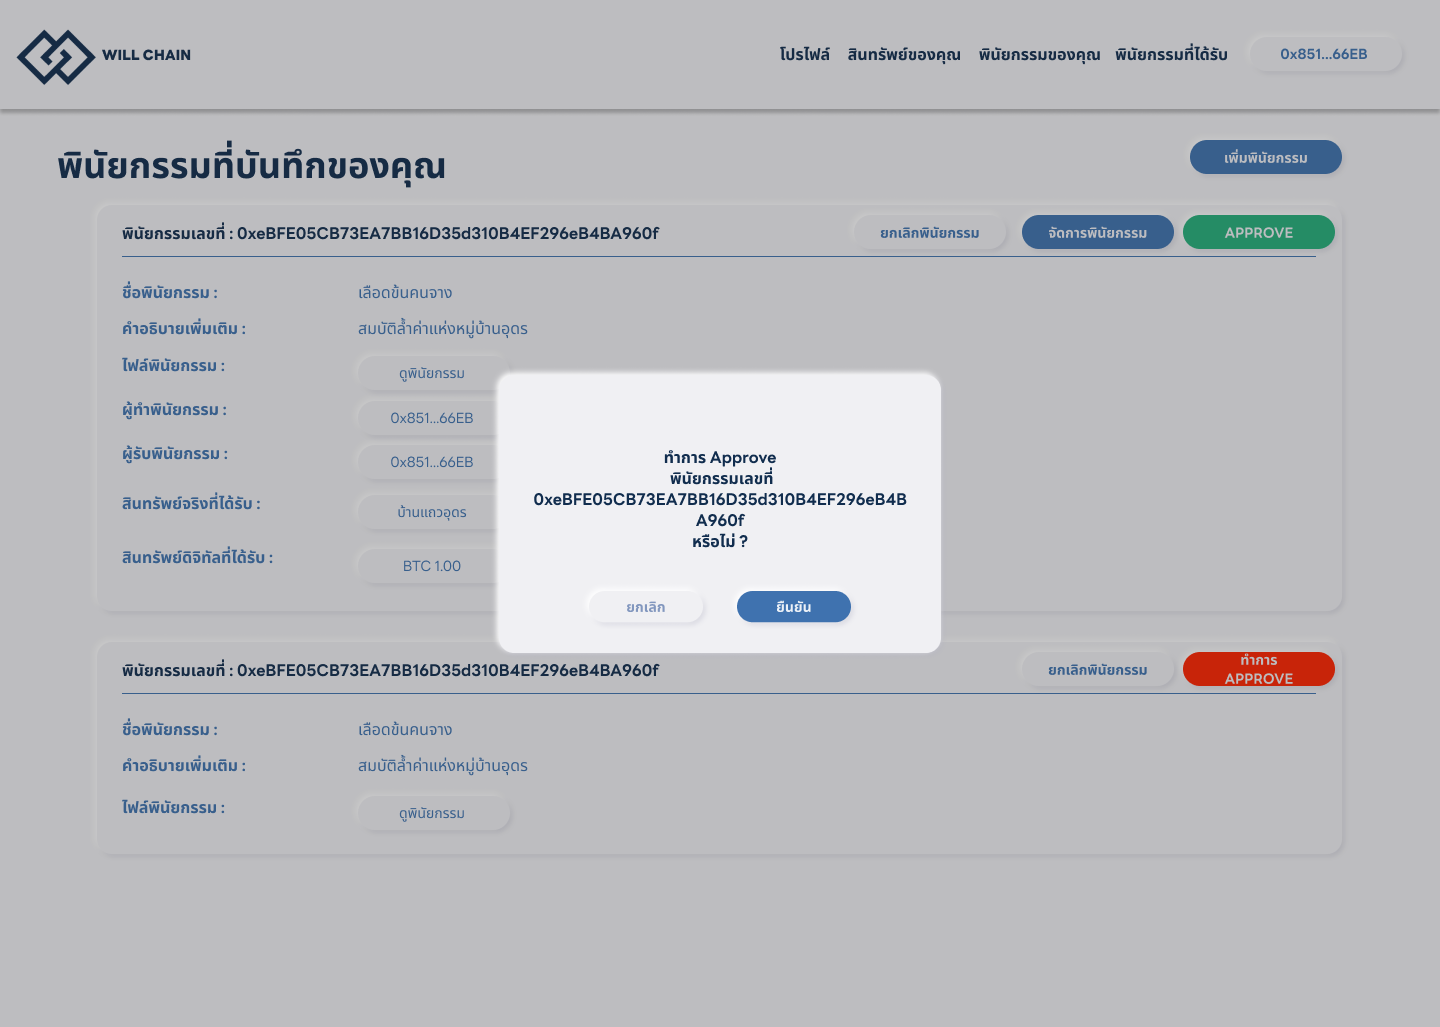
\includegraphics[scale=0.2]{WillApprove}
			\caption{หน้า Approve พินัยกรรมของคุณ}
		\end{figure}
		\FloatBarrier
		\tab จากรูป จะเป็นหน้า Approve พินัยกรรม จากการที่กดปุ่ม "ทำการ Approve" ในหน้าพินัยกรรมของคุณ โดยที่หน้านี้จะแสดงยืนยันการ Approve ของพินัยกรรมให้ระบบของ Will Chain ดูแลเรื่องพินัยกรรมให้
\subsection{หน้าบันทึกพินัยกรรม}
		\begin{figure}[!thb]
			\centering
			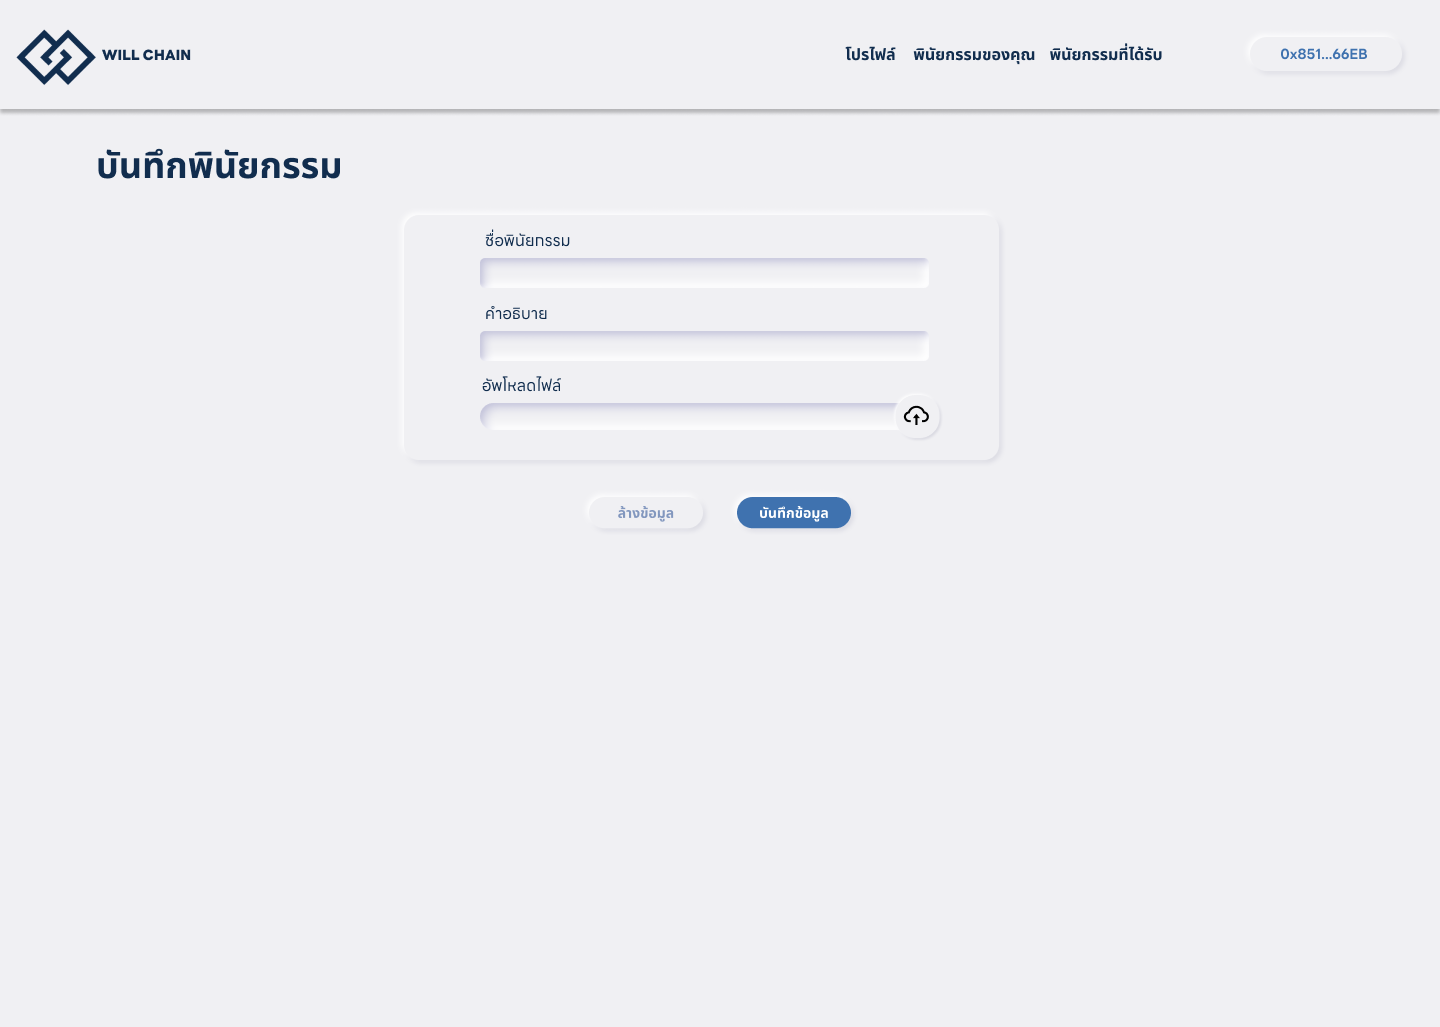
\includegraphics[scale=0.2]{saveWill}
			\caption{หน้าบันทึกพินัยกรรม}
		\end{figure}
		\FloatBarrier
		\tab  จากรูป เป็นหน้าบันทึกพินัยกรรม โดยสามารถบันทึกพินัยกรรมได้ที่หน้านี้ โดยจะเข้าหน้านี้หลังจากกดที่ปุ่ม “เพิ่มพินัยกรรม” ในหน้าพินัยกรรมของคุณ โดยที่จะมีฟอร์มให้ใส่ข้อมูลของพินัยกรรม 3 รายการ ได้แก่ (1) ชื่อพินัยกรรม (2) รายละเอียดของพินัยกรรมฉบับนี้ และ (3) อัพโหลดไฟล์พินัยกรรมฉบับจริง
		
\clearpage
\subsection{หน้าจัดการสินทรัพย์ภายในพินัยกรรมของคุณ}
		\begin{figure}[!thb]
			\centering
			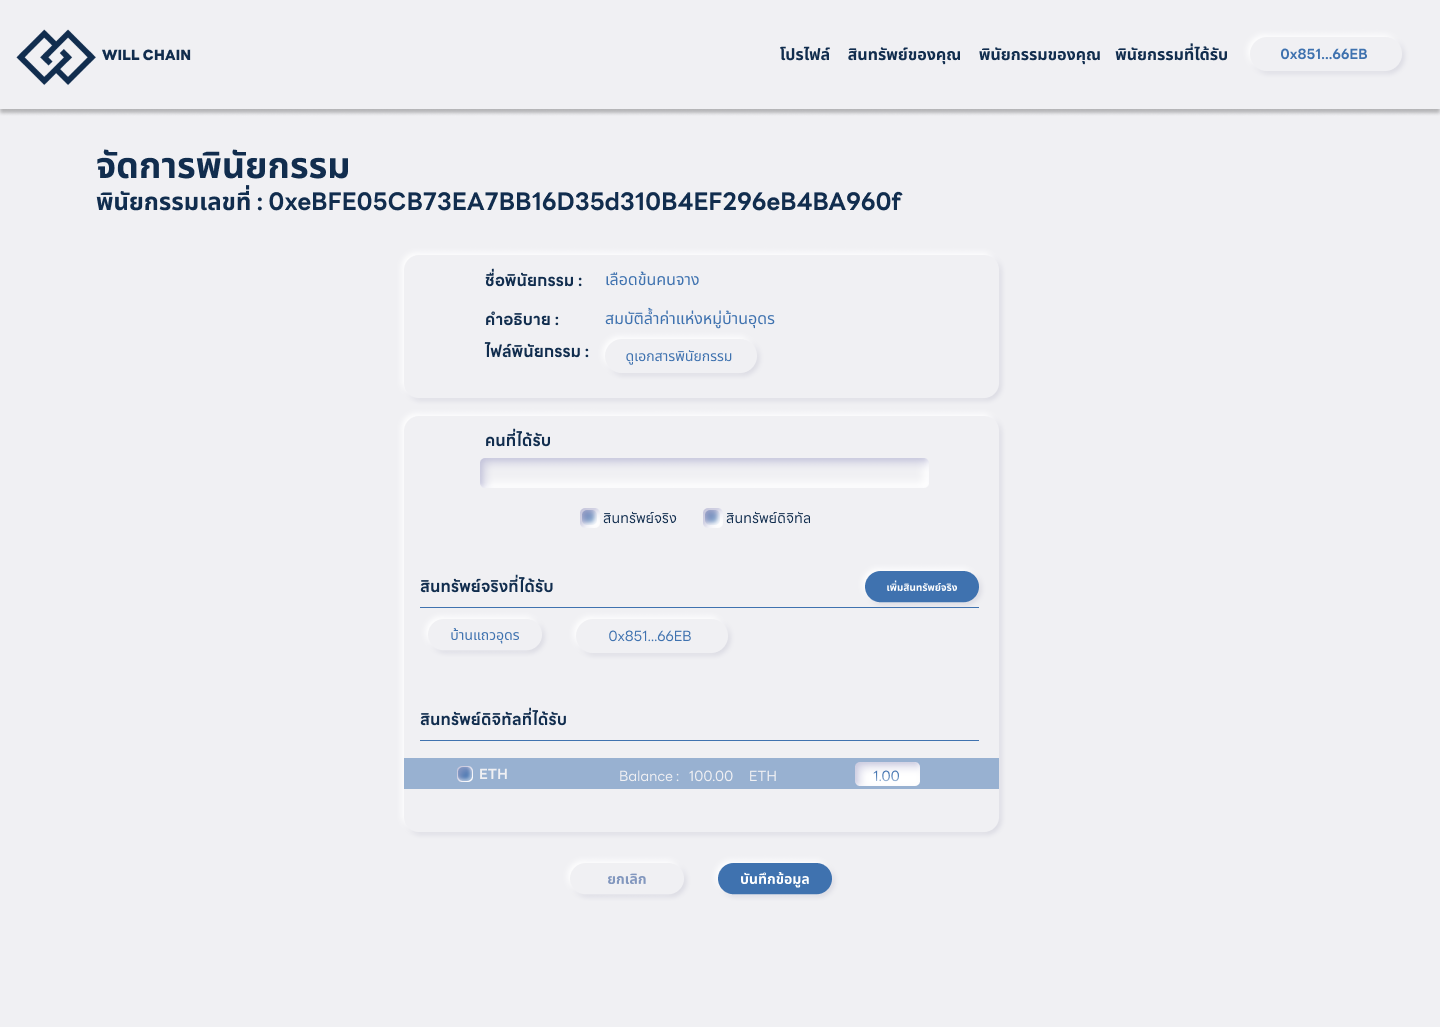
\includegraphics[scale=0.2]{manageWill}
			\caption{หน้าจัดการสินทรัพย์ภายในพินัยกรรมของคุณ}
		\end{figure}
		\FloatBarrier
		\tab  จากรูป จะเป็นหน้าจัดการสินทรัพย์ภายในพินัยกรรมของคุณ จากการที่กดเมนู "จัดการพินัยกรรม" ในหน้าพินัยกรรมของคุณ โดยที่หน้านี้จะแสดงการจัดการพินัยกรรมโดยจะแสดงเลขที่พินัยกรรม , ชื่อพินัยกรรม, รายละเอียดพินัยกรรม และพินัยกรรมฉบับจริงในรูปแบบไฟล์ โดยหน้านี้จะสามารถเพิ่มเติมข้อมูล เช่น การใส่เลขกระเป๋า MetaMask Wallet ของผู้รับพินัยกรรมได้ , สามารถเพิ่มสินทรัพย์จริงเพื่อทำการสร้างเป็น NFT และแสดงรายละเอียดทรัพย์สินได้ และสามารถเพิ่มเหรียญสินทรัพย์ดิจิทัลได้
\subsection{หน้าเพิ่มสินทรัพย์จริง}
		\begin{figure}[!thb]
			\centering
			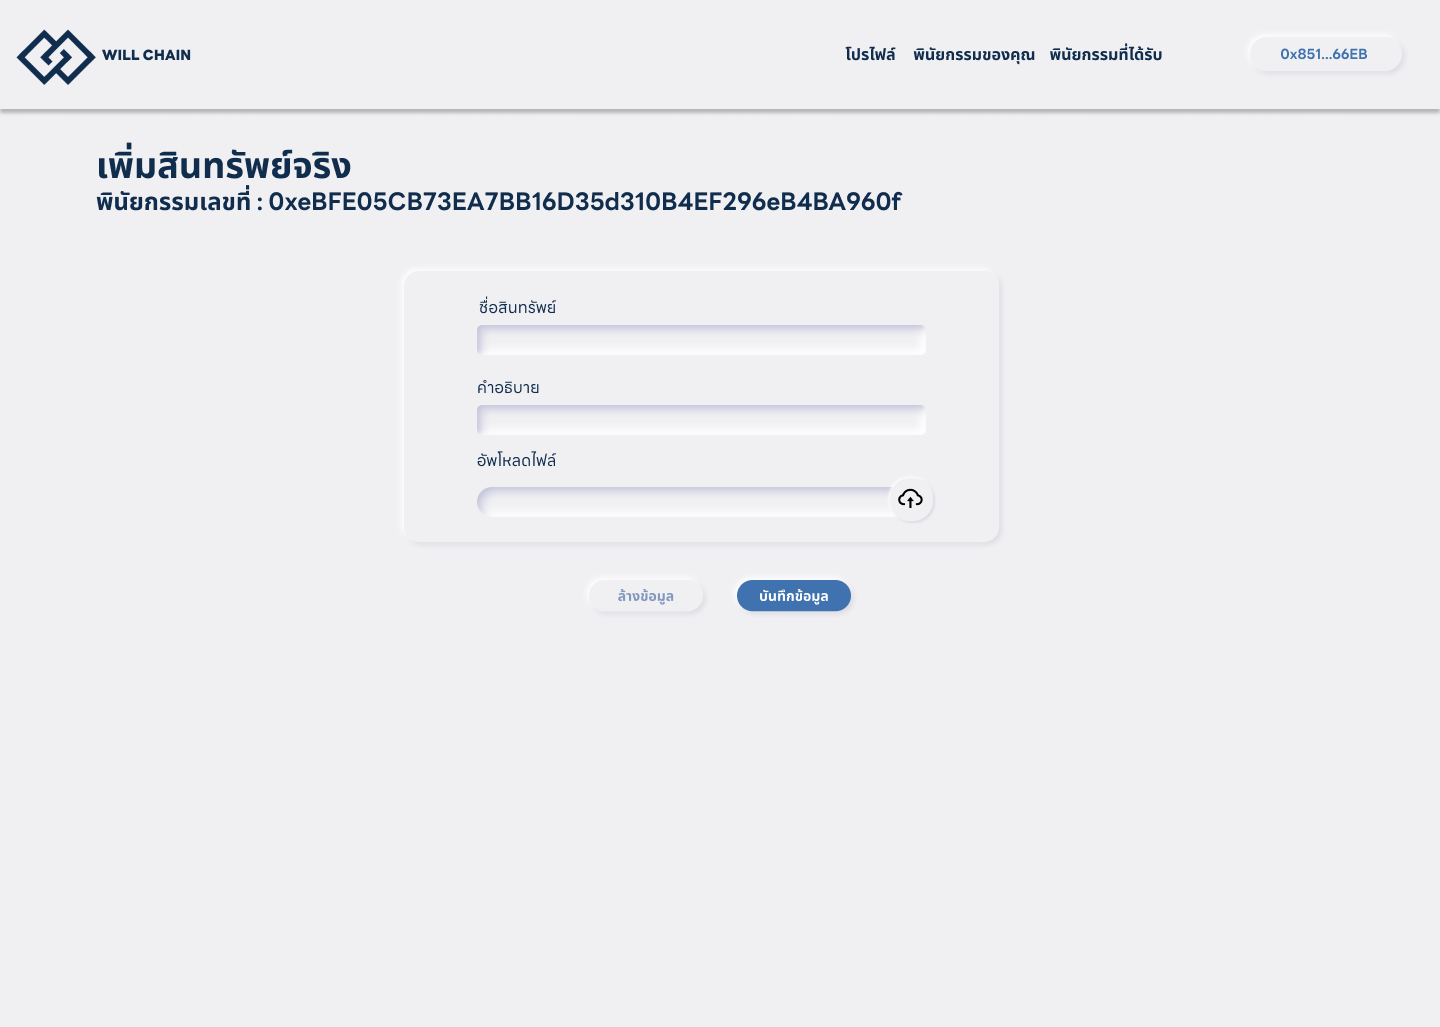
\includegraphics[scale=0.2]{addRealAsset}
			\caption{หน้าเพิ่มสินทรัพย์จริง}
		\end{figure}
		\FloatBarrier
		\tab จากรูป เป็นหน้าเพิ่มสินทรัพย์จริงเข้าสู่พินัยกรรม ที่เมื่อกดที่ปุ่ม "เพิ่มสินทรัพย์จริง" จะเข้าสู่หน้านี้ โดยที่จะแสดงเลขพินัยกรรมที่กำลังจะเพิ่มสินทรัพย์จริง โดยจะมีฟอร์มให้ใส่ข้อมูล 3 รายการ ได้แก่ (1) ชื่อสินทรัพย์จริง (2) คำอธิบายเกี่ยวกับสินทรัพย์จริงนั้น และ (3) ไฟล์สำหรับยืนยันว่าครอบครองพินัยกรรมนั้นจริง ๆ เช่น โฉนดที่ดิน , บ้าน , เล่มทะเบียนรถ เป็นต้น
		
\clearpage
\subsection{หน้าพินัยกรรมที่ได้รับ}
		\begin{figure}[!thb]
			\centering
			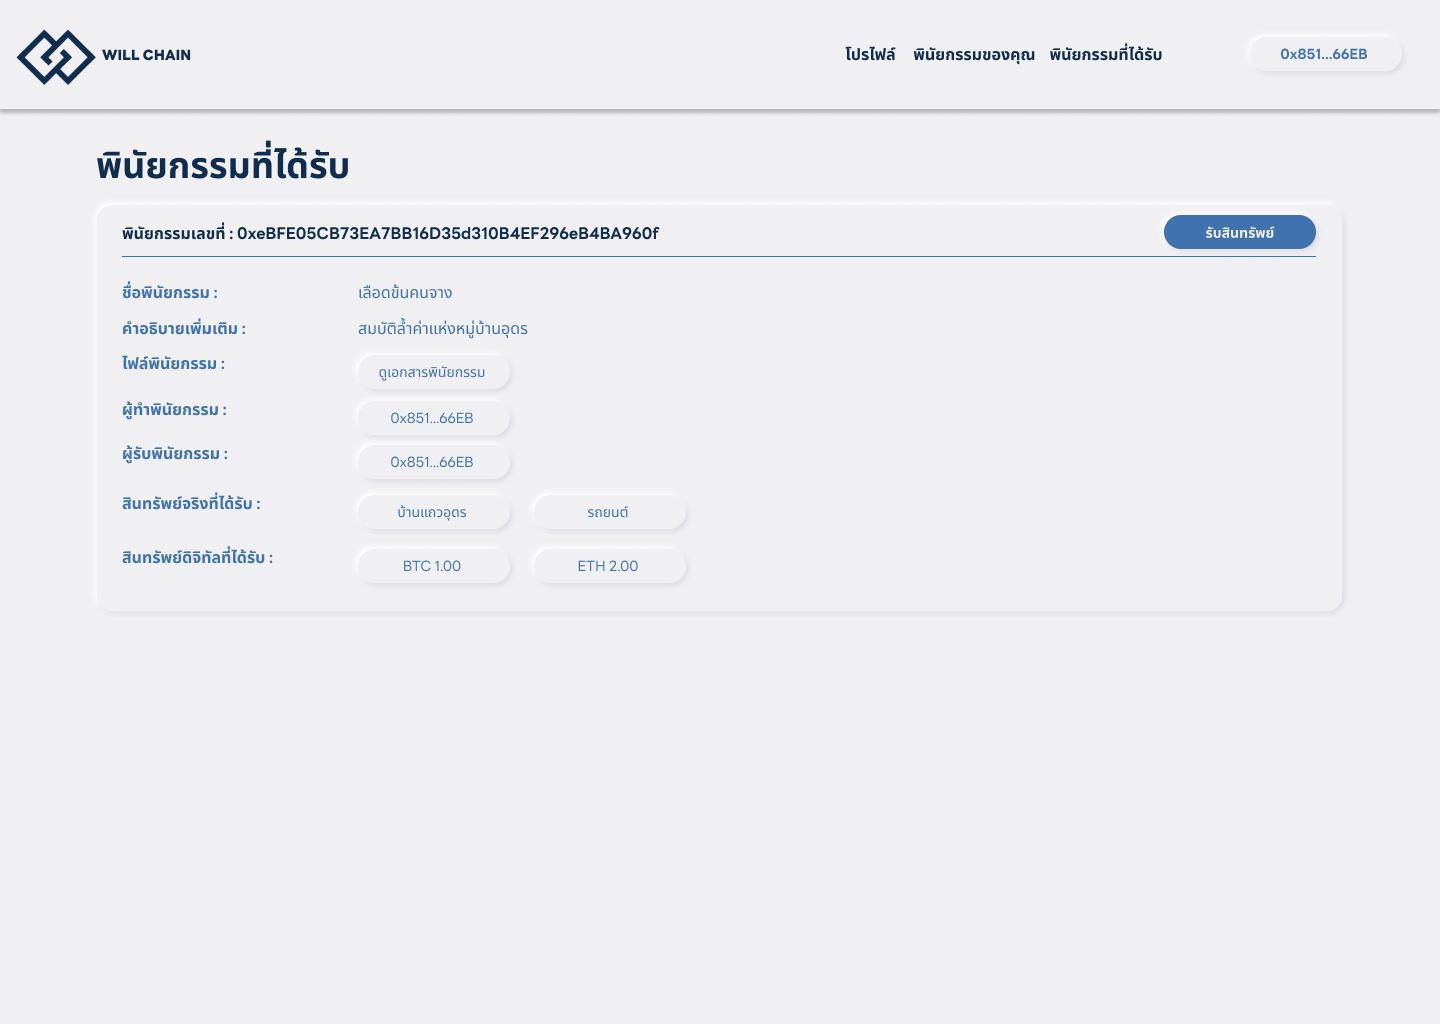
\includegraphics[scale=0.2]{claimWill}
			\caption{พินัยกรรมที่ได้รับ}
		\end{figure}
		\FloatBarrier
		\tab จากรูป เป็นหน้าพินัยกรรมที่ได้รับ ที่หลังจากมีการส่งต่อพินัยกรรมเนื่องมาจากการเสียชีวิต ในหน้านี้จะแสดงพินัยกรรมที่ได้รับ โดยที่สามารถกดปุ่ม “ดูพินัยกรรม” ที่จะสามารถดูพินัยกรรมที่เป็นฉบับจริงได้ และในตารางจะมีแสดงรายละเอียดของคนที่ได้รับ ผู้รับพินัยกรรม ผู้สร้างพินัยกรรม สินทรัพย์จริงที่ได้รับ สินทรัพย์ดิจิทัลที่ได้รับ อีกทั้งสามารถกดรับสินทรัพย์ได้จากปุ่ม "รับสินทรัพย์'' ด้านขวาบน
\subsection{หน้ายืนยันรับพินัยกรรม}
		\begin{figure}[!thb]
			\centering
			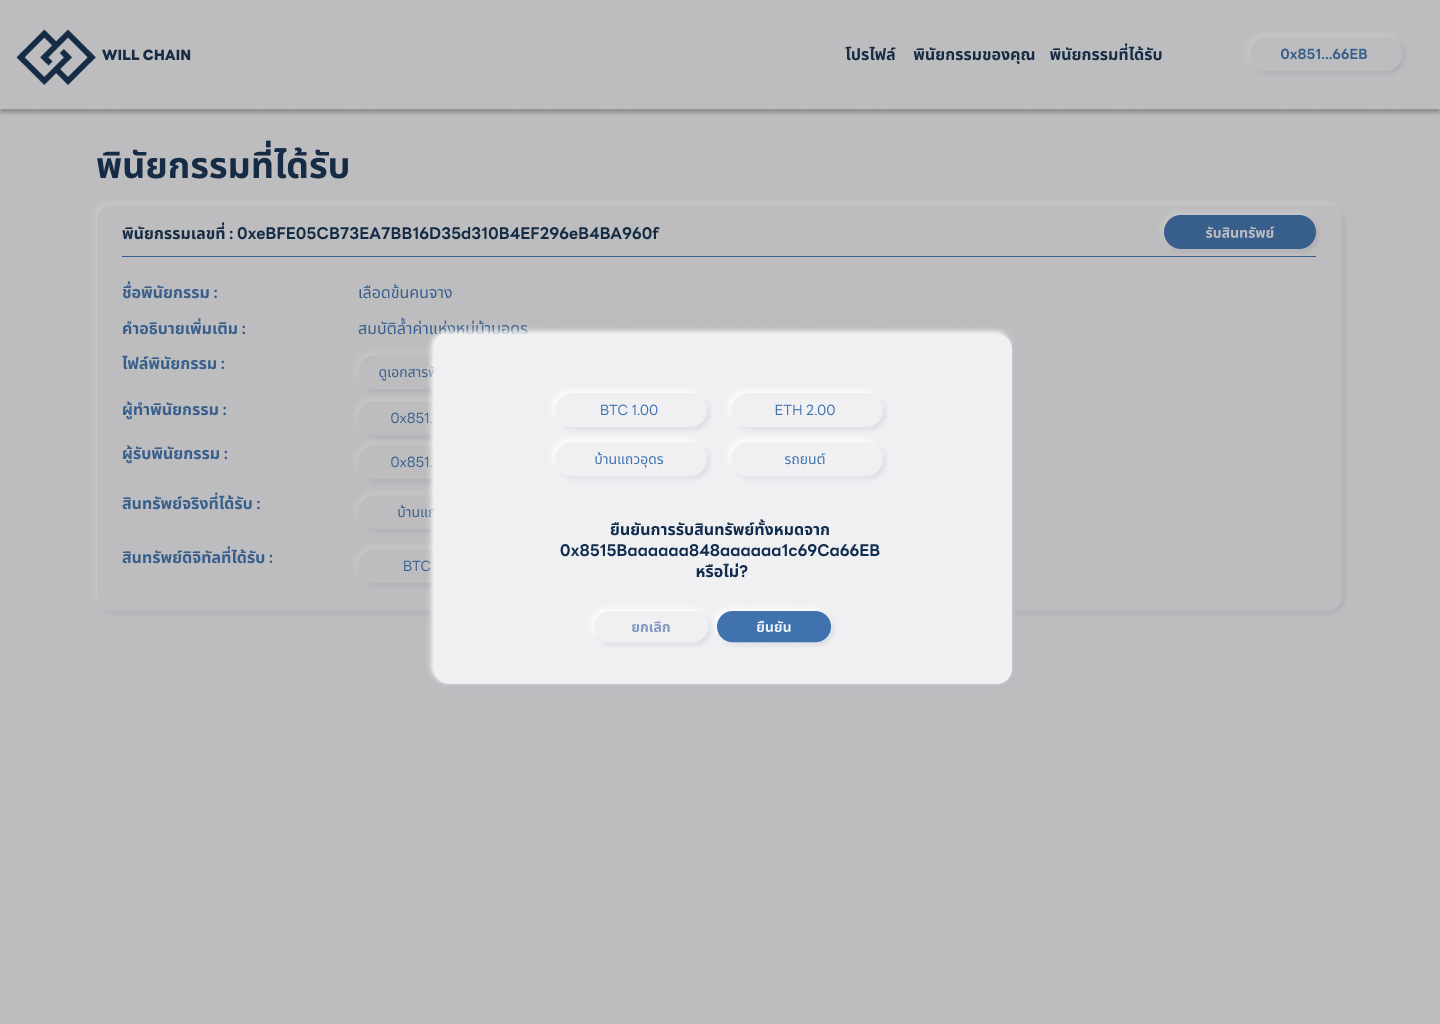
\includegraphics[scale=0.2]{claimWillConfirm}
			\caption{หน้ายืนยันรับพินัยกรรม}
		\end{figure}
		\FloatBarrier
		\tab จากรูป เป็นหน้ายืนยันการรับพินัยกรรมโดยจะทำการเลือกสินทรัพย์ที่ได้รับในแต่ละสินทรัพย์ที่อยู่ในพินัยกรรม
		
\clearpage
\subsection{หน้ารับพินัยกรรมเสร็จสิ้น}
		\begin{figure}[!thb]
			\centering
			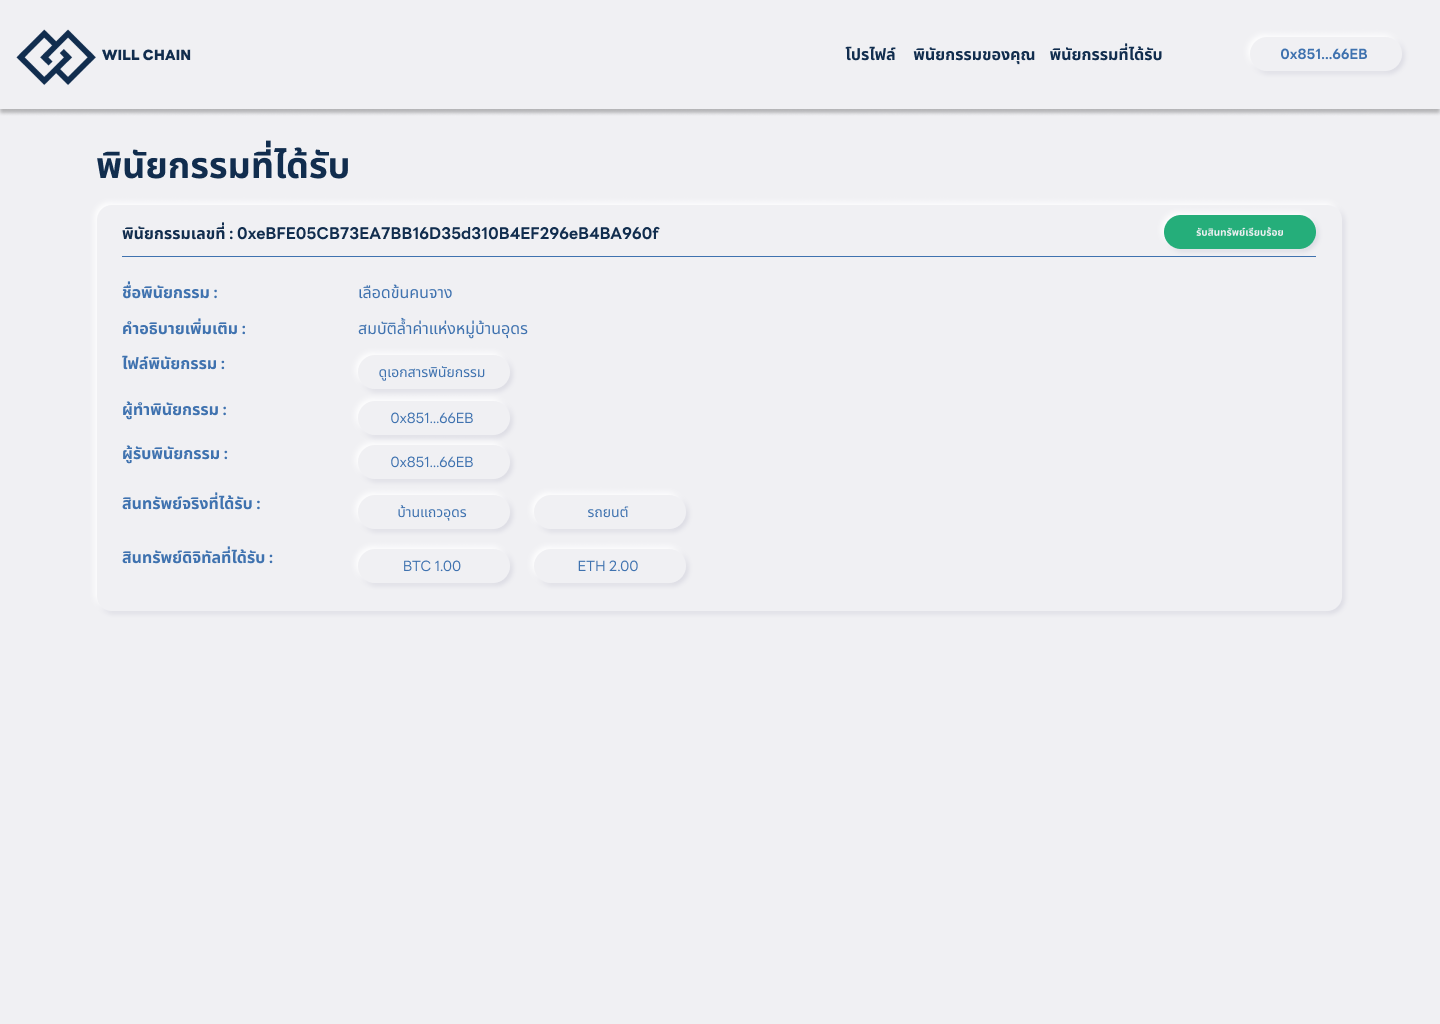
\includegraphics[scale=0.2]{claimWillSuccess}
			\caption{หน้ารับพินัยกรรมเสร็จสิ้น}
		\end{figure}
		\FloatBarrier
		\tab จากรูป เป็นหน้ารับพินัยกรรมเสร็จสิ้น โดยจะเป็นหน้าที่รับสินทรัพย์และรับพินัยกรรมเสร็จสิ้น
\section{ออกแบบการทดสอบ}
\tab ทดสอบด้วยการจำลองการใช้งานผ่าน platform โดยมี function ที่จะทดสอบดั้งนี้
	\begin{enumerate}[label=\thesection.\arabic*,leftmargin=0pt,itemindent=1.25cm]
		\item Function connect MetaMask wallet สําหรับการเชื่อมต่อ Crypto Wallet ของผู้ใช้งานเข้ากับ MetaMask เพื่อเตรียมพร้อมต่อการทดสอบ function อื่น ๆ
		\item Function เกี่ยวกับการจัดการพินัยกรรมรวมถึงการเพิ่มผู้รับผลประโยชน์และสินทรัพย์ 
		\item Function เกี่ยวกับการจัดการสิยทรัพย์ที่ผู้ใช้ทำการลงทะเบียนไว้ในระบบ
		\item Function การส่งพินัยกรรมและสินทรัพย์ไปให้ผู้รับมรดก
	\end{enumerate}

\chapter{ผลการดําเนินงาน}
\section{Site map}
	\subsection{ หน้าหลัก}
	\subsection{หน้าโปรไฟล์}
	\begin{itemize}[leftmargin=0pt,itemindent=1.25cm]
		\item[-] ลงทะเบียนด้วยรหัสเลขบัตรประชาชน
	\end{itemize}
	\subsection{ หน้าพินัยกรรมที่บันทึกของคุณ}
	\begin{itemize}[leftmargin=0pt,itemindent=1.25cm]
		\item[-] ทำการ Approve พินัยกรรมของคุณ
		\item[-] ยกเลิกการทำพินัยกรรม
	\end{itemize}
	\subsection{ หน้าบันทึกพินัยกรรม} 
	\begin{itemize}[leftmargin=0pt,itemindent=1.25cm]
		\item[-] อัพโหลดพินัยกรรม
	\end{itemize}
	\subsection{หน้าจัดการพินัยกรรม}
	\begin{itemize}[leftmargin=0pt,itemindent=1.25cm]
		\item[-] เพิ่มสินทรัพย์จริง
		\item[-] เพิ่มสินทรัพย์ดิจิทัล
		\item[-] เพิ่มผู้รับพินัยกรรม
	\end{itemize}
	\subsection{พินัยกรรมที่ได้รับของคุณ}
	\begin{itemize}[leftmargin=0pt,itemindent=1.25cm]
		\item[-] รับสินทรัพย์
	\end{itemize}

\section{Token ที่ใช้ใน Will-Chain}
\subsection{Any Token Support ERC20}
		\tab Any Token Support ERC20 คือเหรียญที่ใช้มาตรฐาน ERC-20 ที่ซึ่งใช้เพื่อสำหรับฝากเหรียญดิจิทัลเข้าสู่ระบบ Will Chain
		
\subsection{Will Token}
		\tab  Will Token คือ NFT ที่ทำหน้าที่แทนพินัยกรรมซึ่งทำงานบนระบบ Ethereum โดยใช้มาตรฐาน ERC-721 ซึ่ง Will Token จะเป็นตัวที่ต้องใช้ในการที่เราจะสร้างรับสินทรัพย์ที่มีอยู่ในพินัยกรรมของ Will Contract

\subsection{ETH}
		\tab  ETH คือ เหรียญดิจิทัลที่ใช้เทคโนโลยีบล็อกเชนทำงานอยู่เบื้องหลัง เพื่อใช้จ่ายสำหรับค่าธรรมเนียม สำหรับทุก Smart Contract ที่ผู้ใช้งานต้องการจะใช้บน Ethereum chain
\clearpage
\subsection{Real Token}	
		\tab Real Token คือ NFT ที่ทำหน้าที่แทนสินทรัพย์จริงซึ่งทำงานบนระบบ Ethereum โดยใช้มาตรฐาน ERC-721 
\section{Test Plan}

\subsection {Validation Testing }
	\begin{itemize}
		\item ตรวจสอบว่า Software ตรงตาม Requirement หรือไม่
		\item บันทึกข้อผิดพลาดพร้อมกับการแก้ไข
	\end{itemize}
\subsection {Verification Testing }
	\begin{itemize}
		\item  ตรวจสอบว่า Software ออกแบบได้ตรงตาม UX/UI ที่ออกแบบไว้หรือไม่
		\item ตรวจสอบว่า Software ออกแบบได้ตรงตาม Architecture หรือไม่
		\item ตรวจสอบว่า Software ออกแบบได้ตรงตาม UML design หรือไม่
	\end{itemize}
\clearpage

\section{Web Application Will Chain}
\subsection{Home Page}
	\begin{figure}[!thb]
			\centering
			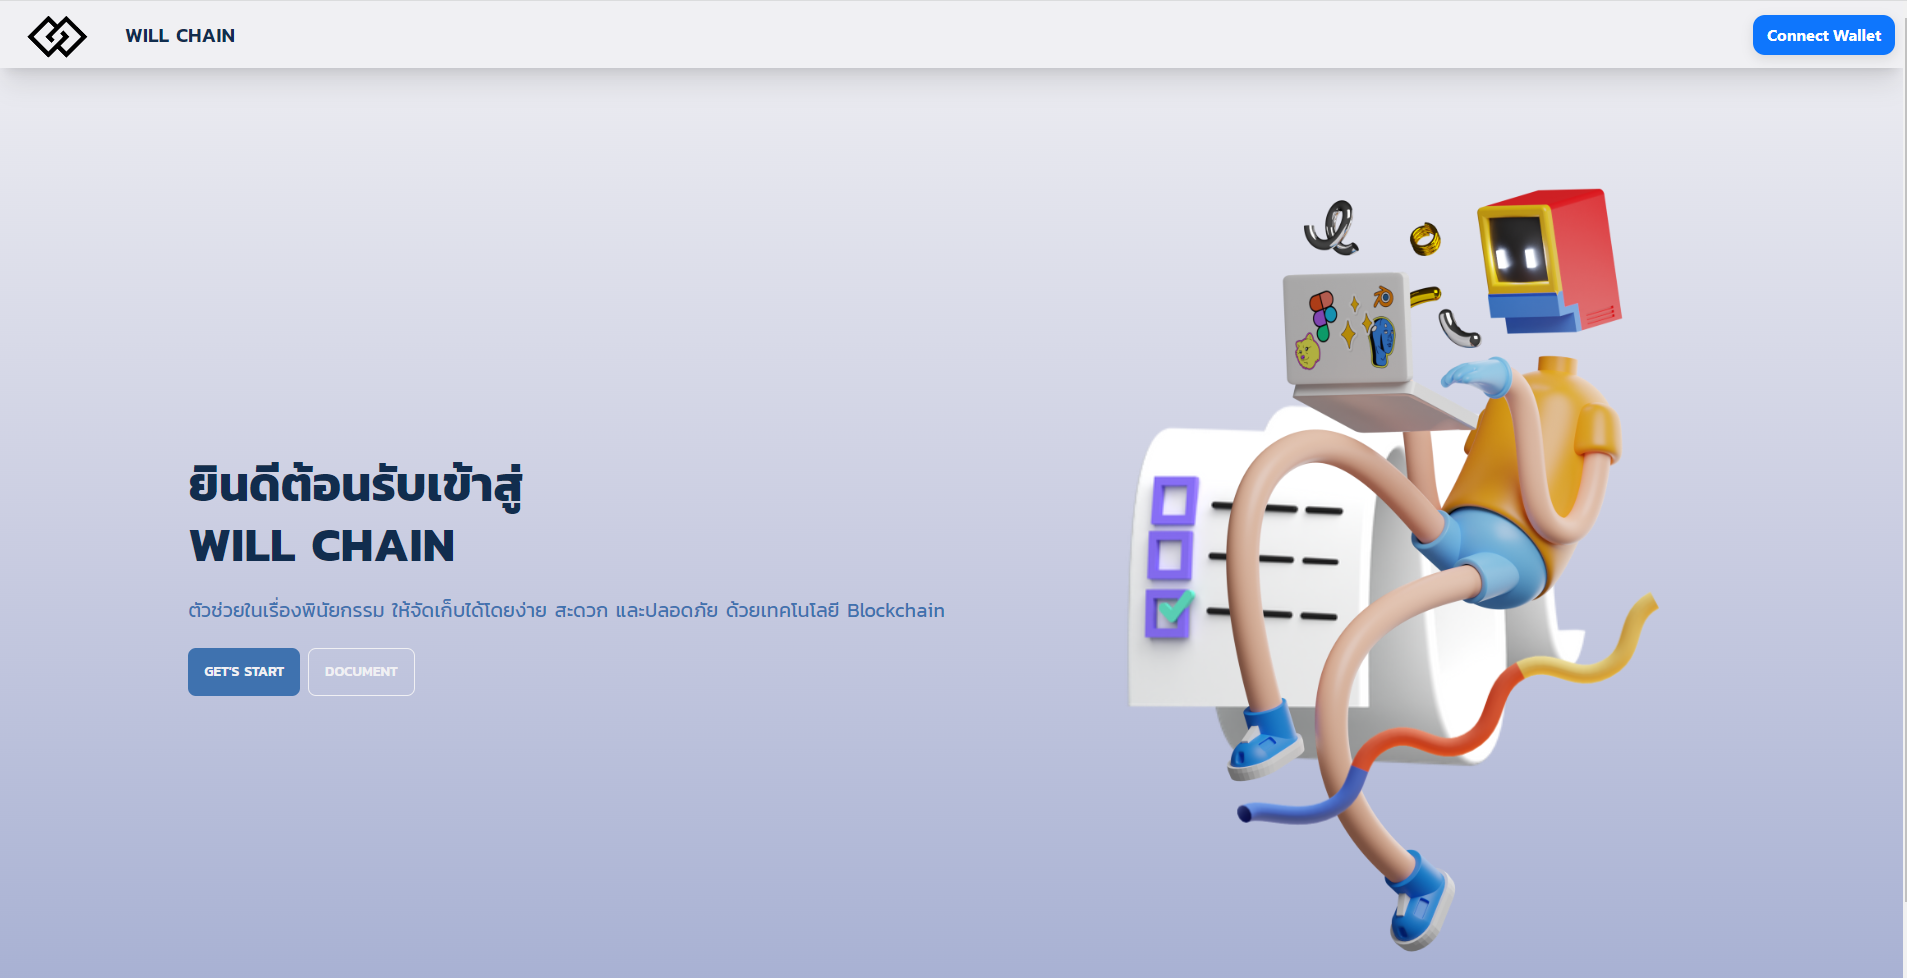
\includegraphics[scale=0.2]{homePageBefore4}
			\caption{Home Page}
		\end{figure}
		\FloatBarrier
\tab เป็นหน้าแรกของแพลตฟอร์ม Will Chain โดยเมื่อผู้ใช้งานเข้ามาจะเห็นปุ่ม Connect wallet ที่ให้ผู้ใช้ สามารถเลือกการเข้าสู่ระบบด้วย Crypto Wallet ที่ต้องการ 
\subsection{Select Login Provider Wallet}
	\begin{figure}[!thb]
			\centering
			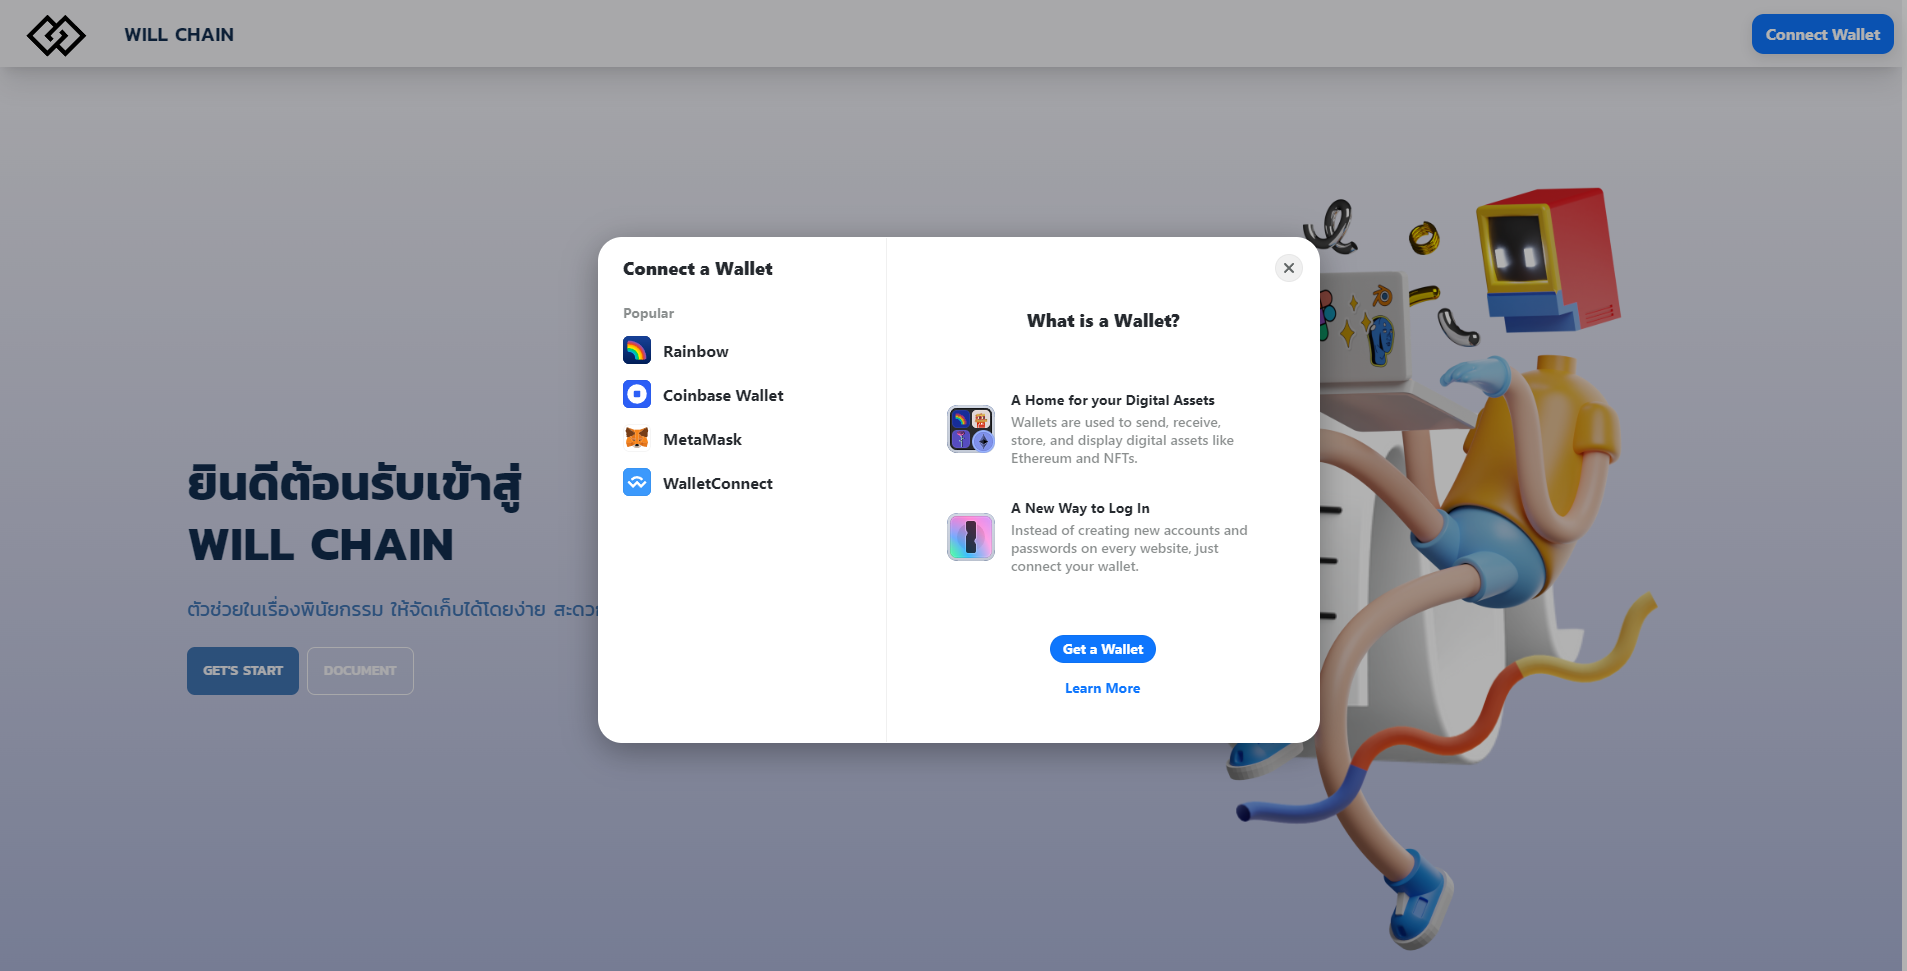
\includegraphics[scale=0.2]{homePageSelect4}
			\caption{Select Login Provider Wallet}
		\end{figure}
		\FloatBarrier
\tab เมื่อผู้ใช้ทำการคลิกที่ปุ่ม Connect wallet จะปรากฎหน้าเมนูขึ้นมาให้ผู้ใช้เลือกชนิดของ Crypto Wallet ที่จะทำการเชื่อมเข้าสู่ระบบ หากผู้ใช้ไม่มี Crypto Wallet จะมีปุ่มให้ผู้ใช้ทำการสมัคร Crypto Wallet ก่อนพร้อมทั้งบอกข้อมูลเบื้องต้นของ Crypto Wallet นั้น ๆ 

\clearpage

\subsection{Login By Metamask Wallet}
	\begin{figure}[!thb]
			\centering
			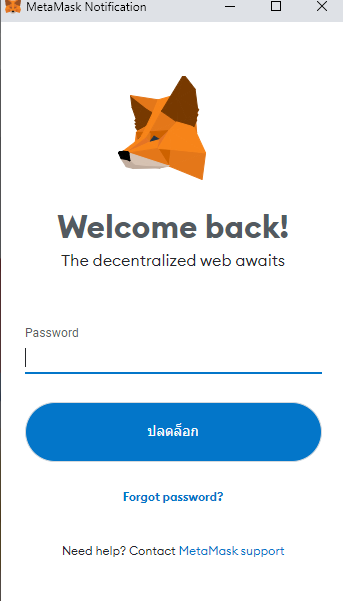
\includegraphics[scale=0.5]{metamaskLogin4}
			\caption{Login By MetaMask Wallet}
		\end{figure}
		\FloatBarrier
\tab เมื่อผู้ใช้เลือก Crypto Wallet ที่ต้องการได้แล้ว จะมีหน้าต่างสำหรับการใส่รหัสผ่านเพื่อทำการเข้าสู่ระบบโดยในที่นี้เลือกเป็น MetaMask Wallet 
\subsection{Home Page Logged in}
	\begin{figure}[!thb]
			\centering
			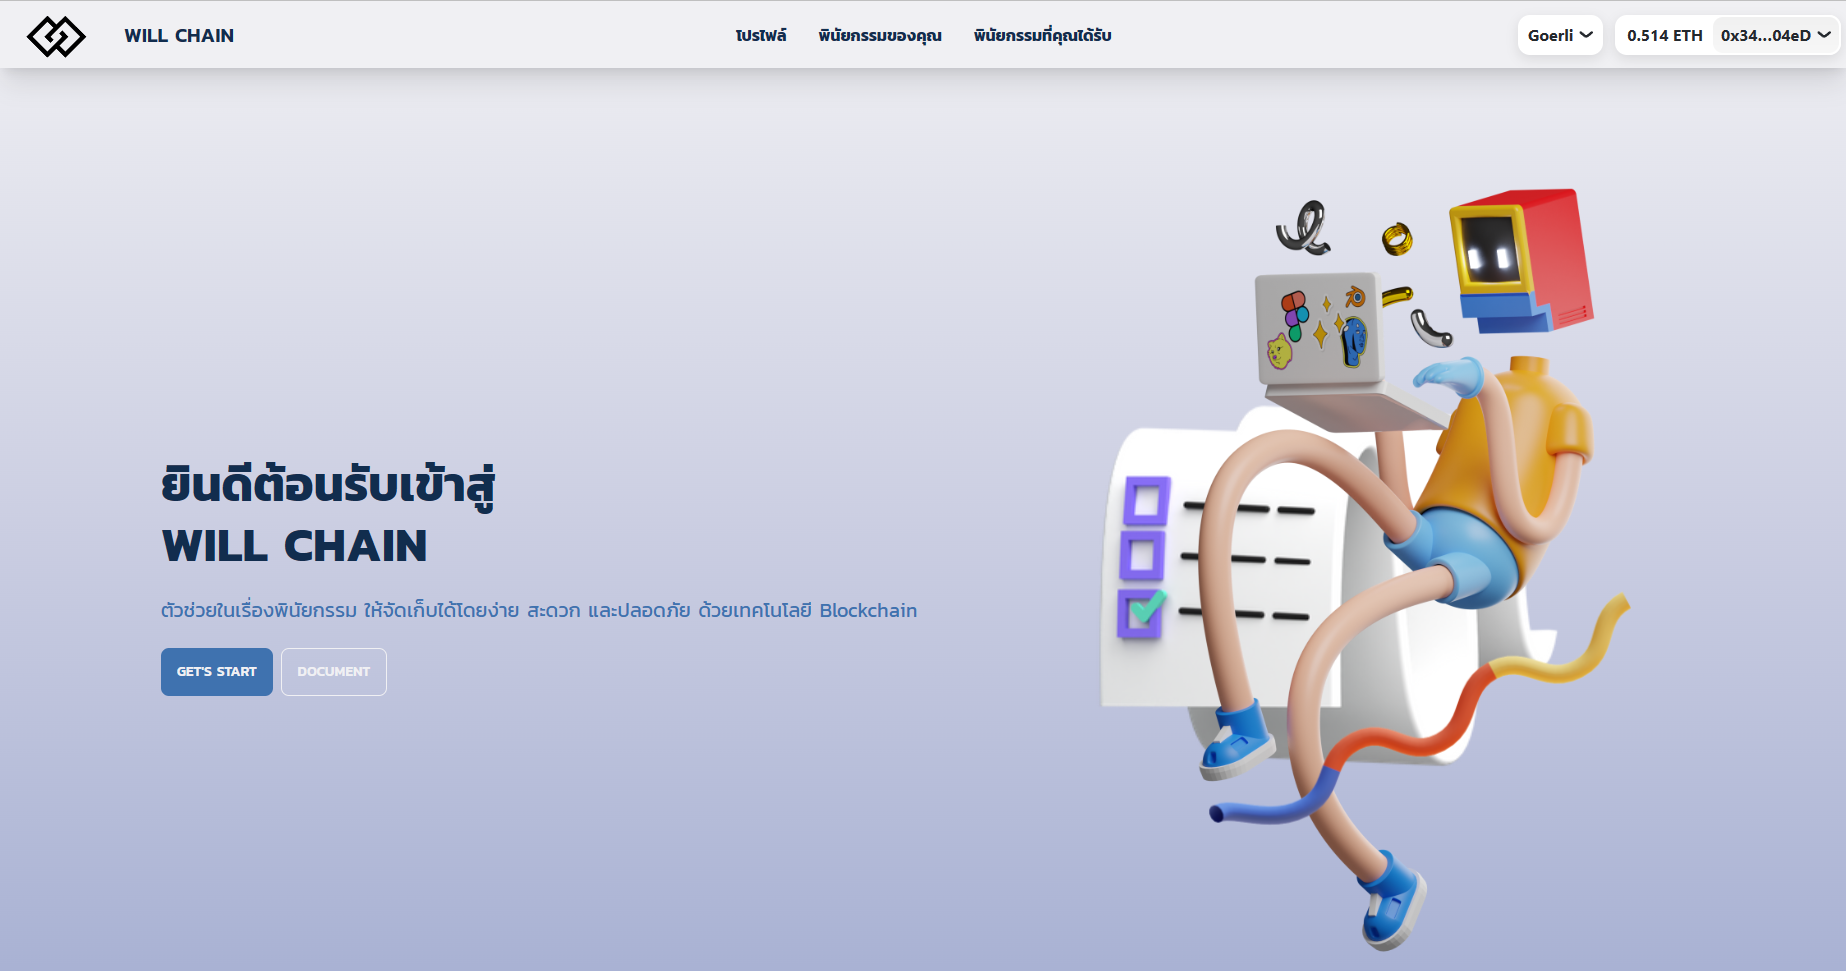
\includegraphics[scale=0.2]{homePageAfter4}
			\caption{Home Page Logged in }
		\end{figure}
		\FloatBarrier
\tab เมื่อผู้ใช้เข้าสู่ระบบแล้วจะมีการเปลี่ยนแถบเมนูที่ด้านบน โดยจะแสดงข้อมูลบัญชีของผู้ใช้ ได้แก่ Chain ที่ใช้งานอยู่ในขณะนั้น จำนวนเงินคงเหลือ และเลข address ของบัญชี CryptoWallet นั้น ๆ 

\clearpage
\subsection{Profile Page}
	\begin{figure}[!thb]
			\centering
			\includegraphics[scale=0.2]{Profile4}
			\caption{Profile Page}
		\end{figure}
		\FloatBarrier
\tab จากรูป หลังจากกดเมนู ''โปรไฟล์'' ที่แถบเมนูด้านบน จะเข้ามาที่หน้า ''โปรไฟล์'' เพื่อให้ผู้ใช้งานทำการยืนยันเลขบัตรประชาชนเพื่อเข้าใช้งานฟีเจอร์ต่าง ๆ ในระบบ ได้แก่ เมนู ''พินัยกรรมของคุณ'' และ ''พินัยกรรมที่คุณได้รับ''
\subsection{Your Will Page }
	\begin{figure}[!thb]
			\centering
			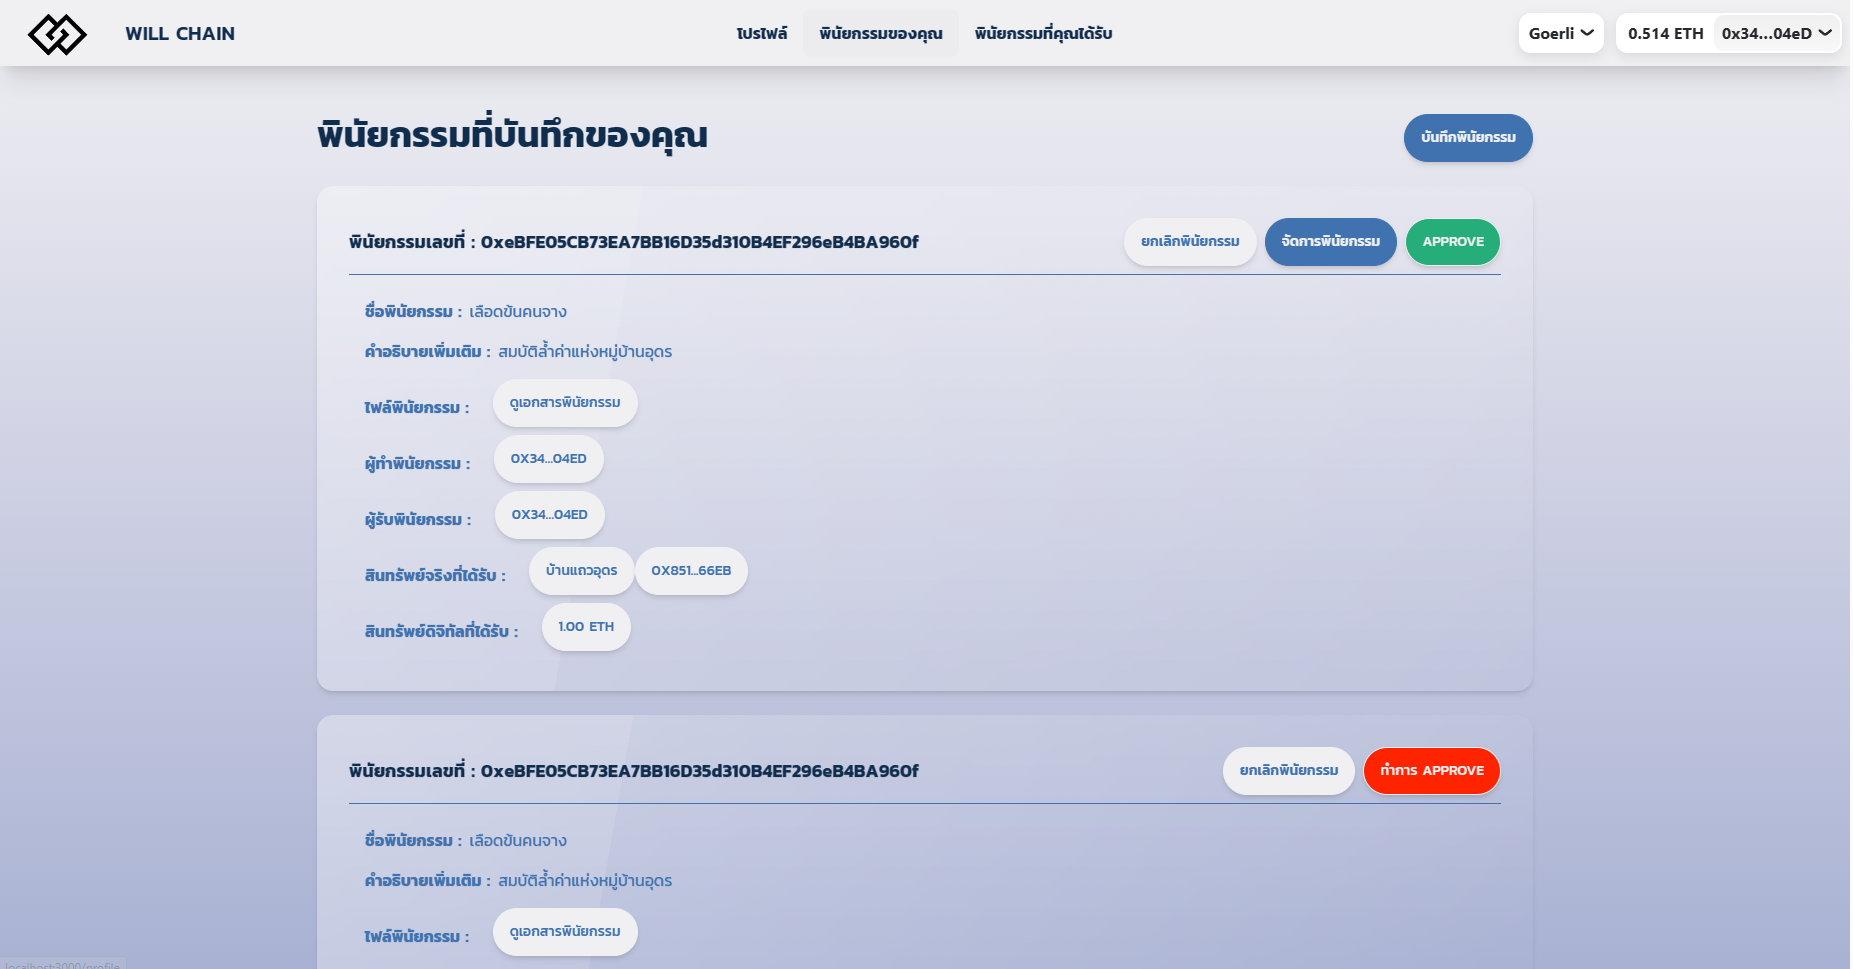
\includegraphics[scale=0.2]{myWill4}
			\caption{My Will Page}
		\end{figure}
		\FloatBarrier
\tab จากรูป หลังจากกดที่เมนู ''พินัยกรรมของคุณ'' ที่แถบเมนูด้านบน จะทำการแสดงหน้าพินัยกรรมที่บันทึกของคุณ โดยในหน้านี้จะแสดงพินัยกรรมที่ผู้ใช้เคยสร้างไว้ และสามารถกดปุ่ม ''บันทึกพินัยกรรม'' เพื่อไปสู่หน้าสำหรับการบันทึกพินัยกรรม ในส่วนของ
พินัยกรรมที่เคยสร้างที่ได้แสดงไว้นั้นจะแสดงข้อมูล เลขที่ของพินัยกรรม ชื่อพินัยกรรม คำอธิบาย ผู้ทำพินัยกรรม ผู้รับพินัยกรรม สินทรัพย์จริงที่ได้รับ สินทรัพย์ดิจิทัลที่ได้รับ โดยสามารถกดที่ปุ่ม ''ยกเลิกพินัยกรรม'' เพื่อยกเลิกการทำพินัยกรรมฉบับนั้น ต่อมาคือปุ่ม ''จัดการพินัยกรรม'' ที่จะสามารถแก้ไขในส่วนของพินัยกรรมและสินทรัพย์ของพินัยกรรมนั้น ๆ ได้ โดยก่อนจะทำการจัดการพินัยกรรม ต้องทำการ Approve พินัยกรรมฉบับนั้น ๆ เสียก่อน ซึ่งถ้าผ่านการ Approve แล้วจะขึ้นแสดงสถานะเป็นปุุ่มสีเขียว แต่ถ้ายังไม่ได้ทำการ Approve จะแสดงเป็นปุ่มสีแดงให้ทำการกดเพื่อ Approve ก่อนที่จะสามรถจัดการพินัยกรรมฉบับนั้น ๆ  ได้

\clearpage
\subsection{Create Will Page }
	\begin{figure}[!thb]
			\centering
			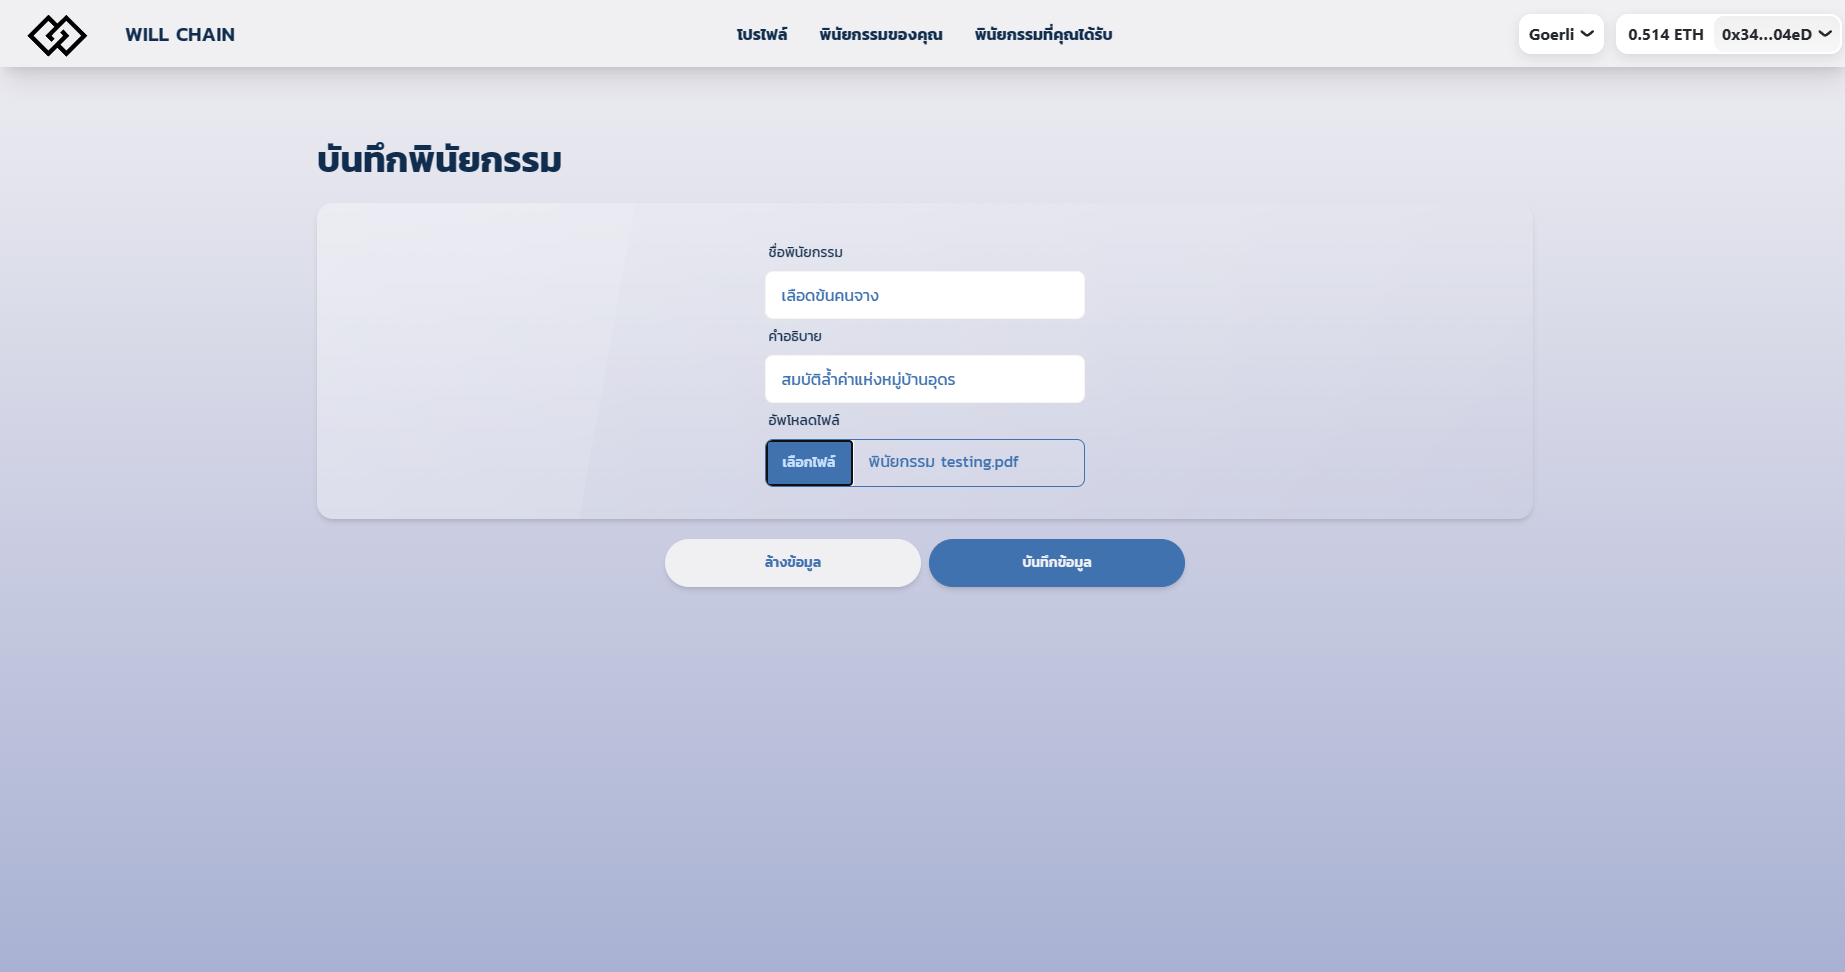
\includegraphics[scale=0.2]{mintWill4}
			\caption{Create Will Page}
		\end{figure}
		\FloatBarrier
\tab จากรูป หลังกดปุ่ม ''บันทึกพินัยกรรม'' ระบบจะนำผู้ใช้งานเข้าสู่หน้าบันทึกพินัยกรรม เพื่อให้ผู้ใช้งานทำการกรอกข้อมูลของพินัยกรรมรวมทั้ง upload file พินัยกรรมเข้าสู่ระบบ โดยที่จะมีปุ่มล้างข้อมูลเพื่อลบข้อมูลทั้งหมดออกและมีปุ่ม บันทึกข้อมูลเพื่อบันทึกพินัยกรรมเข้าสู่ระบบ

\subsection{Manage Will Page}
	\begin{figure}[!thb]
			\centering
			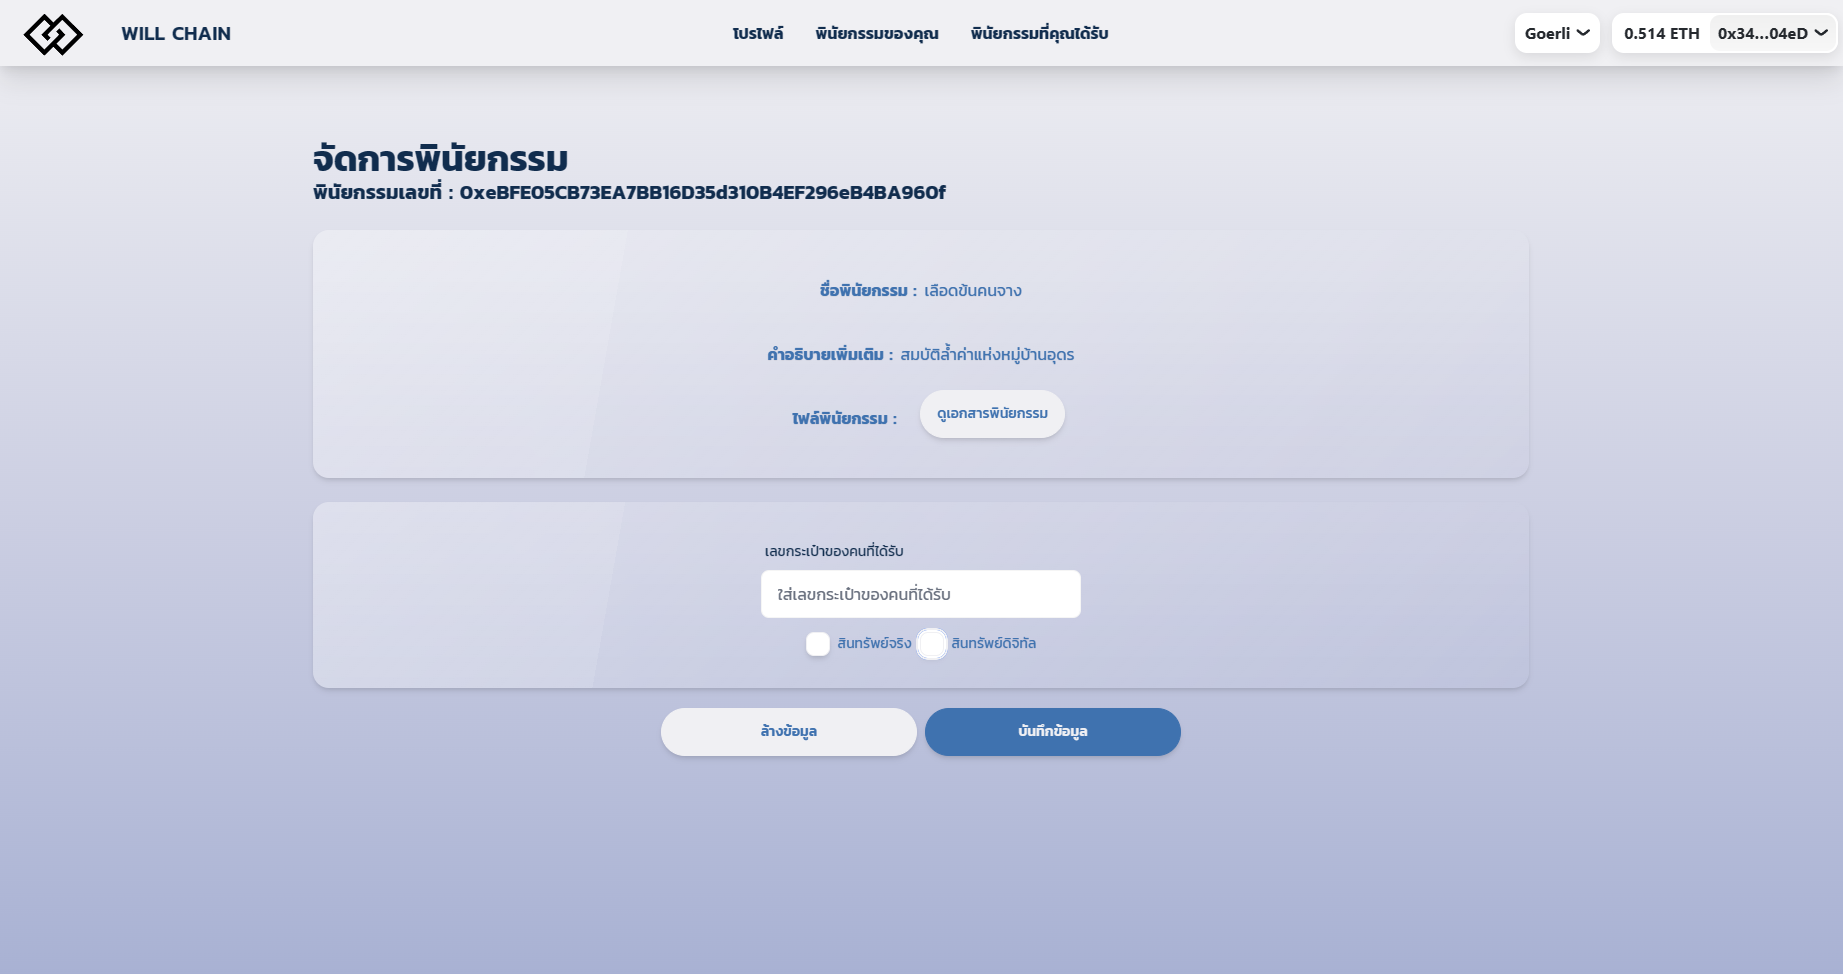
\includegraphics[scale=0.2]{manageWill4}
			\caption{Manage Will Page}
		\end{figure}
		\FloatBarrier
\tab จากรูป หลังจากกดปุ่ม ''จัดการพินัยกรรม'' จะมีฟอร์มให้ใส่ address wallet ของผู้รับพินัยกรรม และ เมนูที่ให้เลือกชนิดของสินทรัพยืที่ต้องการแนบไปในพินัยกรรม โดยแบ่งเป็น สินทรัพย์จริงและสินทรัพย์ดิจิทัล 

\clearpage
\subsection{Add Real Assets }
	\begin{figure}[!thb]
			\centering
			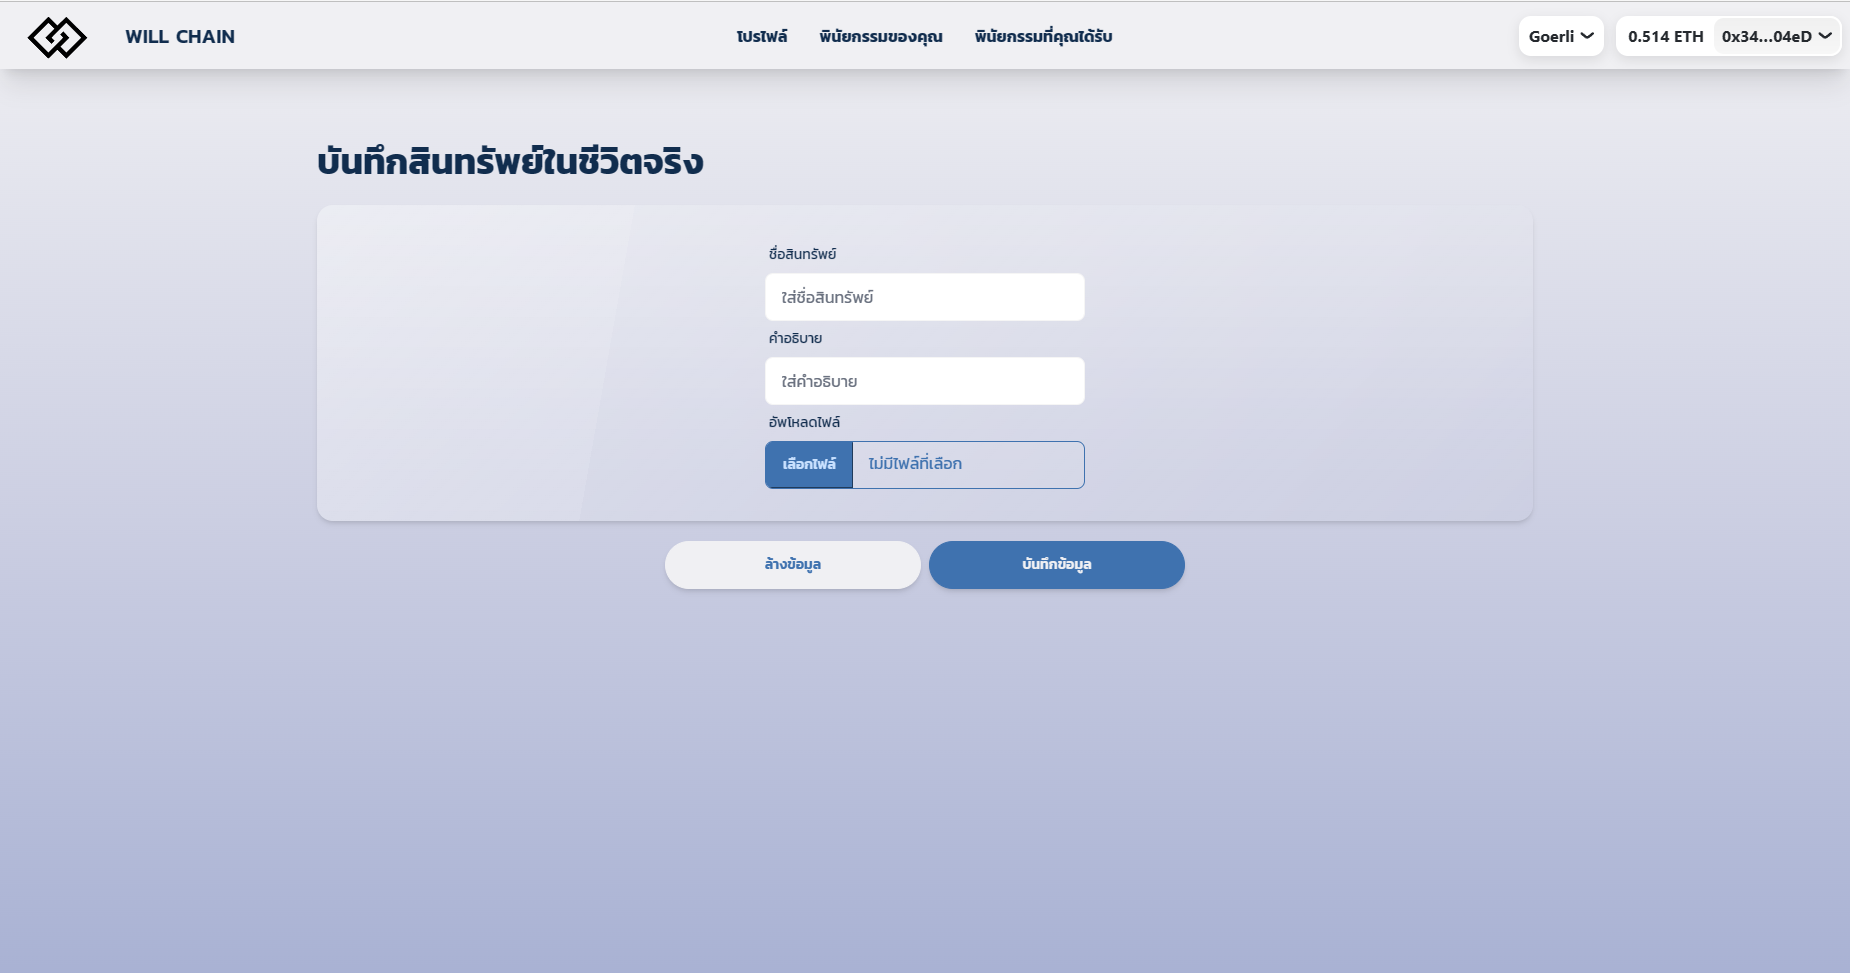
\includegraphics[scale=0.2]{Addwillpage}
			\caption{Add Real Asset page}
		\end{figure}
		\FloatBarrier
\tab จากรูป หลังจากกดปุ่ม ''เพิ่มสินทรัพย์จริง'' ระบบจะทำการเข้าสู่หน้าที่ให้ผู้ใช้กรอกรายละเอียดสินทรัพย์จริงพร้อมทั้งหลักฐานการครอบครองสินทรัพย์ และมีปุ่มล้างข้อมูลเพื่อลบข้อมูลทั้งหมดออกและปุ่มบันทึกข้อมูลเพื่อบันทึกสินทรัพย์

\subsection{Manage Will Page }
	\begin{figure}[!thb]
			\centering
			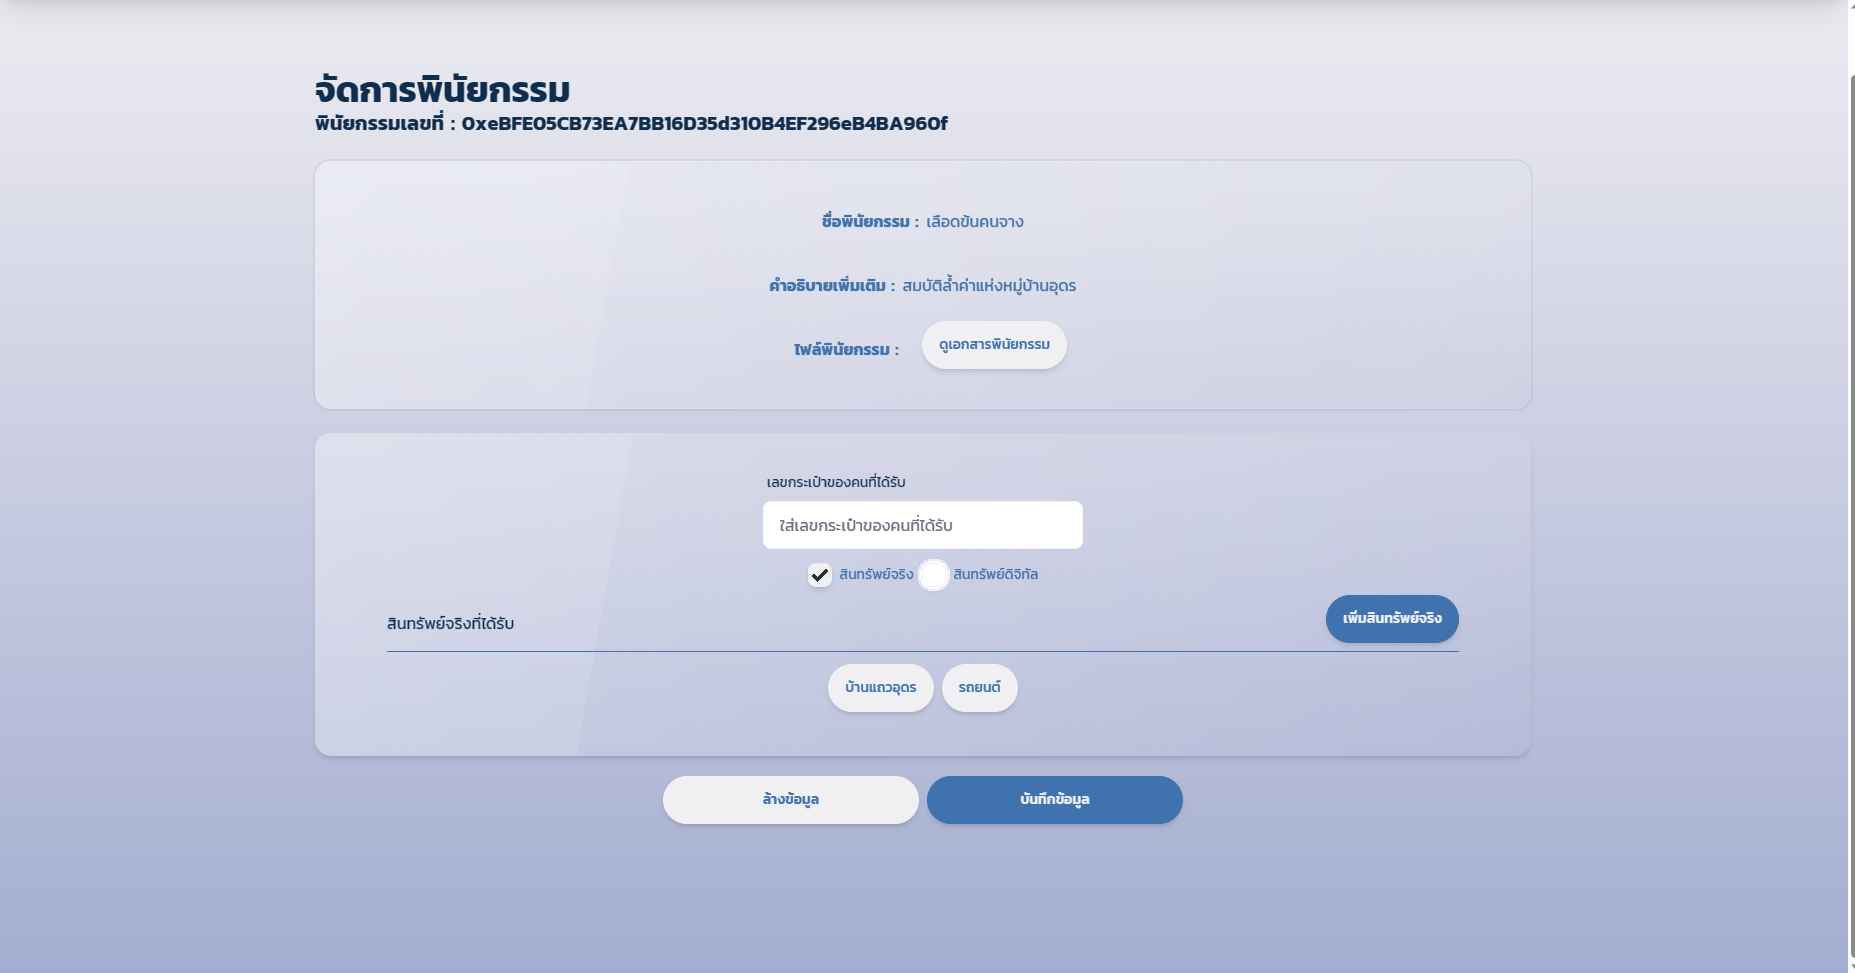
\includegraphics[scale=0.2]{manageWillRealAsset4}
			\caption{Manage Will Page after Add Real Assets }
		\end{figure}
		\FloatBarrier
\tab จากรูป หลังจากกดที่ช่อง ''สินทรัพย์จริง'' จะทำการแสดง component ของสินทรัพย์จริงที่ได้รับ โดยถ้ามีสินทรัพย์จริงอยู่แล้ว จะแสดงสินทรัพย์นั้น ๆ และมีปุ่ม ''เพิ่มสินทรัพย์จริง'' เพื่อทำการเพิ่มสินทรัพย์จริงในหน้าต่อไป
ทำการเพิ่มสินทรัพย์ดิจิทัลระบบจะทำการแสดงสินทรัพยดิจิทัลขึ้นที่หน้าจอพร้อมบอกจำนวนที่ทำการใส่ข้อมูลเข้าไป

\clearpage
\subsection{Manage Will Page}
	\begin{figure}[!thb]
			\centering
			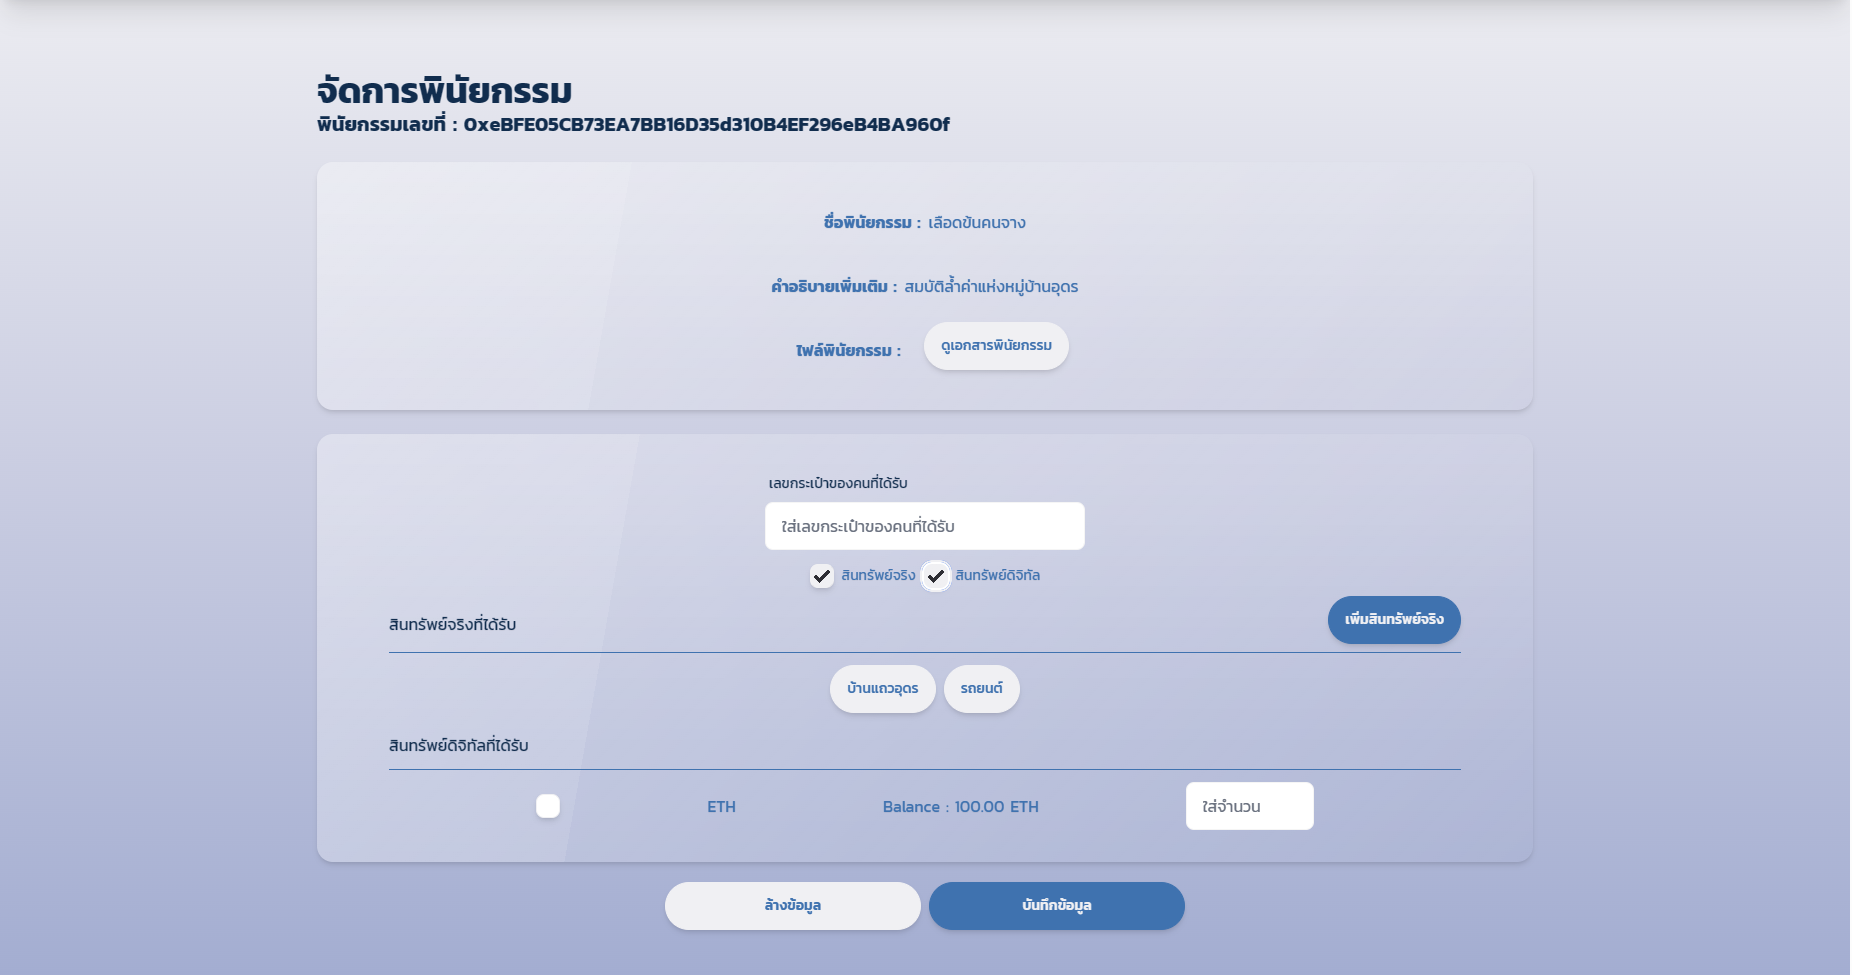
\includegraphics[scale=0.2]{manageWillFullAsset4}
			\caption{Manage Will Page After Add Digital Assets }
		\end{figure}
		\FloatBarrier
\tab จากรูป หลังจากกดที่ช่องที่ช่อง ''สินทรัพย์ดิจิทัล'' จะทำการแสดง component ของสินทรัพย์ดิจิทัล โดยจะทำการเพิ่มสินทรัพย์ดิจิทัลลงในพินัยกรรมนี้ โดยจะทำการแสดงสินทรัพย์ดิจิทัลที่คงเหลือใน MetaMask Wallet และสามารถกรอกจำนวนที่จะใส่เข้าไปในพินัยกรรมได้

\subsection{Beneficiary Claim Will Page }
	\begin{figure}[!thb]
			\centering
			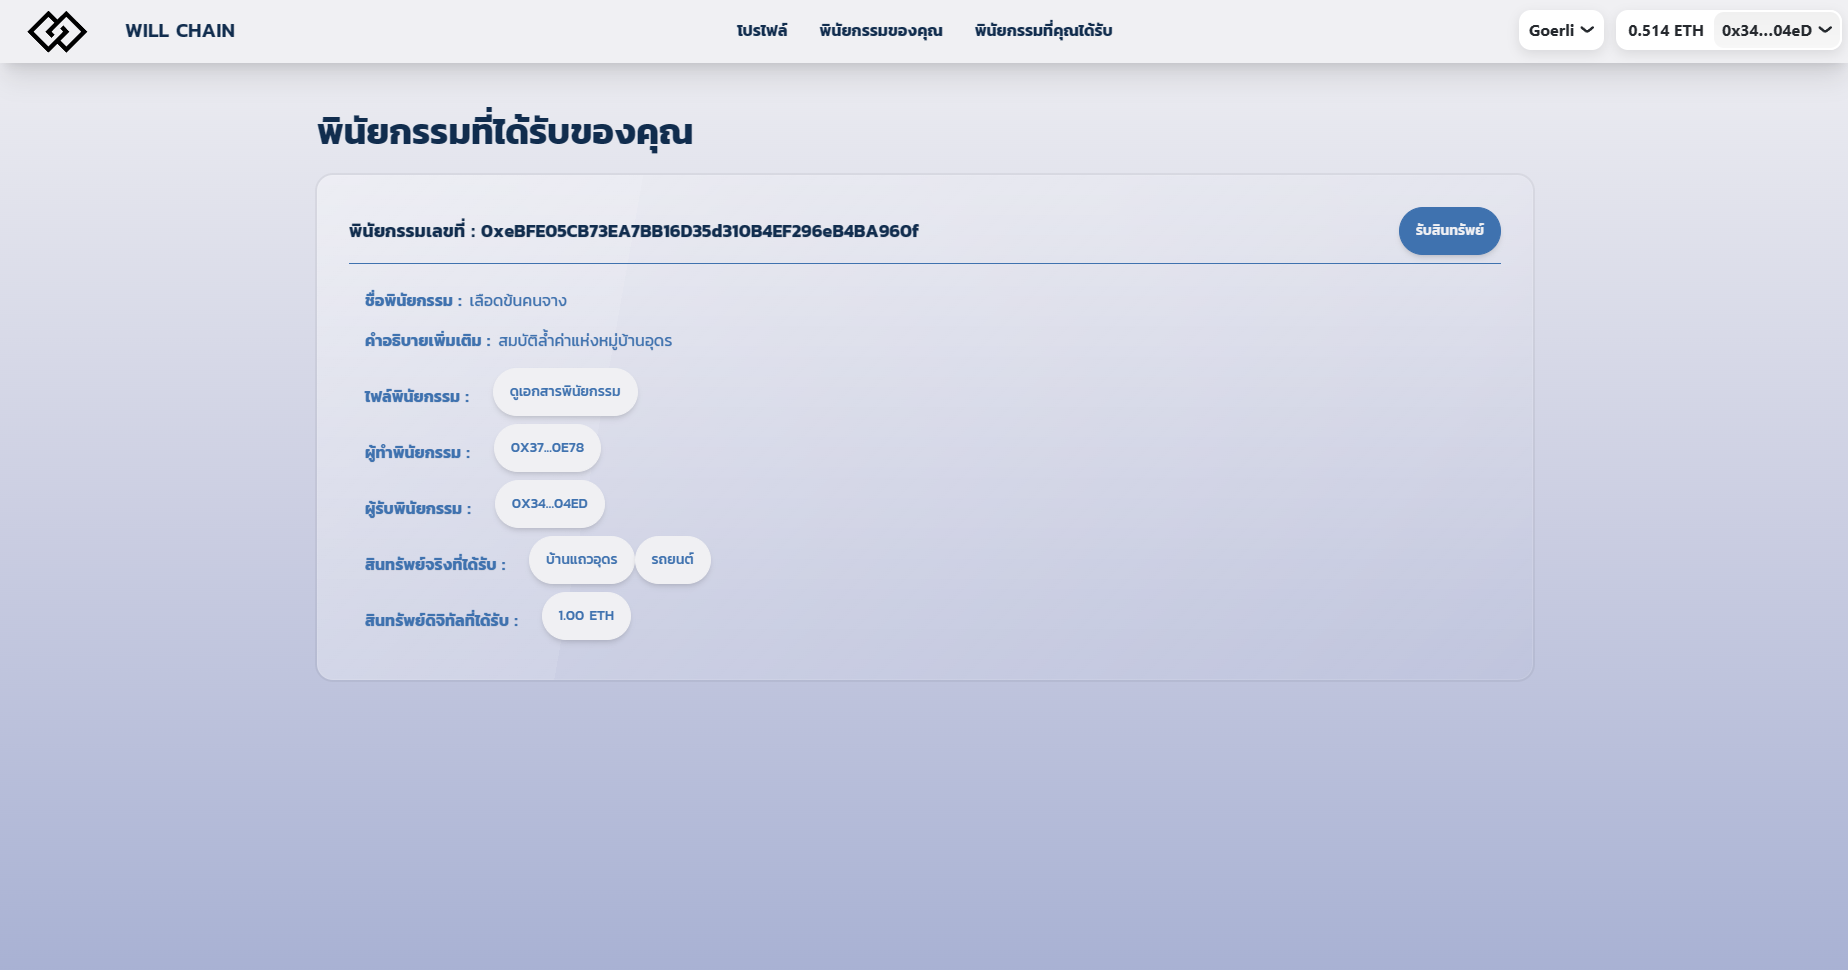
\includegraphics[scale=0.2]{claimWillBefore4}
			\caption{Beneficiary Claim Will Page }
		\end{figure}
		\FloatBarrier
\tab จากรูป จะแสดงหน้าเมื่อผู้ได้รับพินัยกรรมได้รับพินัยกรมม โดยระบบจะแสดงรายละเอียดของพินัยกรรมที่ได้รับพร้อมทั้งสินทรัพย์ที่แนบมาด้วย โดนจะมีปุ่มรับสินทรัพย์ให้ผู้ใช้งานกดเพื่อรับพินัยกรรมพร้อมสินทรพย์ที่แนบมา


\clearpage
\subsection{Beneficiary confirm claim will Page}
	\begin{figure}[!thb]
			\centering
			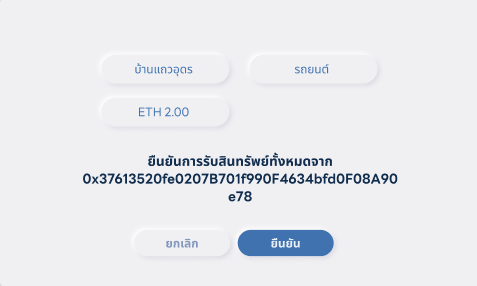
\includegraphics[scale=0.3]{claimWillConfirm4}
			\caption{Beneficiary Confirm Claim Will Modal }
		\end{figure}
		\FloatBarrier
\tab จากรูป หลังจากผู้ใช้งานกดปุ่มรับสินทรัพย์จะมี modal ให้ผู้ใช้งานทำการยืนยันเจตจำนงในการรับพินัยกรรม โดยจะมีปุ่มให้ผู้ใช้กดยืนยันเพื่อรับพินัยกรรมและปุ่มกดยกเลิกเมื่อยังไม่ต้องการรับพินัยกรรม

\subsection{Beneficiary Claim Will Page (succeed) }
	\begin{figure}[!thb]
			\centering
			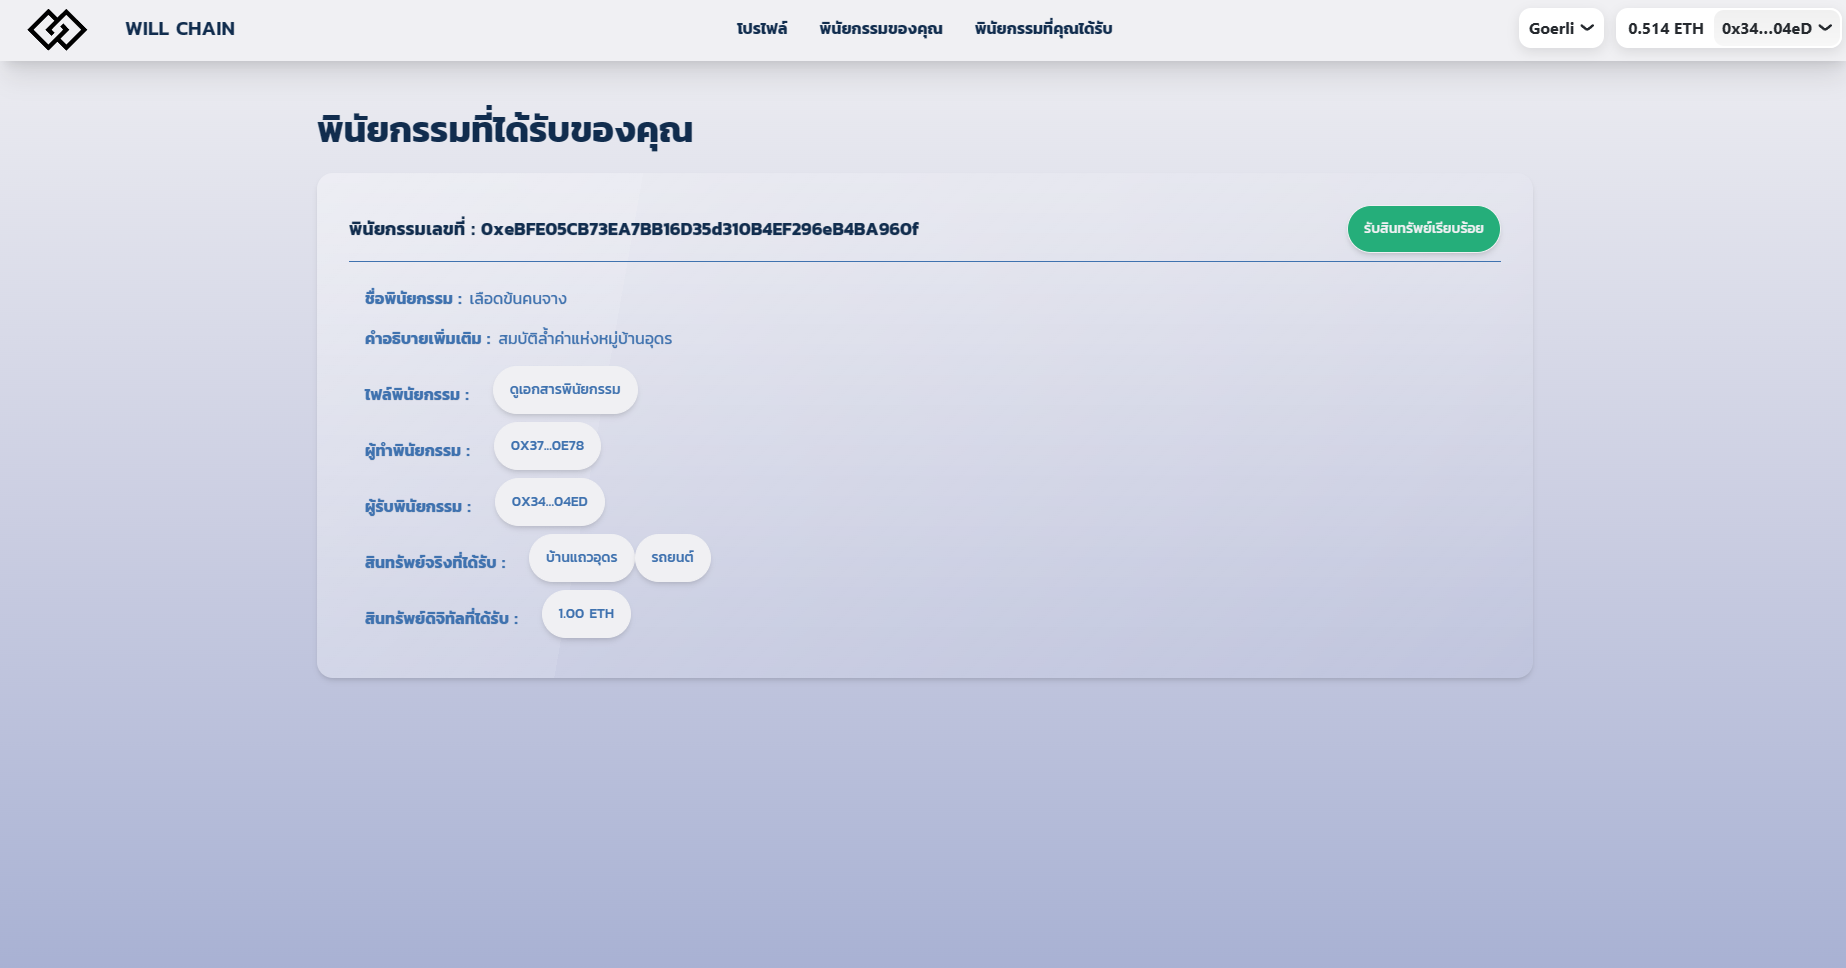
\includegraphics[scale=0.2]{claimWillSuc4}
			\caption{Beneficiary Claim Will Page (succeed)}
		\end{figure}
		\FloatBarrier
\tab จากรูป หลังจากผู้ใช้งานทำการรับพินัยกรรมแล้ว จะมีการแสดงสถานะของพินัยกรรมว่าผู้ใช้ได้ทำการรับสินทรัพย์เรียบร้อย

\clearpage
\section{Software Testing}
\tab System Testing จะใช้การทำ Unit Testing โดยทำการแยกการทดสอบเป็น function ต่าง ๆ ดังนี้
\subsection {Test Plan}
\begin{table}[h]
\begin{tabular}{|l|l|l|}
\hline
\multicolumn{1}{|c|}{\textbf{\centering หน้า}} & \multicolumn{1}{c|}{\textbf{\centering กรณีทดสอบ}} & \multicolumn{1}{c|}{\textbf{\centering ผลลัพท์}} \\
\hline
 หน้าโปรไฟล์           & ใส่รหัสบัตรประชาชนถูกต้อง                        &    \multicolumn{1}{c|}{{\color[HTML]{228B22} ผ่าน}} \\ \hline
                       & ใส่รหัสบัตรประชาชนไม่ครบ/เกิน                    &   \multicolumn{1}{c|}{{\color[HTML]{228B22} ผ่าน}}     \\ \hline
                       & เลือกเมนู Profile                            &   \multicolumn{1}{c|}{{\color[HTML]{228B22} ผ่าน}}      \\ \hline
                       & เลือกเมนู พินัยกรรมของคุณ                     &    \multicolumn{1}{c|}{{\color[HTML]{228B22} ผ่าน}}    \\ \hline
                       & เลือกเมนู  พินัยกรรมที่ได้รับ                    &   \multicolumn{1}{c|}{{\color[HTML]{228B22} ผ่าน}}     \\ \hline
หน้าพินัยกรรมของคุณ        & เลือกเพิ่มพินัยกรรม                              &   \multicolumn{1}{c|}{{\color[HTML]{228B22} ผ่าน}}    \\ \hline
                       & เลือกลบพินัยกรรม                                 &     \multicolumn{1}{c|}{{\color[HTML]{228B22} ผ่าน}}   \\ \hline
                       & เลือกจัดการพินัยกรรม                           &  \multicolumn{1}{c|}{{\color[HTML]{228B22} ผ่าน}}     \\ \hline
หน้าบันทึกพินัยกรรม        & กรอกข้อมูลครบทุกช่องแล้วกดบันทึก                   & \multicolumn{1}{c|}{{\color[HTML]{228B22} ผ่าน}}        \\ \hline
                       & ไม่กรอกชื่อพินัยกรรมแล้วขึ้นแจ้งเตือนให้ใส่ข้อมูล                      & \multicolumn{1}{c|}{{\color[HTML]{228B22} ผ่าน}}       \\ \hline
                       & ไม่อัพโหลดไฟล์พินัยกรรมแล้วขึ้นแจ้งเตือนให้ใส่ข้อมูล                      &      \multicolumn{1}{c|}{{\color[HTML]{228B22} ผ่าน}}  \\ \hline
                       & ไม่เพิ่มกระเป๋า wallet ของผู้ได้รับมรดกแล้วแจ้งเตือนให้ใส่ข้อมูล        & \multicolumn{1}{c|}{{\color[HTML]{228B22} ผ่าน}}        \\ \hline             
                       & กดปุ่มล้างข้อมูล แล้วล้างข้อมูลในฟอร์มที่กรอกมา       & \multicolumn{1}{c|}{{\color[HTML]{228B22} ผ่าน}}        \\ \hline                    
หน้าจัดการพินัยกรรม        & เลือกเพิ่มสินทรัพย์                              & \multicolumn{1}{c|}{{\color[HTML]{228B22} ผ่าน}}  \\ \hline                
หน้าเพิ่มสินทรัพย์จริง        & กรอกข้อมูลครบทุกช่องแล้วกดบันทึก                      &   \multicolumn{1}{c|}{{\color[HTML]{228B22} ผ่าน}}  \\ \hline
                       & ไม่กรอกชื่อสินทรัพย์แล้วขึ้นแจ้งเตือนให้ใส่ข้อมูล                                &  \multicolumn{1}{c|}{{\color[HTML]{228B22} ผ่าน}}     \\ \hline
                       & ไม่กรอกคำอธิบายแล้วขึ้นแจ้งเตือนให้ใส่ข้อมูล                          &    \multicolumn{1}{c|}{{\color[HTML]{228B22} ผ่าน}}   \\ \hline
                       & ไม่อัพโหลดไฟล์สินทรัพย์แล้วขึ้นแจ้งเตือนให้ใส่ข้อมูล                       & \multicolumn{1}{c|}{{\color[HTML]{228B22} ผ่าน}}      \\ \hline                    
                        & กดปุ่มล้างข้อมูล แล้วล้างข้อมูลในฟอร์มที่กรอกมา       & \multicolumn{1}{c|}{{\color[HTML]{228B22} ผ่าน}}        \\ \hline        
หน้าพินัยกรรมที่ได้รับ & กดปุ่มรับสินทรัพย์                              & \multicolumn{1}{c|}{{\color[HTML]{228B22} ผ่าน}}      \\ \hline
                       & เลือกยกเลิก                           &    \multicolumn{1}{c|}{{\color[HTML]{228B22} ผ่าน}}    \\ \hline
                       & เลือกยืนยัน                     & \multicolumn{1}{c|}{{\color[HTML]{228B22} ผ่าน}}      \\ \hline
\end{tabular}
\end{table}
\tab หลังจากผ่านการทำ System testing แล้วจะนำไปให้ User ทำการทดสอบว่าตอบสนองความต้องการหรือไม่ โดยจะนำไปให้บุคคลที่มี สินทรัพย์ดิจิทัลที่มีความต้องการที่จะทำพินัยกรรมทดลองใช้ Will Chain ของเรา

\begin{itemize}
	\item ความง่ายในการใช้งาน
	\item ความน่าเชื่อถือของ Software
	\item ความเสถียรของ Software
\end{itemize}
\clearpage

\subsection{Test Case}
\subsubsection{การทดสอบการเชื่อมต่อ Crypto Wallet}
\begin{table}[htbp]
\resizebox{\columnwidth}{!}{%
  \begin{tabular}{|l|l|l|l|}
  \hline
  \multicolumn{1}{|c|}{\textbf{รายละเอียดการทดสอบ}} & \multicolumn{1}{c|}{\textbf{ขั้นตอนการทดสอบ}} & \multicolumn{1}{c|}{\textbf{ผลลัพท์ที่คาดหวัง}} & \multicolumn{1}{c|}{\textbf{ผลการทดสอบ}} \\ \hline
  ทดสอบว่าผู้ใช้งานสามารถทำการเชื่อมต่อ crypto wallet & \begin{tabular}[l]{@{}l@{}}1.กดปุ่ม connect wallet\\ 2.ทำการเลือกชนิด crypto wallet\\ 3.เลือกบัญชี crypto wallet\end{tabular} & สามารถเชื่อมต่อ crypto wallet ได้ & \multicolumn{1}{c|}{{\color[HTML]{228B22} ผ่าน}} \\ \hline
  \end{tabular}%
}
\end{table}
\FloatBarrier

\subsubsection{การทดสอบการสร้างพินัยกรรม}
\FloatBarrier
\begin{table}[htbp]
\resizebox{\columnwidth}{!}{%
  \begin{tabular}{|l|l|l|l|}
  \hline
  \multicolumn{1}{|c|}{\textbf{รายละเอียดการทดสอบ}} & \multicolumn{1}{c|}{\textbf{ขั้นตอนการทดสอบ}} & \multicolumn{1}{c|}{\textbf{ผลลัพท์ที่คาดหวัง}} & \multicolumn{1}{c|}{\textbf{ผลการทดสอบ}} \\ \hline
ทดสอบว่าผู้ใช้งานสามารถสร้างพินัยกรรมได้ & \begin{tabular}[c]{@{}l@{}}1.กดปุ่ม บันทึกพินัยกรรม\\ 2.ใส่ชื่อพินัยกรรม\\ 3.อัพโหลดไฟล์พินัยกรรม\\ 4.กดบันทึกข้อมูล\end{tabular} & พินัยกรรมถูกบันทึกเข้าระบบ               & \multicolumn{1}{c|}{{\color[HTML]{228B22} ผ่าน}}     \\ \hline
ทดสอบปุ่มล้างข้อมูล                      & \begin{tabular}[c]{@{}l@{}}1.ทำการกรอกข้อมูลพินัยกรรม\\ 2.กดปุ่มล้างข้อมูล\end{tabular}                                           & ข้อมูลพินัยกรรมที่กรอกถูกลบ              & \multicolumn{1}{c|}{{\color[HTML]{228B22} ผ่าน}}     \\ \hline
ทดสอบการตรวจการกรอกข้อมูล (ชื่อ)               & 1.ไม่กรอกชื่อพินัยกรรม                                                                                                            & ขึ้นแจ้งเตือน "กรุณากรอกข้อมูลในช่องนี้" & \multicolumn{1}{c|}{{\color[HTML]{228B22} ผ่าน}}     \\ \hline
ทดสอบการตรวจการกรอกข้อมูล (ไฟล์)                                  & 1.ไม่อัพโหลดไฟล์พินัยกรรม                                                                                                         & ขึ้นแจ้งเตือน "กรุณาเลือกแฟ้ม"           & \multicolumn{1}{c|}{{\color[HTML]{228B22} ผ่าน}}     \\ \hline
\end{tabular}}
\end{table}
\FloatBarrier

\subsubsection{การทดสอบการ approve พินัยกรรม}
\begin{table}[htbp]
\resizebox{\columnwidth}{!}{%
  \begin{tabular}{|l|l|l|l|}
  \hline
  \multicolumn{1}{|c|}{\textbf{รายละเอียดการทดสอบ}} & \multicolumn{1}{c|}{\textbf{ขั้นตอนการทดสอบ}} & \multicolumn{1}{c|}{\textbf{ผลลัพท์ที่คาดหวัง}} & \multicolumn{1}{c|}{\textbf{ผลการทดสอบ}} \\ \hline
ทดสอบว่าผู้ใช้งานสามารถ approve พินัยกรรมได้ & \begin{tabular}[c]{@{}l@{}}1.กดปุ่ม ทำการ approve\\ 2.มีหน้า pop up แจ้งเตือนการ approve พินัยกรรม\\ 3..กดปุ่มยืนยัน บนหน้า pop up ที่แจ้งเตือนขึ้นมา\end{tabular} &พินัยกรรมถูก approve& \multicolumn{1}{c|}{{\color[HTML]{228B22} ผ่าน}} \\ \hline
\end{tabular}}
\end{table}
\FloatBarrier
\clearpage
\subsubsection{การทดสอบการจัดการพินัยกรรม}
\begin{table}[htbp]
\resizebox{\columnwidth}{!}{%
  \begin{tabular}{|l|l|l|l|}
  \hline
  \multicolumn{1}{|c|}{\textbf{รายละเอียดการทดสอบ}} & \multicolumn{1}{c|}{\textbf{ขั้นตอนการทดสอบ}} & \multicolumn{1}{c|}{\textbf{ผลลัพท์ที่คาดหวัง}} & \multicolumn{1}{c|}{\textbf{ผลการทดสอบ}} \\ \hline
ทดสอบว่าผู้ใช้งานสามารถจัดการพินัยกรรมได้ & \begin{tabular}[c]{@{}l@{}}1.กดปุ่ม จัดการพินัยกรรม\\ 2.ใส่เลข public keyของคนที่ได้รับสินทรัพย์\\ 3.เลือกสินทรัพย์ที่ต้องการแนบในพินัยกรรม\\ 4.ทำการบันทึกข้อมูล\end{tabular} & พินัยกรรมถูกจัดการ                      & \multicolumn{1}{c|}{{\color[HTML]{228B22} ผ่าน}}     \\ \hline
ทดสอบการตรวจการกรอกข้อมูล(public key)                 & 1.ไม่กรอกเลข public key ของคนที่ได้รับสินทรัพย์                                                                                                                                        & ขึ้นแจ้งเตือน"กรุณากรอกข้อมูลในช่องนี้" & \multicolumn{1}{c|}{{\color[HTML]{228B22} ผ่าน}}     \\ \hline

\end{tabular}}
\end{table}
\FloatBarrier

\subsubsection{การทดสอบการยกเลิกพินัยกรรม}
\begin{table}[htbp]
\resizebox{\columnwidth}{!}{%
  \begin{tabular}{|l|l|l|l|}
  \hline
  \multicolumn{1}{|c|}{\textbf{รายละเอียดการทดสอบ}} & \multicolumn{1}{c|}{\textbf{ขั้นตอนการทดสอบ}} & \multicolumn{1}{c|}{\textbf{ผลลัพท์ที่คาดหวัง}} & \multicolumn{1}{c|}{\textbf{ผลการทดสอบ}} \\ \hline
ทดสอบว่าผู้ใช้งานสามารถยกเลิกพินัยกรรมได้ & \begin{tabular}[c]{@{}l@{}}1.กดปุ่ม ยกเลิกพินัยกรรม\\ 2.กดปุ่มยืนยันบน pop up ที่แจ้งเตือนขึ้นมา\end{tabular} & พินัยกรรมถูกยกเลิก & \multicolumn{1}{c|}{{\color[HTML]{228B22} ผ่าน}} \\ \hline
\end{tabular}}
\end{table}
\FloatBarrier

\subsubsection{การทดสอบการรับสินทรัพย์จากพินัยกรรม}
\begin{table}[htbp]
\resizebox{\columnwidth}{!}{%
  \begin{tabular}{|l|l|l|l|}
  \hline
  \multicolumn{1}{|c|}{\textbf{รายละเอียดการทดสอบ}} & \multicolumn{1}{c|}{\textbf{ขั้นตอนการทดสอบ}} & \multicolumn{1}{c|}{\textbf{ผลลัพท์ที่คาดหวัง}} & \multicolumn{1}{c|}{\textbf{ผลการทดสอบ}} \\ \hline
ทดสอบว่าผู้ใช้งานรับสินทรัพย์จากพินัยกรรมได้ & \begin{tabular}[c]{@{}l@{}}1.กดปุ่ม พินัยกรรมที่คุณได้รับ\\ 2.กดปุ่ม รับสินทรัพย์\end{tabular} & \begin{tabular}[c]{@{}l@{}}พินัยกรรมถูกรับ\end{tabular} & \multicolumn{1}{c|}{{\color[HTML]{228B22} ผ่าน}} \\ \hline
\end{tabular}}
\end{table}
\FloatBarrier
\clearpage

\subsection {Test Smart Contract}
\subsubsection { การทดสอบ Smart Contract ด้วย Hardhat Testing}
	\tab\tab การทดสอบด้วย Hardhat Testing ผู้จัดทำได้ออกแบบการทดสอบของ Smart Contract ด้วยแบ่งเป็น Flow ในการเรียกใช้งานในแต่ละ Test Case เพื่อให้ครอบคลุมทุกเงื่อนไขในแต่ละฟังก์ชัน
\begin{figure}[!thb]
			\centering
			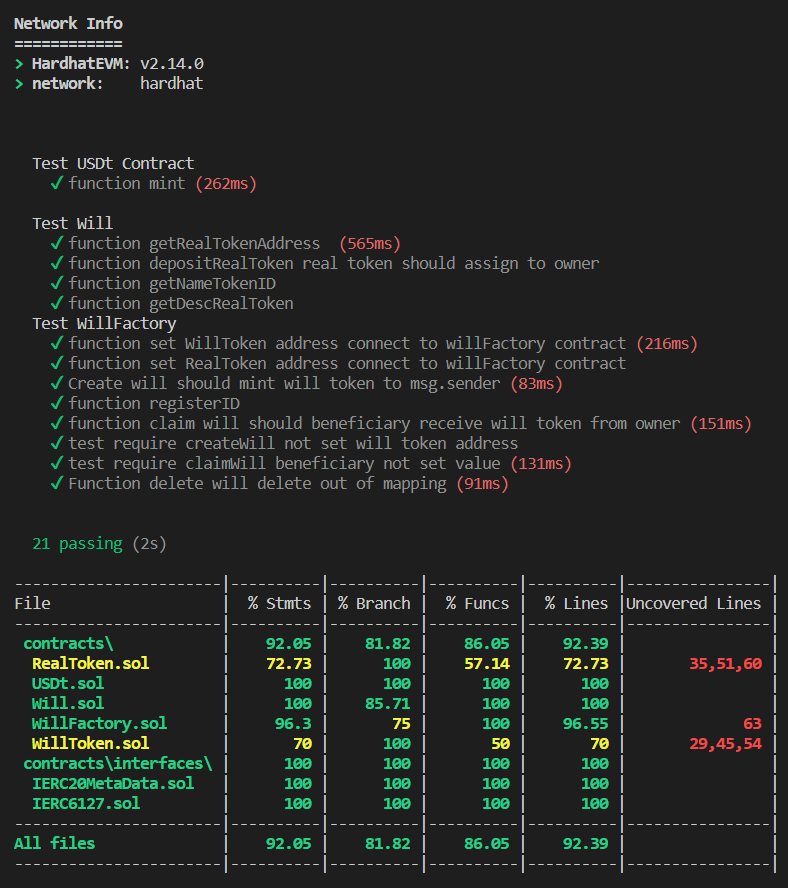
\includegraphics[scale=0.5]{testCoverage}
			\caption{ผล Test Coverage ของ Smart Contract}
		\end{figure}
\FloatBarrier
\tab จากรูป เป็นการออกแบบ Test Case ให้ครอบคลุมทุกฟังก์ชันโดยจากภาพจะมีค่า Test Coverage โดย \\ \tab\%Stmts เป็นตัวชี้วัดวัดเปอร์เซ็นต์ของคำสั่งรหัสที่ถูกดำเนินการในระหว่างการทดสอบ ระบุจำนวนบรรทัดของ code ที่ถูกเรียกใช้อย่างน้อยหนึ่งครั้ง \\ \tab\%Branch เป็นตัวชี้วัดวัดเปอร์เซ็นต์ของ code ที่ได้รับระหว่างการทดสอบ ตรวจสอบโดยเป็นการตรวจสอบเงื่อนไขของตัว Smart Contract  \\ \tab\%Funcs เป็นตัวชี้วัดเปอร์เซ็นต์ของฟังก์ชันที่ถูกเรียกใช้ในระหว่างการทดสอบ จะตรวจสอบว่าแต่ละฟังก์ชันได้รับการดำเนินการอย่างน้อยหนึ่งครั้งหรือไม่  \\\tab\%Lines เป็นตัวชี้วัดเปอร์เซ็นต์ของความครอบคลุมของบรรทัดของ code โดยจะวัดเปอร์เซ็นต์ของบรรทัดโค้ดที่ดำเนินการระหว่างการทดสอบ

\section{การ Deploy Smart Contract ไปที่ Ethereum Chain}
	\tab การ Deploy Smart Contract ไปที่ Ethereum Chain โดยเป็น Test network เพื่อความรวดเร็วในการ Deploy Smart Contract และไม่มีค่าธรรมเนียมในการทำธุรกรรมต่าง ๆ ในการทำงานของระบบ โดยใช้ Hardhat ในการทำการ Deploy Smart Contract โดยมีขั้นตอนดังนี้
	\\\tab 1. ต้องทำการ Deploy Contract WillFactory ซึ่งเป็น Contract ที่ใช้สำหรับการจัดการพินัยกรรมทั้งหมดและจัดการการสืบทอดพินัยกรรมของพินัยกรรมทั้งหมด
	\\\tab 2. ทำการ Deploy Contract Will Token เพื่อที่จะทำการสร้างพินัยกรรมและเป็น NFT มาตรฐาน ERC-721 โดย Will Token ไม่สามารถถ่ายโอนให้คนอื่นได้ด้วยตัวเอง แต่จะสามารถถ่ายโอนได้ ผ่าน Contract WillFactory เท่านั้น
	\\\tab 3. ทำการ Deploy Contract Real Token เพื่อที่จะทำการนำสินทรัพย์จริงไปสร้างเป็น NFT มาตรฐาน ERC-721 โดย Real Token จะไม่สามารถถ่ายโอนให้คนอื่นได้ด้วยตัวเอง แต่จะสามารถถ่ายโอนได้ ผ่าน Contract Will เท่านั้น
	\\\tab 4. ทำการ Deploy Contract USDt เพื่อที่จะทำการจำลองสินทรัพย์ดิจิทัลประเภทเหรียญในระบบ โดยจะเป็นมาตรฐาน ERC-20 ใช้สำรองทดสอบการฝากด้วย Token ที่นอกเหนือจาก ETH
	\\\tab 5. ทำการ Deploy Contract Will เป็นการ Contract ที่สร้างขึ้นมาจาก Will Factory โดย Will Contract จะทำหน้าที่ค่อยเก็บพินัยกรรมของเจ้าของพินัยกรรมและจัดการพินัยกรรมสินทรัพย์ในระบบทั้งหมด
\\\tab 	ผลลัพท์ของการ Deploy Smart Contract จะได้ Contract Address ดังนี้
\\\tab willFactory deployed to: 0x54BeBcd2469AAE5E4417f4c6d01d2C8Eb31331cC
\\\tab willToken deployed to: 0x9f2c24a6aB735C9ECFbF2e8d1A36CD8F54D2248F 
\\\tab USDt deployed to: 0xe25ddff621198069bA7fe5A18f3D94C1f6F60496 
\\\tab RealToken deployed to: 0x7d7Ce3e5Be7Be44FC38F9A73046D2d79735d552f
\\\tab โดย Will Contract จะถูกสร้างด้วย WillFactory และ Smart Contract ทั้งหมดจะถูก verify เพื่อความถูกต้องและความปลอดภัยด้วย Hardhat verify โดย Smart Contract ที่ verify แล้วจะแสดงผลได้ที่หน้า Etherscan ที่เป็น block explorer และ สามารถใช้ฟังก์ชั่นใน Contract  ได้ผ่าน หัวข้อ Contract 
\begin{figure}[!thb]
			\centering
			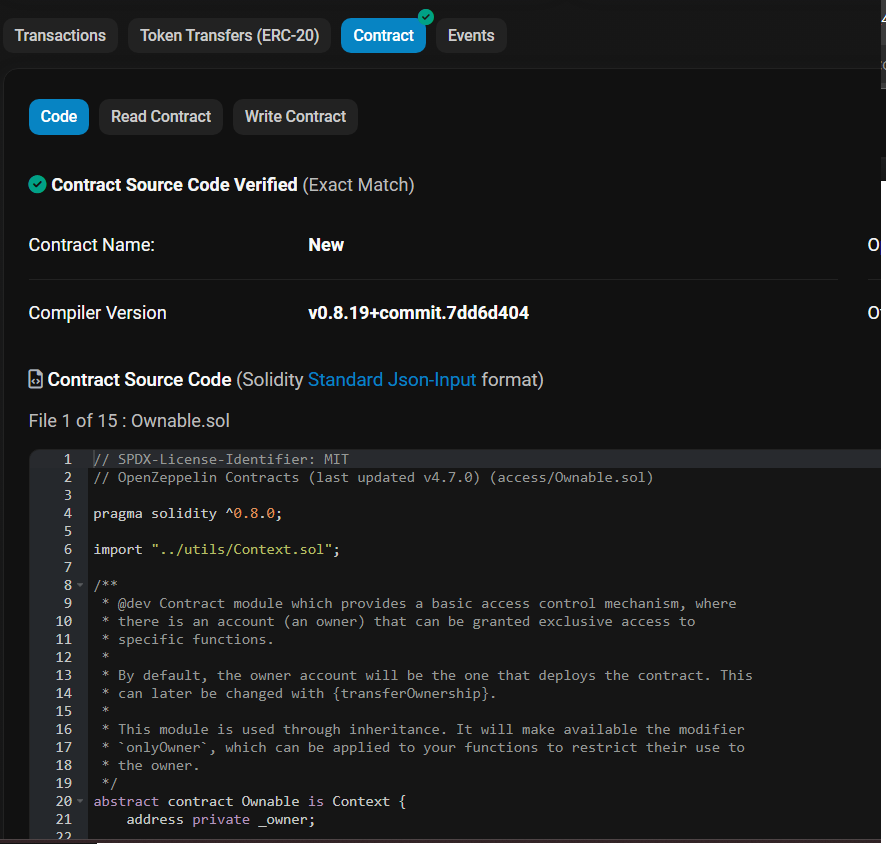
\includegraphics[scale=0.5]{etherscan}
			\caption{แสดงผล code หลัง verified contract}
		\end{figure}
\begin{figure}[!thb]
			\centering
			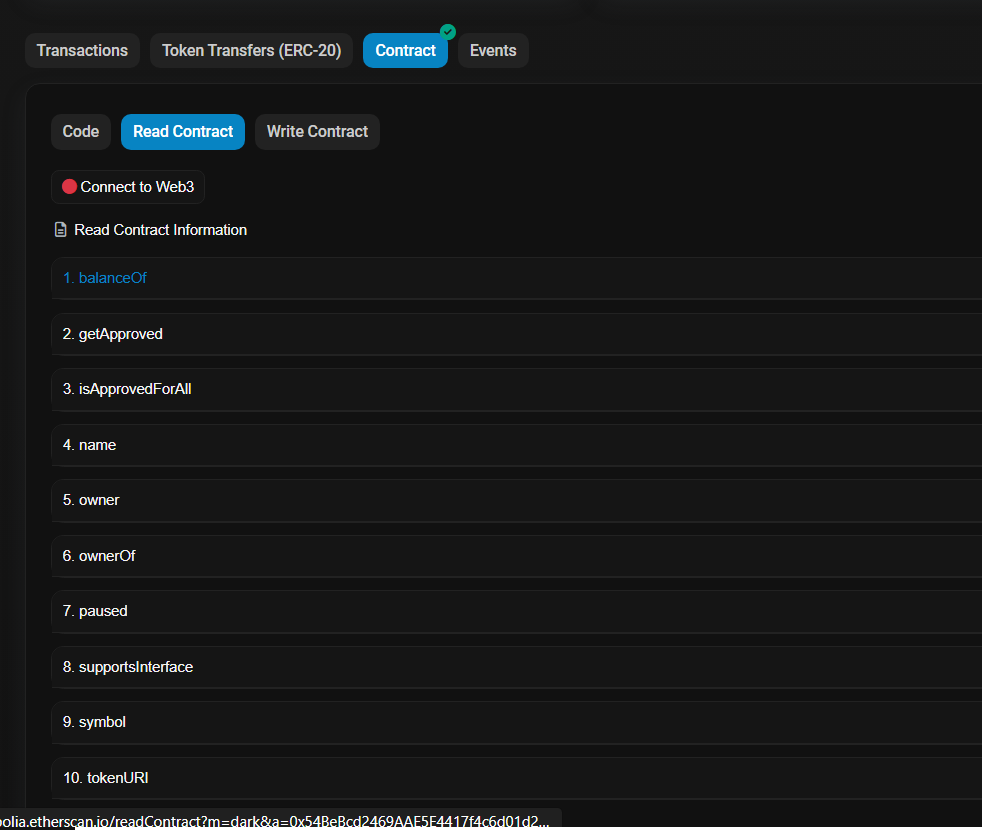
\includegraphics[scale=0.5]{etherscanRead}
			\caption{แสดงฟังก์ชั่นสำหรับที่แสดงผล หลัง verified contract}
		\end{figure}
\begin{figure}[!thb]
			\centering
			\includegraphics[scale=0.5]{etherscanWrite}
			\caption{แสดงฟังก์ชั่นที่มีการเขียนลงระบบ Ethereum chain หลัง verified contract}
		\end{figure}
\chapter{สรุปผล}
\section{ สรุปปัญหาที่พบและวิธีการแก้ไข}
\subsection{Blockchain}
\tab ปัญหาที่พบ 1 : ไม่มี Token ของสินทรัพย์ดิจิทัลให้ทดสอบกับตัว Contract \\
\tab การแก้ไข : เลือกใช้วิธีการสร้าง Contract USDt ซึ่งเป็นเหรียญที่ใช้ interface ตัวเดียวกันกับของที่มีอยู่ใน ฺBlockchain
\subsection{Smart Contract}
\tab การแก้ไข : ทำการใช้ interface AccesControl เป็นตัวช่วยในการจัดการ Role และ เพิ่ม role ของ Smart Contract\\
\tab ปัญหาที่พบ 1 : มีปัญหาเรื่องการการ estimate gas ไม่ได้ ตอนที่ทำการ Transfer จาก Will Contract ไปที่กระเป๋าของผู้รับพินัยกรรม\\
\tab การแก้ไข : ทำการ approve token ของเจ้าของพินัยกรรมนั้นก่อนทำการส่งไปที่ Contract\\
\tab ปัญหาที่พบ 2 : ไม่สามารถใช้งาน API เช็คการเสียชีวิตจากกรมการปกครองได้\\
\tab การแก้ไข : ทำการ Assume ส่วน API เช็คการเสียชีวิตแทนด้วย AccessControl เป็น Role Controller เพื่อทำการ Control การเสียชีวิตของผู้ทำพินัยกรรม
\subsection{Frontend}
\tab ปัญหาที่พบ 1 : ทำการเชื่อมต่อ MetaMask Wallet กับ frontend ได้ยุ่งยาก\\
\tab การแก้ไข : ทำการใช้ตัว thirdparty ในการเชื่อมต่อกับ MetaMask Wallet\\
\tab ปัญหาที่พบ 2 : การ integrate frontend กับ Smart Contract นั้นใช้ระยะเวลาที่นานในการทำ เพราะ ขาดความรู้ในเรื่อง Web3 และการเชื่อมต่อกับ Smart Contract\\
\tab การแก้ไข : แบ่งเวลามาศึกษาเพิ่มมากยิ่งขึ้น

\clearpage
\section{สถานะการดำเนินงาน}
\tab จากการดำเนินโครงการตั้งแต่ภาคการศึกษาที่ 1 ถึง ภาคการศึกษาที่ 2 ประจำปีการศึกษา 2565 แบ่งสถานะการดำเนินการออกเป็น 3 รูปแบบ คือ เสร็จสมบูรณ์ อยู่ระหว่างการพัฒนา พัฒนาต่อในอนาคต โดยในแต่ละการดำเนินงาน แสดงดังตาราง

% Please add the following required packages to your document preamble:
% \usepackage{multirow}
% \usepackage{graphicx}
% \usepackage[table,xcdraw]{xcolor}
% If you use beamer only pass "xcolor=table" option, i.e. \documentclass[xcolor=table]{beamer}
\begin{table}[h]
\centering
\caption{ตารางสรุปผลการดำเนินงาน}
\label{tab:op-table}
\resizebox{\textwidth}{!}{%
\begin{tabular}{|lllll|}
\hline
\multicolumn{1}{|c|}{} &
  \multicolumn{3}{c|}{\textbf{ผลดำเนินงาน}} &
  \multicolumn{1}{c|}{} \\ \cline{2-4}
\multicolumn{1}{|c|}{\multirow{-2}{*}{\textbf{การดำเนินงาน}}} &
  \multicolumn{1}{c|}{\textbf{เสร็จสมบูรณ์}} &
  \multicolumn{1}{c|}{\textbf{อยู่ระหว่างการพัฒนา}} &
  \multicolumn{1}{c|}{\textbf{พัฒนาต่อในอนาคต}} &
  \multicolumn{1}{c|}{\multirow{-2}{*}{\textbf{ผู้รับผิดชอบ}}} \\ \hline
\multicolumn{1}{|l|}{\textbf{การศึกษาความต้องการในการออกแบบเว็บไซต์}} &
  \multicolumn{1}{l|}{\cellcolor[HTML]{25AE7A}} &
  \multicolumn{1}{l|}{} &
  \multicolumn{1}{l|}{} &
  ฐิติพงศ์, ณรงค์ยศ, ทรัพย์ทวี \\ \hline
\multicolumn{1}{|l|}{\textbf{การออกแบบโครงสร้างของระบบ}} &
  \multicolumn{1}{l|}{\cellcolor[HTML]{25AE7A}{\color[HTML]{32CB00} }} &
  \multicolumn{1}{l|}{} &
  \multicolumn{1}{l|}{} &
  ฐิติพงศ์, ณรงค์ยศ, ทรัพย์ทวี \\ \hline
\multicolumn{1}{|l|}{\textbf{การออกแบบส่วนติดต่อผู้ใข้งาน}} &
  \multicolumn{1}{l|}{\cellcolor[HTML]{25AE7A}{\color[HTML]{32CB00} }} &
  \multicolumn{1}{l|}{} &
  \multicolumn{1}{l|}{} &
  ฐิติพงศ์, ณรงค์ยศ \\ \hline
\multicolumn{5}{|l|}{\textbf{การพัฒนาส่วนติดต่อผู้ใช้งาน (Web3)}} \\ \hline
\multicolumn{1}{|l|}{\begin{tabular}[c]{@{}l@{}}หน้าแรกของเว็บไซต์\\ (Home page)\end{tabular}} &
  \multicolumn{1}{l|}{\cellcolor[HTML]{25AE7A}} &
  \multicolumn{1}{l|}{} &
  \multicolumn{1}{l|}{} &
  ณรงค์ยศ \\ \hline
\multicolumn{1}{|l|}{\begin{tabular}[c]{@{}l@{}}หน้าโปรไฟล์\\ (Profile page)\end{tabular}} &
  \multicolumn{1}{l|}{\cellcolor[HTML]{25AE7A}} &
  \multicolumn{1}{l|}{} &
  \multicolumn{1}{l|}{} &
  ณรงค์ยศ \\ \hline
\multicolumn{1}{|l|}{\begin{tabular}[c]{@{}l@{}}หน้าพินัยกรรมที่บันทึกของคุณ\\ (My will page)\end{tabular}} &
  \multicolumn{1}{l|}{\cellcolor[HTML]{25AE7A}} &
  \multicolumn{1}{l|}{} &
  \multicolumn{1}{l|}{} &
  ณรงค์ยศ \\ \hline
\multicolumn{1}{|l|}{\begin{tabular}[c]{@{}l@{}}หน้าบันทึกพินัยกรรม\\ (Create will page)\end{tabular}} &
  \multicolumn{1}{l|}{\cellcolor[HTML]{25AE7A}} &
  \multicolumn{1}{l|}{} &
  \multicolumn{1}{l|}{} &
  ณรงค์ยศ \\ \hline
\multicolumn{1}{|l|}{\begin{tabular}[c]{@{}l@{}}หน้าจัดการพินัยกรรม\\ (Manage will page)\end{tabular}} &
  \multicolumn{1}{l|}{\cellcolor[HTML]{25AE7A}} &
  \multicolumn{1}{l|}{} &
  \multicolumn{1}{l|}{} &
  ณรงค์ยศ \\ \hline
\multicolumn{1}{|l|}{\begin{tabular}[c]{@{}l@{}}หน้าเพิ่มสินทรัพย์จริง\\ (Create Real Asset page)\end{tabular}} &
  \multicolumn{1}{l|}{\cellcolor[HTML]{25AE7A}} &
  \multicolumn{1}{l|}{} &
  \multicolumn{1}{l|}{} &
  ณรงค์ยศ \\ \hline
\multicolumn{1}{|l|}{\begin{tabular}[c]{@{}l@{}}หน้าพินัยกรรมที่ได้รับของคุณ\\ (Claim page)\end{tabular}} &
  \multicolumn{1}{l|}{\cellcolor[HTML]{25AE7A}} &
  \multicolumn{1}{l|}{} &
  \multicolumn{1}{l|}{} &
  ณรงค์ยศ \\ \hline
\multicolumn{1}{|l|}{Service IPFS metadata} &
  \multicolumn{1}{l|}{\cellcolor[HTML]{25AE7A}} &
  \multicolumn{1}{l|}{} &
  \multicolumn{1}{l|}{} &
  ทรัพย์ทวี \\ \hline
\multicolumn{5}{|l|}{\textbf{Smart Contract}} \\ \hline
\multicolumn{1}{|l|}{WillFactory contract} &
  \multicolumn{1}{l|}{\cellcolor[HTML]{25AE7A}} &
  \multicolumn{1}{l|}{} &
  \multicolumn{1}{l|}{} &
  ทรัพย์ทวี \\ \hline
\multicolumn{1}{|l|}{WillToken contract} &
  \multicolumn{1}{l|}{\cellcolor[HTML]{25AE7A}} &
  \multicolumn{1}{l|}{} &
  \multicolumn{1}{l|}{} &
  ทรัพย์ทวี \\ \hline
\multicolumn{1}{|l|}{Will contract} &
  \multicolumn{1}{l|}{\cellcolor[HTML]{25AE7A}} &
  \multicolumn{1}{l|}{} &
  \multicolumn{1}{l|}{} &
  ทรัพย์ทวี \\ \hline
\multicolumn{1}{|l|}{USDt contract} &
  \multicolumn{1}{l|}{\cellcolor[HTML]{25AE7A}} &
  \multicolumn{1}{l|}{} &
  \multicolumn{1}{l|}{} &
  ทรัพย์ทวี \\ \hline
\multicolumn{1}{|l|}{RealToken contract} &
  \multicolumn{1}{l|}{\cellcolor[HTML]{25AE7A}} &
  \multicolumn{1}{l|}{} &
  \multicolumn{1}{l|}{} &
  ทรัพย์ทวี \\ \hline
\multicolumn{5}{|l|}{\textbf{Backend}} \\ \hline
\multicolumn{1}{|l|}{ระบบตรวจสอบการเสียชีวิต} &
  \multicolumn{1}{l|}{} &
  \multicolumn{1}{l|}{} &
  \multicolumn{1}{l|}{\cellcolor[HTML]{C0C0C0}} &
  ทรัพย์ทวี \\ \hline
\multicolumn{5}{|l|}{\textbf{Storage}} \\ \hline
\multicolumn{1}{|l|}{IPFS metadata} &
  \multicolumn{1}{l|}{\cellcolor[HTML]{25AE7A}} &
  \multicolumn{1}{l|}{} &
  \multicolumn{1}{l|}{} &
  ทรัพย์ทวี \\ \hline
\multicolumn{5}{|l|}{\textbf{Deployment}} \\ \hline
\multicolumn{1}{|l|}{Deploy smart contract} &
  \multicolumn{1}{l|}{\cellcolor[HTML]{25AE7A}} &
  \multicolumn{1}{l|}{} &
  \multicolumn{1}{l|}{} &
  ทรัพย์ทวี \\ \hline
\multicolumn{1}{|l|}{Deploy website} &
  \multicolumn{1}{l|}{\cellcolor[HTML]{25AE7A}} &
  \multicolumn{1}{l|}{} &
  \multicolumn{1}{l|}{} &
  ณรงค์ยศ \\ \hline
\multicolumn{1}{|l|}{Verify smart contract} &
  \multicolumn{1}{l|}{\cellcolor[HTML]{25AE7A}} &
  \multicolumn{1}{l|}{} &
  \multicolumn{1}{l|}{} &
  ทรัพย์ทวี \\ \hline
\multicolumn{5}{|l|}{\textbf{การทดสอบระบบ}} \\ \hline
\multicolumn{1}{|l|}{Unit testing} &
  \multicolumn{1}{l|}{\cellcolor[HTML]{25AE7A}} &
  \multicolumn{1}{l|}{} &
  \multicolumn{1}{l|}{} &
  ฐิติพงศ์ \\ \hline
\multicolumn{1}{|l|}{Integration testing} &
  \multicolumn{1}{l|}{\cellcolor[HTML]{25AE7A}} &
  \multicolumn{1}{l|}{} &
  \multicolumn{1}{l|}{} &
  ฐิติพงศ์ \\ \hline
\multicolumn{1}{|l|}{Smart contract testing} &
  \multicolumn{1}{l|}{\cellcolor[HTML]{25AE7A}} &
  \multicolumn{1}{l|}{} &
  \multicolumn{1}{l|}{} &
  ทรัพย์ทวี \\ \hline
\end{tabular}%
}
\end{table}
\clearpage

\section{สรุปผลการดำเนินงาน}

\subsection{Will}
\tab สามารถแสดงผลของรายละเอียดพินัยกรรม โดยเปิดให้ผู้ใช้งานมาใช้ได้ด้วยการกรอกเลขบัตรประชาชนไปที่หน้า Profile สำหรับการลงทะเบียนเลขบัตรประชาชน หลังจากนั้นเจ้าของพินัยกรรมจะสามารถใช้งานระบบได้และมีการแสดงหน้าสำหรับให้ผู้ใช้สร้างพินัยกรรม และ สามารถเพิ่มสินทรัพย์ดิจิทัล ที่ใช้มาตรฐาน ERC-20 รวมถึงการทำ NFT ของสินทรัพย์จริงได้ โดยพินัยกรรมจะทำงานก็ต่อเมื่อมีการเสียชีวิตของผู้ทำพินัยกรรม โดยจะมี role ที่ทำการควบคุมคือ controller ซึ่งจะสามารถทำให้พินัยกรรมส่งไปหาผู้รับพินัยกรรมผ่านกระเป๋า MetaMask Wallet

\subsection{Will Token}
\tab สามารถแสดงผลของการทำ NFT ของตัวพินัยกรรม โดยตัว Will Token จะทำหน้าที่เป็นพินัยกรรมโดยถ้าผู้รับพินัยกรรมไม่ได้ถือเหรียญ Will Token ที่ผูกกับพินัยกรรมนั้น ก็จะไม่สามารถใช้งานพินัยกรรมในระบบหรือถอนสินทรัพย์ออกจากระบบได้
\subsection{Claim Assets}
\tab สามารถรับสินทรัพย์จากการที่ role controller ที่ควบคุมของการดำเนินการของการส่งพินัยกรรมก่อนจึงจะสามารถรับสินทรัพย์ในระบบได้ โดยสามารถรับสินทรัพย์ดิจิทัลที่ใช้มาตรฐาน ERC-20 และสามารถรับสินทรัพย์จริงในรูปแบบของ NFT ที่ถูกสร้างขึ้นจากสินทรัพย์จริงได้มาสู่ผู้รับพินัยกรรม

\subsection{แนวทางในการพัฒนาในอนาคต}
\tab แนวทางในการพัฒนาโครงงานต่อในอนาคตจะเกี่ยวข้องกับการติดต่อฝ่ายกรมการปกครองเพื่อใช้งาน API เพื่อตรวจสอบสถานะการเสียชีวิตและนำข้อมูลมาใช้ในระบบ นอกจากนี้ยังมีการใช้งาน Soulbound Token (SBT) เพื่อยืนยันตัวตนและเก็บข้อมูลผู้ใช้ในระบบ ทำให้สะดวกต่อการระบุตัวตน และมีการเพิ่มระบบ Multisig Wallet เพื่อให้ผู้ใช้สามารถเลือกที่จะไม่เก็บสินทรัพย์หรือทรัพย์สินใดๆ ในระบบ โดย Multisig Wallet จะเป็นการเลือกผู้รับมอบอำนาจที่สามารถอนุมัติกระเป๋าเงินหลักที่ถูกมอบหมายให้เป็นผู้ทำการมอบอำนาจ และผู้ใช้สามารถเลือกจำนวนผู้อนุมัติที่ต้องการสำหรับกระเป๋าเงินได้เอง\\
\tab ต่อมาคือฟีเจอร์สำหรับการเซ็นเอกสารออนไลน์ภายในระบบ ซึ่งผู้ใช้สามารถเซ็นเอกสารพินัยกรรมออนไลน์ได้ ในการทำพินัยกรรมจะครบถ้วนตามขั้นตอนและหลักเกณฑ์ที่ใช้ในชีวิตจริง และเพิ่มความน่าเชื่อถือ \\
\tab ต่อมาคือการต่อยอดในด้านของการเก็บเอกสารสำคัญเพิ่มเติมในระบบ Blockchain เพื่อเพิ่มความปลอดภัยและความน่าเชื่อถือ \\
\tab ต่อมาคือการต่อยอดเป็นฟีเจอร์การสืบทอดสินทรัพย์ดิจิทัลใน Exchange platform \\
%%%%%%%%%%%%%%%%%%%%%%%%%%%%%%%%%%%%%%%%%%%%%%%%%%%%%%%%%%%%%%%
%%%%%%%%%%%%%%%%%%%% Bibliography %%%%%%%%%%%%%%%%%%%%%%%%%%%%%
%%%%%%%%%%%%%%%%%%%%%%%%%%%%%%%%%%%%%%%%%%%%%%%%%%%%%%%%%%%%%%%

%%%% Comment this in your report to show only references you have
%%%% cited. Otherwise, all the references below will be shown.
%\nocite{*}
%% Use the kmutt.bst for bibtex bibliography style 
%% You must have cpe.bib and string.bib in your current directory.
%% You may go to file .bbl to manually edit the bib items.

\makeatletter
\g@addto@macro{\UrlBreaks}{\UrlOrds}
\makeatother

\bibliographystyle{kmutt}
\bibliography{string,cpe}
 \appendix{ผลแบบสอบถามจากการสำรวจ และศึกษาความต้องการของผู้ใช้งาน} 
\noindent{\large\bf ผลแบบสอบถามจากการสำรวจ และศึกษาความต้องการของผู้ใช้งาน} \\
\tab การศึกษาความต้องการและข้อมูลเชิงลึกเพื่อทราบความต้องการผู้ใช้งานระบบพินัยกรรมบนเครือข่ายบล็อกเชน  ด้วยการใช้การสำรวจหาพฤติกรรมของผู้ใช้ของสินทรัพย์ต่าง ๆ เพื่อทำให้การออกแบบมีความเหมาะสมและตรงตามวัตถุประสงค์ โดยแบบสำรวจประกอบด้วย 3 ส่วน คือ ข้อมูลทั่วไป คำถามสำคัญเพื่อการนำไปพัฒนาระบบพินัยกรรม และทางคณะผู้จัดทำโครงงานได้สร้างแบบสอบถามด้วย Google Form และกำหนดให้ตัวอย่างเป็นผู้มีความสนใจสินทรัพย์ดิจิทัล และ ไม่สนใจในสินทรัพย์ดิจิทัล โดยมีผู้ตอบแบบประเมินทั้งสิ้น 59 โดยแบ่งเป็นผู้มีความสนใจสินทรัพย์ 54 คน และไม่สนใจ 5 คน โดยเราจะนำข้อมูลของผู้มีความสนใจในสินทรัพย์มาทำการตอบแบบสอบถามเพิ่มเติม ดังนี้\\

\bf คำถามข้อที่ 1 คุณมีความสนใจในสินทรัพย์ดิจิทัล อย่าง Cryptocurrency , NFT หรือไม่

\begin{figure}[!thb]
			\centering
			\includegraphics[scale=0.3]{apprex1}
			\caption{ผลสำรวจแบบสอบถามของคำถามที่ 1}
		\end{figure}
\FloatBarrier
\bf คำถามข้อที่ 2 คุณมีสินทรัพย์ดิจิทัลอย่าง Cryptocurrency , NFT ในการครอบครองหรือไม่\\
\begin{figure}[!thb]
			\centering
			\includegraphics[scale=0.3]{apprex2}
			\caption{ผลสำรวจแบบสอบถามของคำถามที่ 2}
		\end{figure}
\FloatBarrier

\clearpage
\bf คำถามข้อที่ 3 เพศ (Gender)\\
\begin{figure}[!thb]
			\centering
			\includegraphics[scale=0.3]{apprex3}
			\caption{ผลสำรวจแบบสอบถามของคำถามที่ 3}
		\end{figure}
\FloatBarrier

\bf คำถามข้อที่ 4 อายุในปัจจุบัน\\
\begin{figure}[!thb]
			\centering
			\includegraphics[scale=0.3]{apprex4}
			\caption{ผลสำรวจแบบสอบถามของคำถามที่ 4}
		\end{figure}
\FloatBarrier

\clearpage
\bf คำถามข้อที่ 5 รายได้ในปัจจุบัน\\
\begin{figure}[!thb]
			\centering
			\includegraphics[scale=0.3]{apprex5}
			\caption{ผลสำรวจแบบสอบถามของคำถามที่ 5}
		\end{figure}
\FloatBarrier

\bf คำถามข้อที่ 6  คุณรู้จักกับ Cryptocurry , NFT มาเป็นเวลาประมาณเท่าไร\\
\begin{figure}[!thb]
			\centering
			\includegraphics[scale=0.3]{apprex6}
			\caption{ผลสำรวจแบบสอบถามของคำถามที่ 6}
		\end{figure}
\FloatBarrier

\clearpage

\bf คำถามข้อที่ 7 เหรียญใดที่คุณซื้อเก็บไว้บ้าง\\
\begin{figure}[!thb]
			\centering
			\includegraphics[scale=0.3]{apprex7}
			\caption{ผลสำรวจแบบสอบถามของคำถามที่ 7}
		\end{figure}
\FloatBarrier


\bf คำถามข้อที่ 8 คุณคิดว่าจะเก็บสินทรัพย์ดิจิทัลอย่าง Cryptocurrency , NFT ไว้นานเท่าใด\\
\begin{figure}[!thb]
			\centering
			\includegraphics[scale=0.3]{apprex8}
			\caption{ผลสำรวจแบบสอบถามของคำถามที่ 8}
		\end{figure}
\FloatBarrier

\clearpage
\bf คำถามข้อที่ 9  แล้วคุณวลเพียงใด ถ้าเกิดคุณเสียชีวิตไปโดยไม่รู้ล่วงหน้า แล้วสินทรัพย์ดิจิทัลอย่าง Cryptocurrecy , NFT นั้นไม่ได้รับการจัดการต่อ หรือไม่มีคนรู้ถึงเรื่องสินทรัพย์ที่คุณมีอยู่\\
\begin{figure}[!thb]
			\centering
			\includegraphics[scale=0.3]{apprex9}
			\caption{ผลสำรวจแบบสอบถามของคำถามที่ 9}
		\end{figure}
\FloatBarrier


\bf คำถามข้อที่ 10 แนวทางในการเตรียมรับมือกับเหตุการณ์ข้างต้นคืออะไร\\
\begin{figure}[h]
			\centering
			\includegraphics[scale=0.1]{apprex10}
			\caption{ผลสำรวจแบบสอบถามของคำถามที่ 10}
		\end{figure}
\FloatBarrier
%%%%%%%%%%%%%%%%%%%%%%%%%%%%%%%%%%%%%%%%%%%%%%%%%%%%%%%%%%%%%%%
%%%%%%%%%%%%%%%%%%%%%%%% Appendix %%%%%%%%%%%%%%%%%%%%%%%%%%%%%
%%%%%%%%%%%%%%%%%%%%%%%%%%%%%%%%%%%%%%%%%%%%%%%%%%%%%%%%%%%%%%%



%%%%%%%%%%%%%%%%%%%%%%%%%%%%%%%%%%%%%%%%%%%%%%%%%%%%%%%%%%
%%%%%%%%%%%%%%% The 2nd appendix %%%%%%%%%%%%%%%%%%%%%%%%%%
%%%%%%%%%%%%%%%%%%%%%%%%%%%%%%%%%%%%%%%%%%%%%%%%%%%%%%%%%%






\end{document}
